\documentclass[a4paper,12pt]{article}
\newcounter{example}[]
\newenvironment{example}[1][]{\refstepcounter{example}\par\medskip
   \noindent \textbf{Example~\theexample. #1} \rmfamily}{\medskip}
   %%%%%%%%%%%%%%%%%%%%%%%%%%%%%%%%

%%%%%%%%%%%%%%%%%%%%%%%%%%%%%%%%%%
\usepackage[utf8]{inputenc}
\usepackage[english]{babel}
\usepackage{tikz-cd}
\usepackage{amsmath,amsfonts,amssymb,amsthm}
\usepackage{mathtools}
 \usepackage{float}
\usepackage{amsthm}
\usepackage{cite}
\usepackage{datetime} % British format dates
\usepackage[cm]{fullpage}
\usepackage{url}
\usepackage{hyperref}
\usepackage{stackrel,amssymb,amsmath}
\usepackage[nottoc]{tocbibind}
\usepackage{pgfplots}
\usepackage{rotating}
\usepackage[autostyle]{csquotes}
\usepackage{natbib}
\usepackage{graphicx}
\usepackage{natbib}
\usepackage{graphicx}

\newtheorem{problem}{Problem}
\newtheorem{attempt}{Attempt}


\newtheorem{theorem}{Theorem}[section]
\newtheorem{corollary}{Corollary}[theorem]
\newtheorem{lemma}[theorem]{Lemma}
\newtheorem{proposition}[theorem]{Proposition}
\theoremstyle{definition}
\newtheorem{definition}{Definition}[section]
\theoremstyle{indented}
\newtheorem*{remark}{Remark}
\newenvironment{titlemize}[1]{%
  \paragraph{#1}
  \begin{itemize}}
  {\end{itemize}}
  
  \usepackage[T1]{fontenc}
\usepackage{imakeidx}
\makeindex[columns=3, title=Alphabetical Index, intoc]
  
  
  %%%%%%%%%%5
\newcommand{\rightarrowdbl}{\rightarrow\mathrel{\mkern-14mu}\rightarrow}

\newcommand{\xrightarrowdbl}[2][]{%
  \xrightarrow[#1]{#2}\mathrel{\mkern-14mu}\rightarrow
}
%%%%%%%%%%%%%%5

\title{Counting hypercube regions}
\author{Rhys Wells}
\date{\today}

\begin{document}

\maketitle
\tableofcontents


\section{Objectives}

\begin{titlemize} {Objectives}

\item To find a direction in which to go for explicit inductive argument (literature?).

\item Find the count for $\mathbb{R}^4$.

\item Test projection argument. Use symmetry of question to reduce work. Investigate deconing arguments. 

\item Felix suggested to think of it as a simplex from exterior hypercube to interior points.


\end{titlemize}

\begin{titlemize}{What I have discussed so far}


\item Discussed the affine and toric case and used the theory to give the correct number for $\mathbb{R}^2$ and $\mathbb{R}^3$.


\item Issues that arise, the difficulty in constructing the intersection poset as it is difficult to give inclusions and descriptions of flats. The number of calculations grows exponentially.


\item Properties of the hyperplane arrangement.


\end{titlemize}



\begin{section}{Introduction}

Consider the following hyperplane arrangement in $\mathbb{R}^n$, 

\begin{equation}\label{HSK}
    H(S,k):= \left\{ \sum_{i\in S} x_i = k \right\}
\end{equation}

 
 with $0<k<|S|$. One can determine the number of bounded regions through the use of Zaslavskys theorem \cite[Lect 1,2]{stanley2004introduction}. Here we calculate the number of bounded regions of the cube in the first quadrant, subjected to the hyperplane arrangement (subset of $H(S,k)$) that intersects the interior of the cube. We aim to give an explicit formula for the $\mathbb{R}^n$ case, first we will do $\mathbb{R}^2$,$\mathbb{R}^3$ and attempt $\mathbb{R}^4$. This problem is derived from the following definition.
 
  \begin{definition}\label{planefam} \cite[Equation (27), page 21]{kass2019stability}  For $0\le l \le 2g-2 + \delta_{1,g}$, $S\subseteq [n] \setminus \{\delta_{1,g}\}$ and $k\in \mathbb{Z}$ excluding $l=0$ and $S=\emptyset$. We have the following family of hyperplanes,

$$W_D(l,S,k):= \left\{ \underline{x} \mid x_S + \frac{ l(d+1-g - x_{[n]\setminus{\delta_{1,g}} } ) } {2g-2+\delta_{1,g}} = k \right\}. $$
\end{definition}

\section{Notation and properties of $H(S,k)$ in $\mathbb{R}^n$}

\subsection{Notation}

Instead of writing $x+y+z=1$ or $x_1 +x_2+x_3=1,2$, we write this compactly as $x_{123}^1$ and for multiple equations as $x_{123}^{1,2}$. For a family of equations of a given type we write this as $x_{rst}^{k,l}$, for $r,s,t \in S$. This can be written another way as $x_{|\text{type}|} ^{[k]}$ where the type is defined as the dimension of the space the equation originated from by inverse projection (max $|S|$). 

 

 \subsection{Decomposition and number of equations of $H(S,k)$ in $\mathbb{R}^n/\mathbb{Z}^n$}

We determine the number of equations from $H(S,k)$ and how number of equations decomposes in $\mathbb{R}^n/\mathbb{Z}^n$.

\begin{itemize}

 \item In $\mathbb{R}^2$ we have: $x_{i}^{0}$ and $x_{ij}^1$ respectively we have ${2 \choose 1}$ and ${2 \choose 2}$, which gives $2+1=3$ equations.

    \item In $\mathbb{R}^3$ we have: $x_{i}^{0}$, $x_{ij}^1$  and $x_{ijk}^{1,2}$ respectively we have ${3 \choose 1}$, ${3 \choose 2}$ and $2{3 \choose 3}$, which gives equations $3+3+2=8$.


  
    \item In $\mathbb{R}^4$ we have: $x_{i}^{0}$, $x_{ij}^1$, $x_{ijk}^{1,2}$ and $x_{ijkl}^{1,2,3}$ respectively we have ${4 \choose 1}$, ${4 \choose 2}$, $2{4 \choose 3}$ and $3{4 \choose 4}$, which gives $4+6+8+3=21$ equations.
     
 
\end{itemize}

\begin{lemma} In $\mathbb{R}^n$ the decomposition and total number of equations is given by:

\begin{align*}
    T:&= {n \choose 1}+ {n \choose 2} + 2 {n \choose 3} + 3{ n \choose 4} + \cdots + (n-1){ n \choose n}\\
    \\
    &=2^{n-1}(n-2)+(n+1).
\end{align*}

\end{lemma}

\begin{proof}

We first give formula for the following sum, 

\begin{align*}
    S&=1 {n \choose 1} + 2 {n \choose 2}  + \cdots n  {n \choose n}\\
    &=0 {n \choose 0} + 1 {n \choose 1} + 2 {n \choose 2}  + \cdots + n  {n \choose n}.
\end{align*}

By considering

\begin{align*}
    2S&= 0 {n \choose 0} + 1 {n \choose 1} + 2 {n \choose 2}  + \cdots + n  {n \choose n} \\
    &+ n  {n \choose n} + (n-1) {n \choose {n-1}} + \cdots + 0 {n \choose 0}
\end{align*}

and recalling the identity ${n \choose k} ={n \choose {n-k}} $ and grouping the terms into pairs we have 

\begin{align*}
    2S&= \left( 0 {n \choose 0} + n  {n \choose n} \right) + \left(1 {n \choose 1} + (n-1) {n \choose {n-1}} \right)+ \cdots  + \left( n  {n \choose n} +  0 {n \choose 0} \right).\\
\end{align*}

Hence $$2S = n {n\choose 0} + n {n \choose 1}+ \cdots + n { n \choose n}.$$

We use the binomial formula

$$R:={n \choose 0} + \cdots + {n \choose n} = 2^{n},$$

to give the explicit form  $S=n  2^{n-1}$. Consider the difference


\begin{align*}
    S-R &= \left( {n \choose 2} + \cdots + (n-1) {n\choose n}  \right) - {n \choose 0} \\
&= \left( {n \choose 1} +{n \choose 2} + \cdots + (n-1) {n\choose n}  \right) - {n \choose 0} -{n \choose 1}\\
&= T-1-n.
\end{align*}

Rearranging this formula we have

\begin{align*}
    T&=S-R+(n+1)\\
    &= 2^{n-1} (n-2)+(n+1).
\end{align*}

\end{proof}

\subsection{Intersecting hyperplanes of a given type} 


Note that in $\mathbb{R}^3$ the hyperplanes $x_{ij}^1$ intersect at the point  $\underline{\frac{1}{2}}:=(\frac{1}{2},\frac{1}{2},\frac{1}{2})$. In $\mathbb{R}^4$ the hyperplanes $x_{ijk}^1$ intersect at the point $\underline{\frac{1}{3}}$ and $x_{ijk}^2$ intersect at the point $\underline{\frac{2}{3}}$ in four variables. Similarly for $\mathbb{R}^n$ we have $n-2$ points corresponding to $n$-tuples of the form $\underline{\frac{1}{n-1}}, \cdots ,\underline{\frac{n-2}{n-1}}$


\begin{itemize}
    \item in $\mathbb{R}^3$ one has the point $\underline{\frac{1}{2}}$.
    \item In $\mathbb{R}^4$ one has $\underline{\frac{1}{2}}$: $\underline{\frac{1}{3}}$ and $\underline{\frac{2}{3}}$. Where $\underline{\frac{1}{2}} \in x_{1234}^{2}$.
    \item In $\mathbb{R}^5$ one has $\underline{\frac{1}{2}}$: $\underline{\frac{1}{3}}$, $\underline{\frac{2}{3}}$: $\underline{\frac{1}{4}}$, $\underline{\frac{2}{4}}$, $\underline{\frac{3}{4}}$. Where $\underline{\frac{1}{2}}$ and $\underline{\frac{2}{4}}$ coincide.
\end{itemize}
\begin{remark}
Consider the point $(1/2,1/2,0,1) \in \mathbb{R}^4$ it belongs to the intersection: $x_{123}^1 \cap x_{124}^2\ne \emptyset$, so parallel hyperplanes in $\mathbb{R}^3$ are no longer parallel in $\mathbb{R}^4$.
\end{remark}



\subsection{Decomposition of type $n$ hyperplanes intersecting the boundary of $\mathbb{R}^n/\mathbb{Z}^n}

For each $n$ a new equation is introduced. These hyperplanes intersect the boundary and those equations of type less than $n$. We hope to use this decomposition to inductively construct the intersection poset. The indexes of equations are distinct e.g. in $x_{ij}^1$, $x_{k}^0$ we have $k \ne i \text{ or } j$.

Q: Why are you decomposing one equation into two? Note that $0<k<|S|$.

\begin{enumerate}

    \item In $\mathbb{R}^2$ we have $x_{12}^1$ meeting ($x_{1}^0$, $x_{2}^1$) and ($x_{1}^1$, $x_{2}^0$).
    \item In $\mathbb{R}^3$ we have $x_{123}^1$ meeting ($x_{ij}^1$, $x_{k}^0$). \subitem Similarly have  $x_{123}^2$ satisfied by ($x_{ij}^1$, $x_{k}^1$).
    \item In $\mathbb{R}^4$ we have $x_{1234}^1$ meeting ($x_{ijk}^1$, $x_{l}^0$).
    \subitem Similarly we have $x_{1234}^2$ meeting ($x_{ij}^1$, $x_{kl}^1$) and ($x_{ijk}^1$, $x_{l}^1$) and ($x_{ijk}^2$, $x_{l}^0$).
    
    \subitem Finally $x_{1234}^3$ meets ($x_{ijk}^2$, $x_{l}^1$) and ($x_{12}^2$, $x_{34}^1$) 
\end{enumerate}
    
Picture in favourites.


\section{Determining $b(\mathcal{A})$ in $\mathbb{R}^4$ ($154$)}

Consider the case of hyperplanes intersecting "generically" (ie resulting in $2^m$ regions) at the points $\underline{\frac{1}{2}},  \underline{\frac{1}{3}}$ and  $\underline{\frac{2}{3}}$  (resonance arrangement?). (I predict this will go wrong  at$\underline{\frac{1}{2}}$ ).

\begin{titlemize}{Suspicions}


\item In the $\mathbb{R}^4$ case I suspect $\underline{\frac{1}{3}}$ and $\underline{\frac{2}{3}}$ will act like $\underline{\frac{1}{2}}$ in $\mathbb{R}^3$.

\item Note there might be two "corner" regions that are not cut. In the $\mathbb{R}^4$ case I suspect $x_{1234}^1$ and $x_{1234}^3$ act similar to $x_{123}^{1,2}$ in $\mathbb{R}^3$.

\end{titlemize}

\begin{titlemize}{Questions}
\item Note in $\mathbb{R}^4$ the hyperplanes $x_{ijkl}^2$ and $x_{ij}^1$ intersect $\underline{\frac{1}{2}}$. What happens when $n$ is odd or even (prime) because of the overlap at $\underline{\frac{1}{2}}$ ?

\item How many regions do i get if i intersect $x_{ij}^1$  at $\underline{\frac{1}{2}}$ in $\mathbb{R}^4$ (not $2^6$). Is there a general formula after we exceed the number of intersections being the dimension on the space ( add 2 for each hyperplane added after?). 
\subitem In $\mathbb{R}^3$ intersecting $2,3,4$ gives $4,8,14$ regions (above and below region). For $k\le n$ , $k$ intersections give $2^k$ regions for $k>n$ get conjecturally $2^{n} + 2(k-n)$ many. 

\subitem http://mathforum.org/library/drmath/view/51829.html "Actually, 4 planes cannot divide space into 16 parts, but only 15.  
Let's say you have three planes that divide space into 8 parts. They 
intersect at a single point. Let's say you take a fourth plane that is 
not parallel to any of the other three, but also passes through the 
point. It will intersect each of the other three planes in a line, and 
these three lines will intersect at a single point.

You can represent this on a sheet of paper by drawing three lines that 
intersect at a single point. The sheet of paper is the fourth plane.  
The three lines are the lines where it intersects the other three.  
You will see that the three lines divide the plane into 6 regions.  
The first three planes divided space into eight regions. Of these, six 
of them are divided by the fourth one, if the fourth one passes 
through the point of intersection of the the other three planes.

Of the other two regions, one is entirely "above" the sheet of paper, 
and the other is "below" it."

\end{titlemize}

\begin{titlemize}{Conjectures}

\item The $n \choose 2$ hyperplanes of type 2 create $2^{n \choose 2}$ regions. (not true in $R^{3}$).

\item two of the $(n-1)$ hyperplanes of type $n$ only intersect one region as in part 1 above. and they split them into two. In $R^3$ have 6 reginos not cut. 

\item An upper bound for the number of regions in $\mathbb{R}^4$ is 
$$2^{4 \choose 2} + 2* 2^{4 \choose 3} + 3 *2^{4 \choose 4}}.$$

\end{titlemize}

\subsection{Determining $b(\mathcal{A})$ in $\mathbb{R}^4$ by inverse projection} 

We wish to set up an inductive argument for the number of regions in the $\mathbb{R}^n$ case by use of $n$ inverse projections onto the faces ($\mathbb{R}^{n-1}$ case) of the hypercube. That is, if we know the number of regions for a given face ($\mathbb{R}^2$ case) can we then determine the number of regions (of $\mathbb{R}^3$ case)?

\begin{example}{Attempt}

We aim to find the $10$ regions of the $\mathbb{R}^3$ case by inverse projection. What do we mean by projection? 

\begin{enumerate}
    \item Are we simply taking the faces i.e. the $\mathbb{R}^2$ case. This is what nicola means by projection. 
    \item Or are we collapsing the $\mathbb{R}^3$ case onto the face (expressing the lines and regions) (inspect deconing). Project all polytopes onto $\mathbb{R}^2$ What we get is a refinement of the $\mathbb{R}^2$ case of what we dont see in the originial.  
\end{enumerate}

We see how far $1.$ gets us in $R^3$. We take the face to be the $\mathbb{R}^2$ case, taking the inverse projection from the face of $x_{12}^1$, we extend orthogonally into the free variable (variables for equation of type $< n$). This inverse image does not give all hyper-planes (not $x_{123}^{1,2}$) (Note the planes $x_{123}^{1,2}$ contain the lines $x_{ij}^1$ extending "convexly" with others of same type).

\medskip

Separating the total number of bounded regions be type we have $b(\mathcal{A})=10=8+2$ regions. Of $b(\mathcal{A})$, $8$ are derived from $x_{ij}^1$ lines by inverse orthogonal projection. The planes $x_{123}^{1,2}$ are by "convex connection" of $x_{ij}^1$, cutting two region, adding an additional $2$ regions.



\end{example}


\section{Affine Case: Basic terminology and applications}



We now introduce the necessary ingredients to understand Zaslavsky's \cite[Lec 1,2]{stanley2004introduction}. Consider the following example (which is the $\mathbb{R}^2$ case of our question) to apply these ingredients to, with the main objective being to count the number of regions.

\begin{figure}[H]
    \centering
 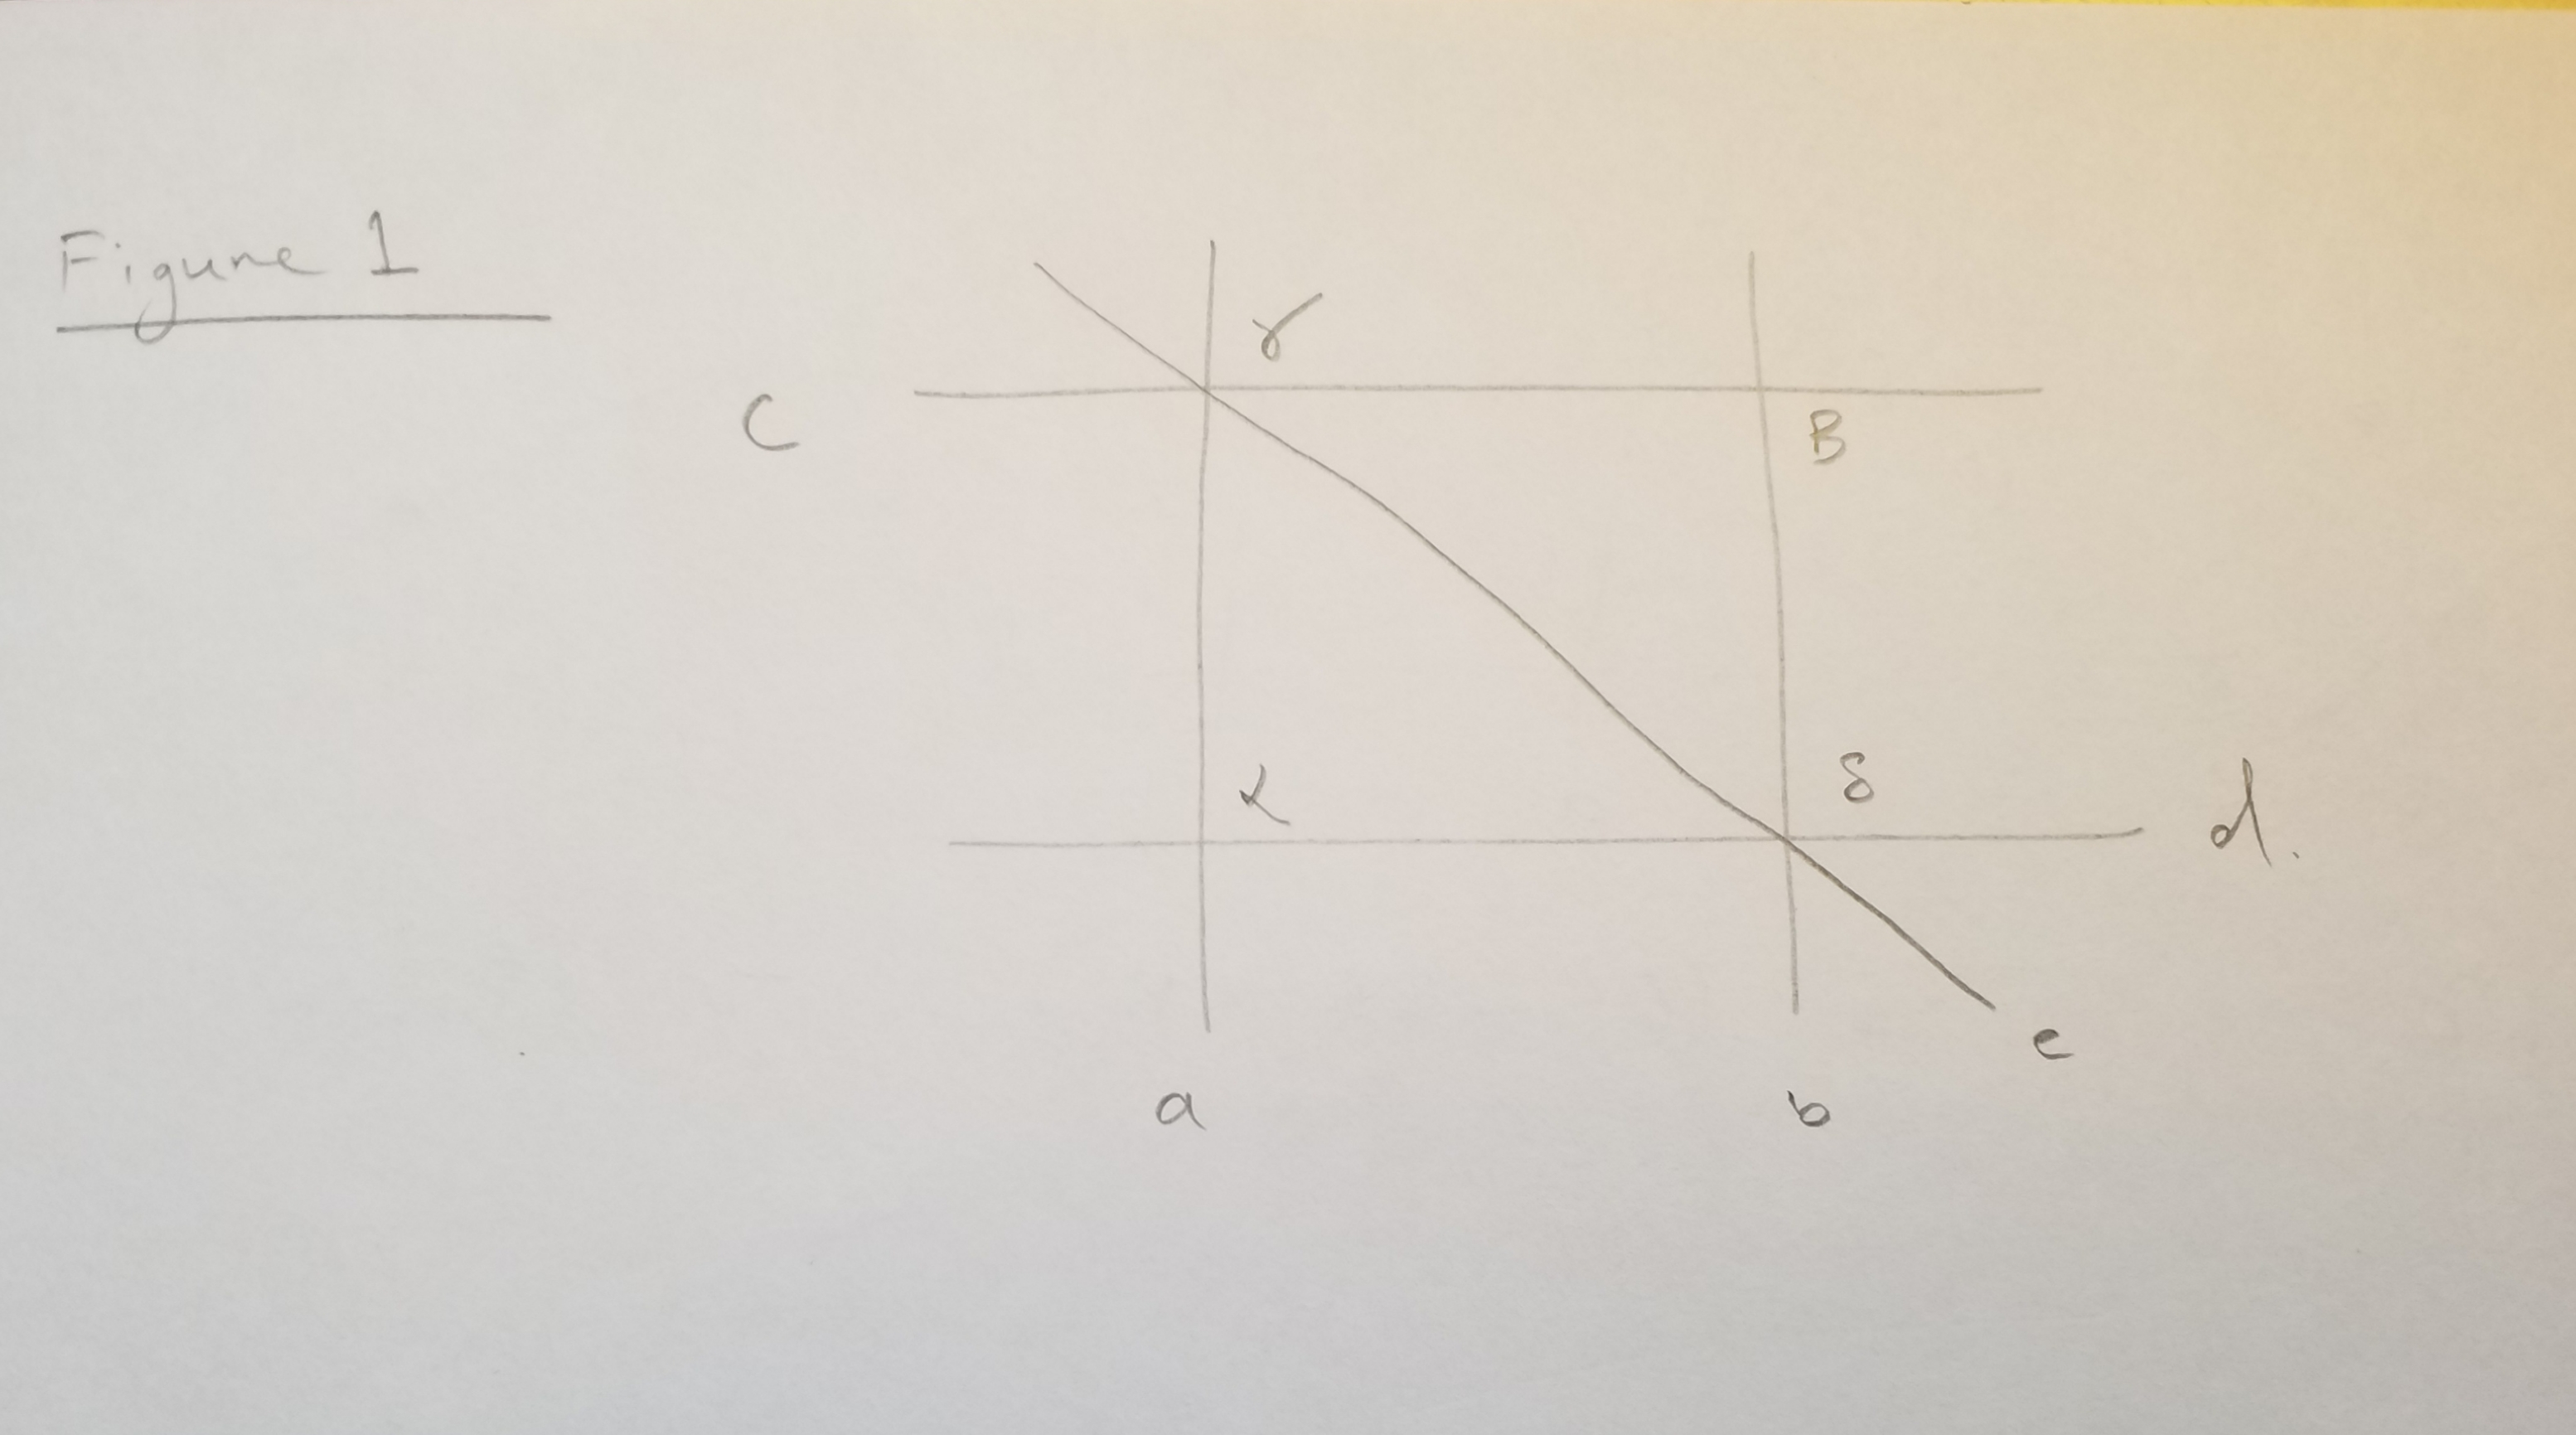
\includegraphics[scale=0.10,angle=0]{29072020 pics/fig 1.jpg}  
    \caption{Hyperplane arrangement in $\mathbb{R}^2$.}
    \label{fig 1}
\end{figure}

It is important to distinguish between unbounded and bounded regions. Note hyperplane arrangements are denoted by $\mathcal{A}$.

\begin{definition}
A region is a connected component of,
        $\mathbb{R}^n \setminus \cup_{H \in \mathcal{A}} H$. The set of regions is $\mathcal{R}(\mathcal{A})$ and the number or regions is $r(\mathcal{A})=\#\mathcal{R}(\mathcal{A})$. The term $b(\mathcal{A})$ is the number of bounded regions in the standard sense. 

\end{definition}

 \begin{definition}\label{Intposet}
 Let $\mathcal{A}$ be an arrangement in $\mathbb{R}^n$, and let $L(\mathcal{A})$ be the set of all nonempty intersections of hyperplanes in $\mathcal{A}$, including $\mathbb{R}^n$. Define $x \le y $ in $L(\mathcal{A})$ if $x \subseteq y$. That is $L(\mathcal{A})$ is partially ordered by reverse inclusion. Call $L(\mathcal{A})$ the intersection poset of $\mathcal{A}$.
 \end{definition}
 
 These intersections are often called flats. We assign a value, $\mu(x)$, to each flat in $L(\mathcal{A})$.

\begin{definition}\label{mob} Let $P$ be a locally finite poset. Define the Möbius function to be $\mu : Int(P) \rightarrow \mathbb{Z}$ by 

\begin{align*}
    \mu (x,x) &=1, \quad \forall x \in P\\
    \sum _{x \le z\le y} \mu(x,z)&=0, \quad \forall x<y \in P
\end{align*}

and $\mu(x)=\mu(\hat{0},x)$.

\end{definition}

\begin{remark}
  Each hyperplane has mobius value $-1$.
\end{remark}

\begin{example}{Example of intersection poset with mobius values and with non-generic line in $\mathbb{R}^2$}
\begin{figure}[H]
    \centering
 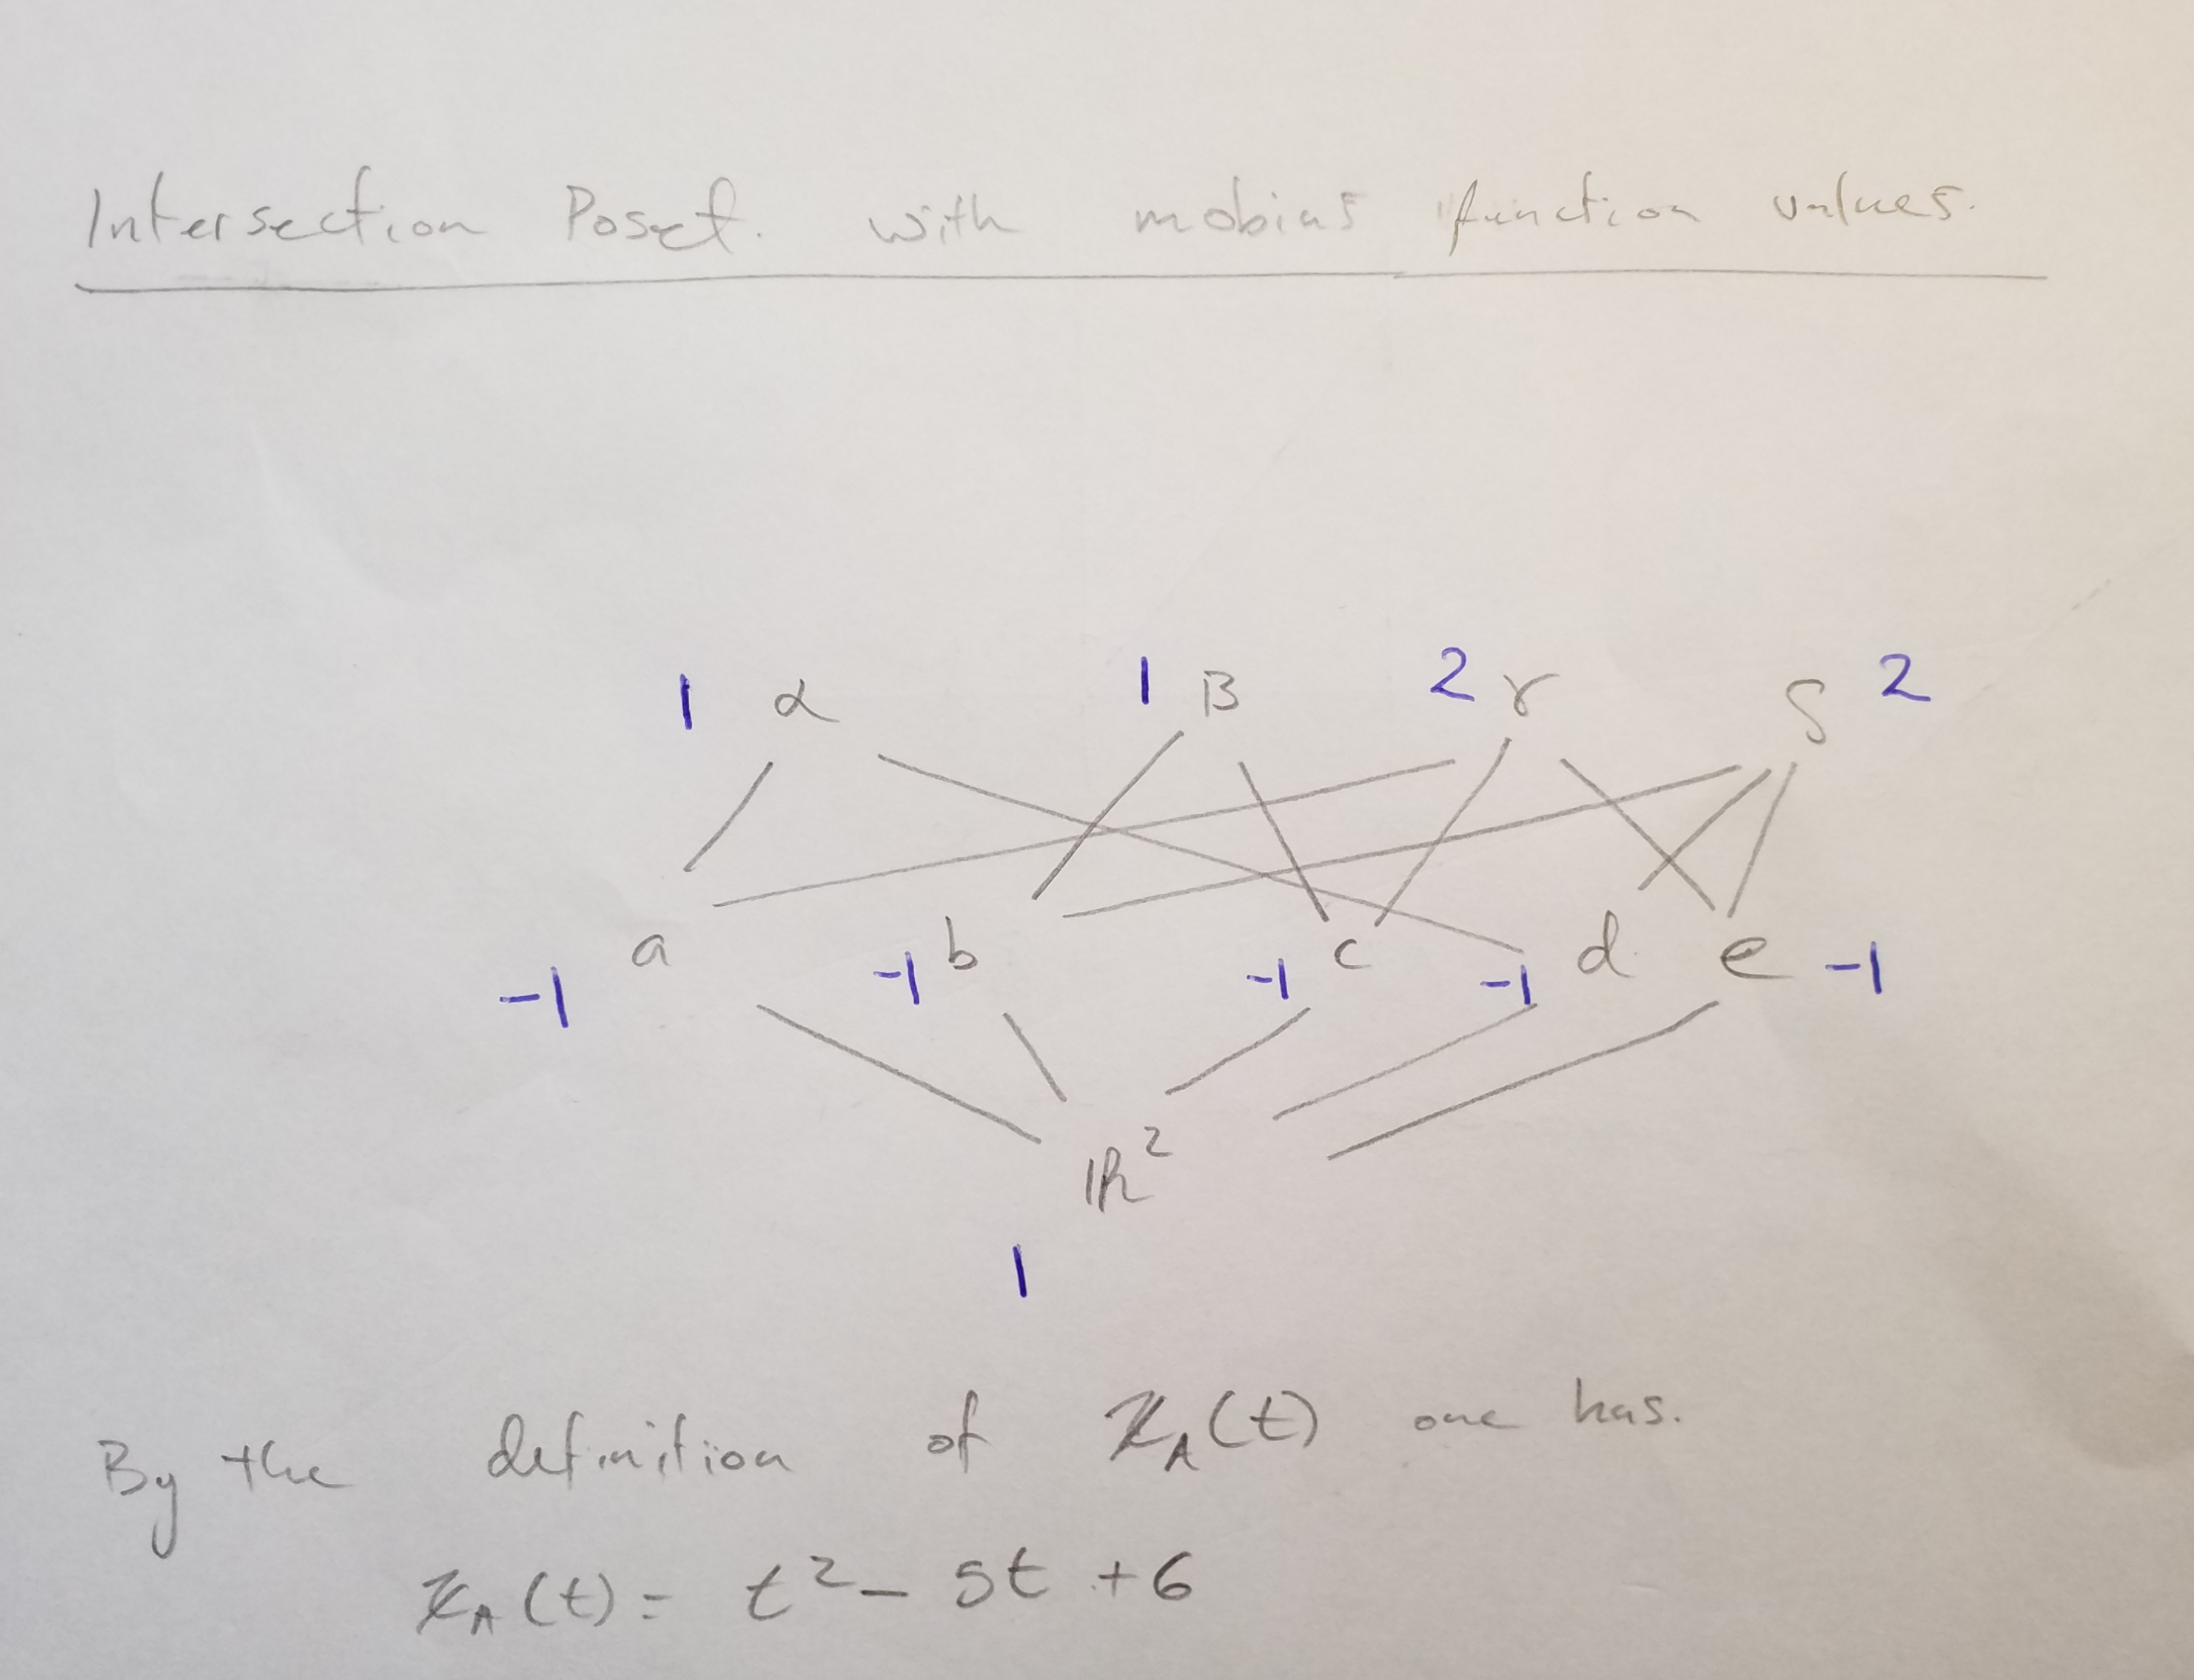
\includegraphics[scale=0.10,angle=0]{29072020 pics/poset.jpg}  
    \caption{Intersection poset of Figure 1 with Möbius values.}
    \label{poset1}
\end{figure}
\end{example}

 \begin{remark}
    In $\mathbb{R}^2$ lines are either parallel or intersect at a point, points either live outside of line or embedded in a line. In $\mathbb{R}^3$ planes either intersect giving a line or are parallel. For lines and planes, either lines are embedded, intersect at a point or are disjoint. By generic we mean, we exclude the special cases of what we mentioned above. For a total space of dimension $n$, with $k$ hyperplanes in general position, when all hyperplanes intersect they give a "subspace/set" of $codim = k$. Non-generic behaviour effects the mobius value. The flat $\gamma$ in Figure \ref{poset1} is not generic as we get a point and expect the empty set. If hyperplanes are in generic position, this gives a total of $2^k$ regions.
 \end{remark}
 

\begin{definition}
The characteristic polynomial $\chi_{{\mathcal{A}}} (t)$ of $\mathcal{A}$ is,

$$\chi_{\mathcal{A}} (t) = \sum_{x \in L(\mathcal{A})}  \mu (x) t ^{\text{dim} (x)} $$
\end{definition}

\begin{example}

This is an example of a central arrangement with which is non-generic in $\mathbb{R}^3$.

\begin{figure}[H]
    \centering
    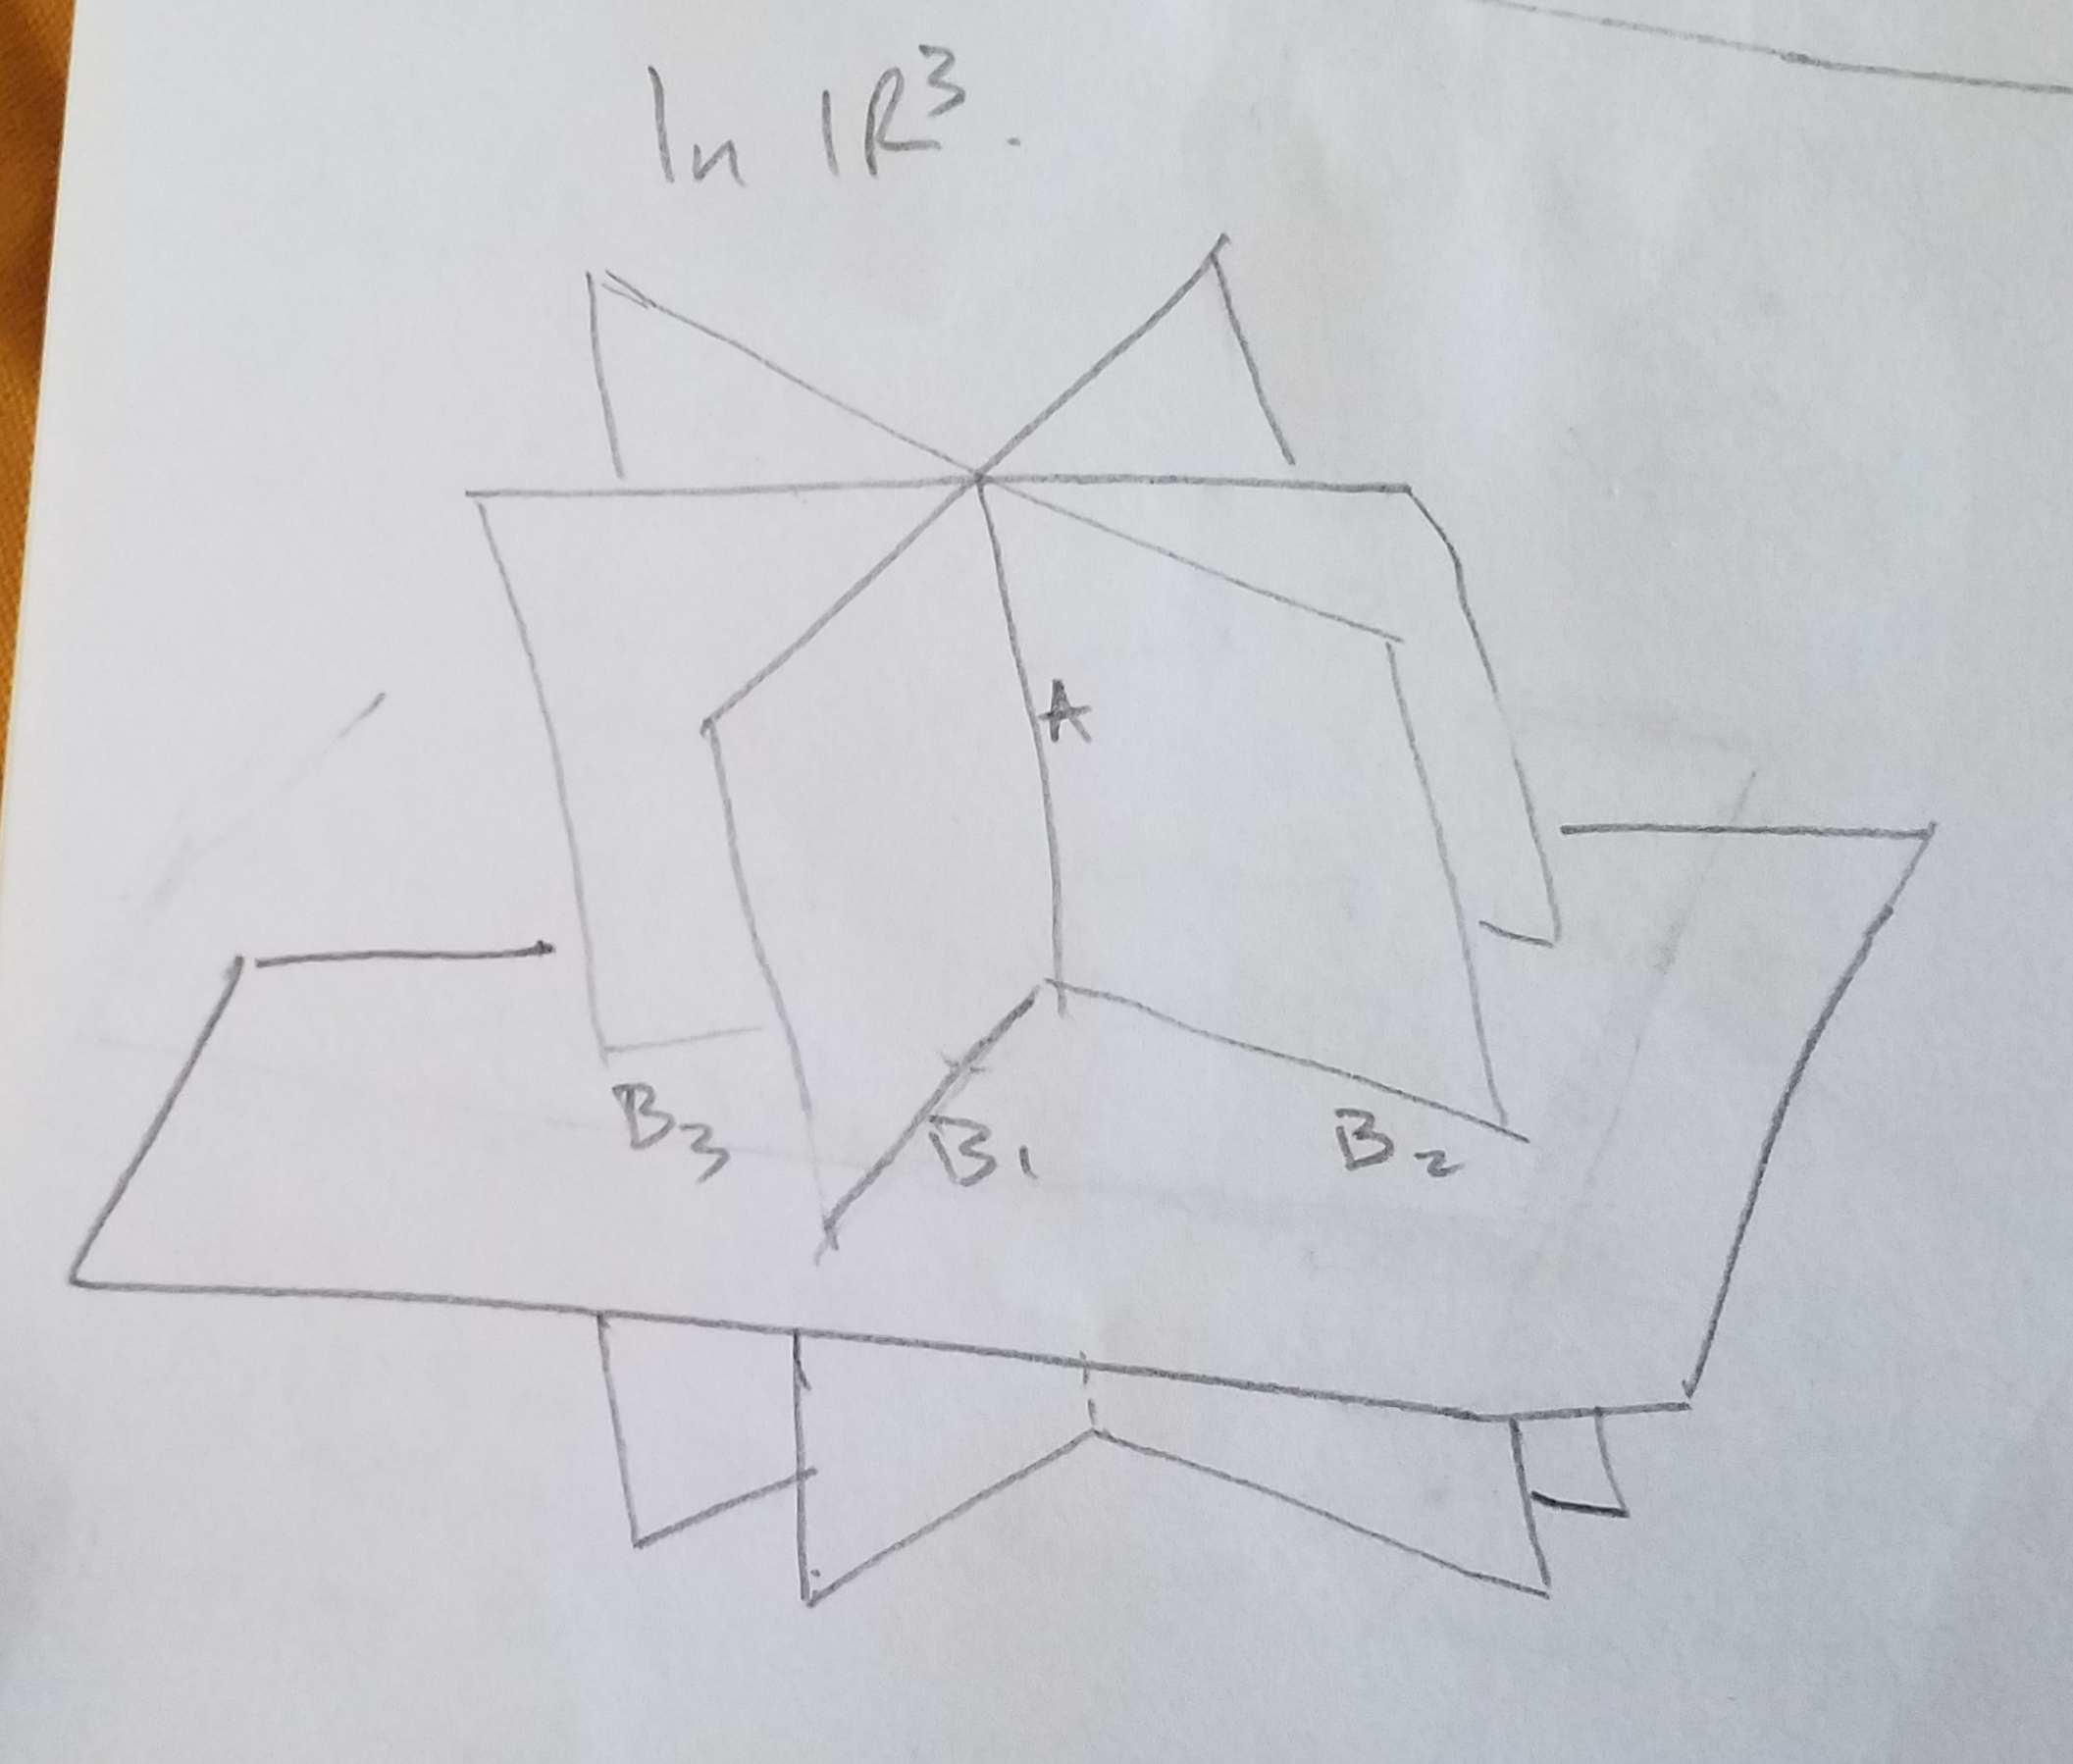
\includegraphics[width=.5\textwidth]{29072020 pics/arrg.jpg}
    \caption{Arrangement in $\mathbb{R}^3$}
    \label{Arranmgnet in R^3}
\end{figure}

Which has the following poset with associated mobius values. 

\begin{figure}[H]
    \centering
    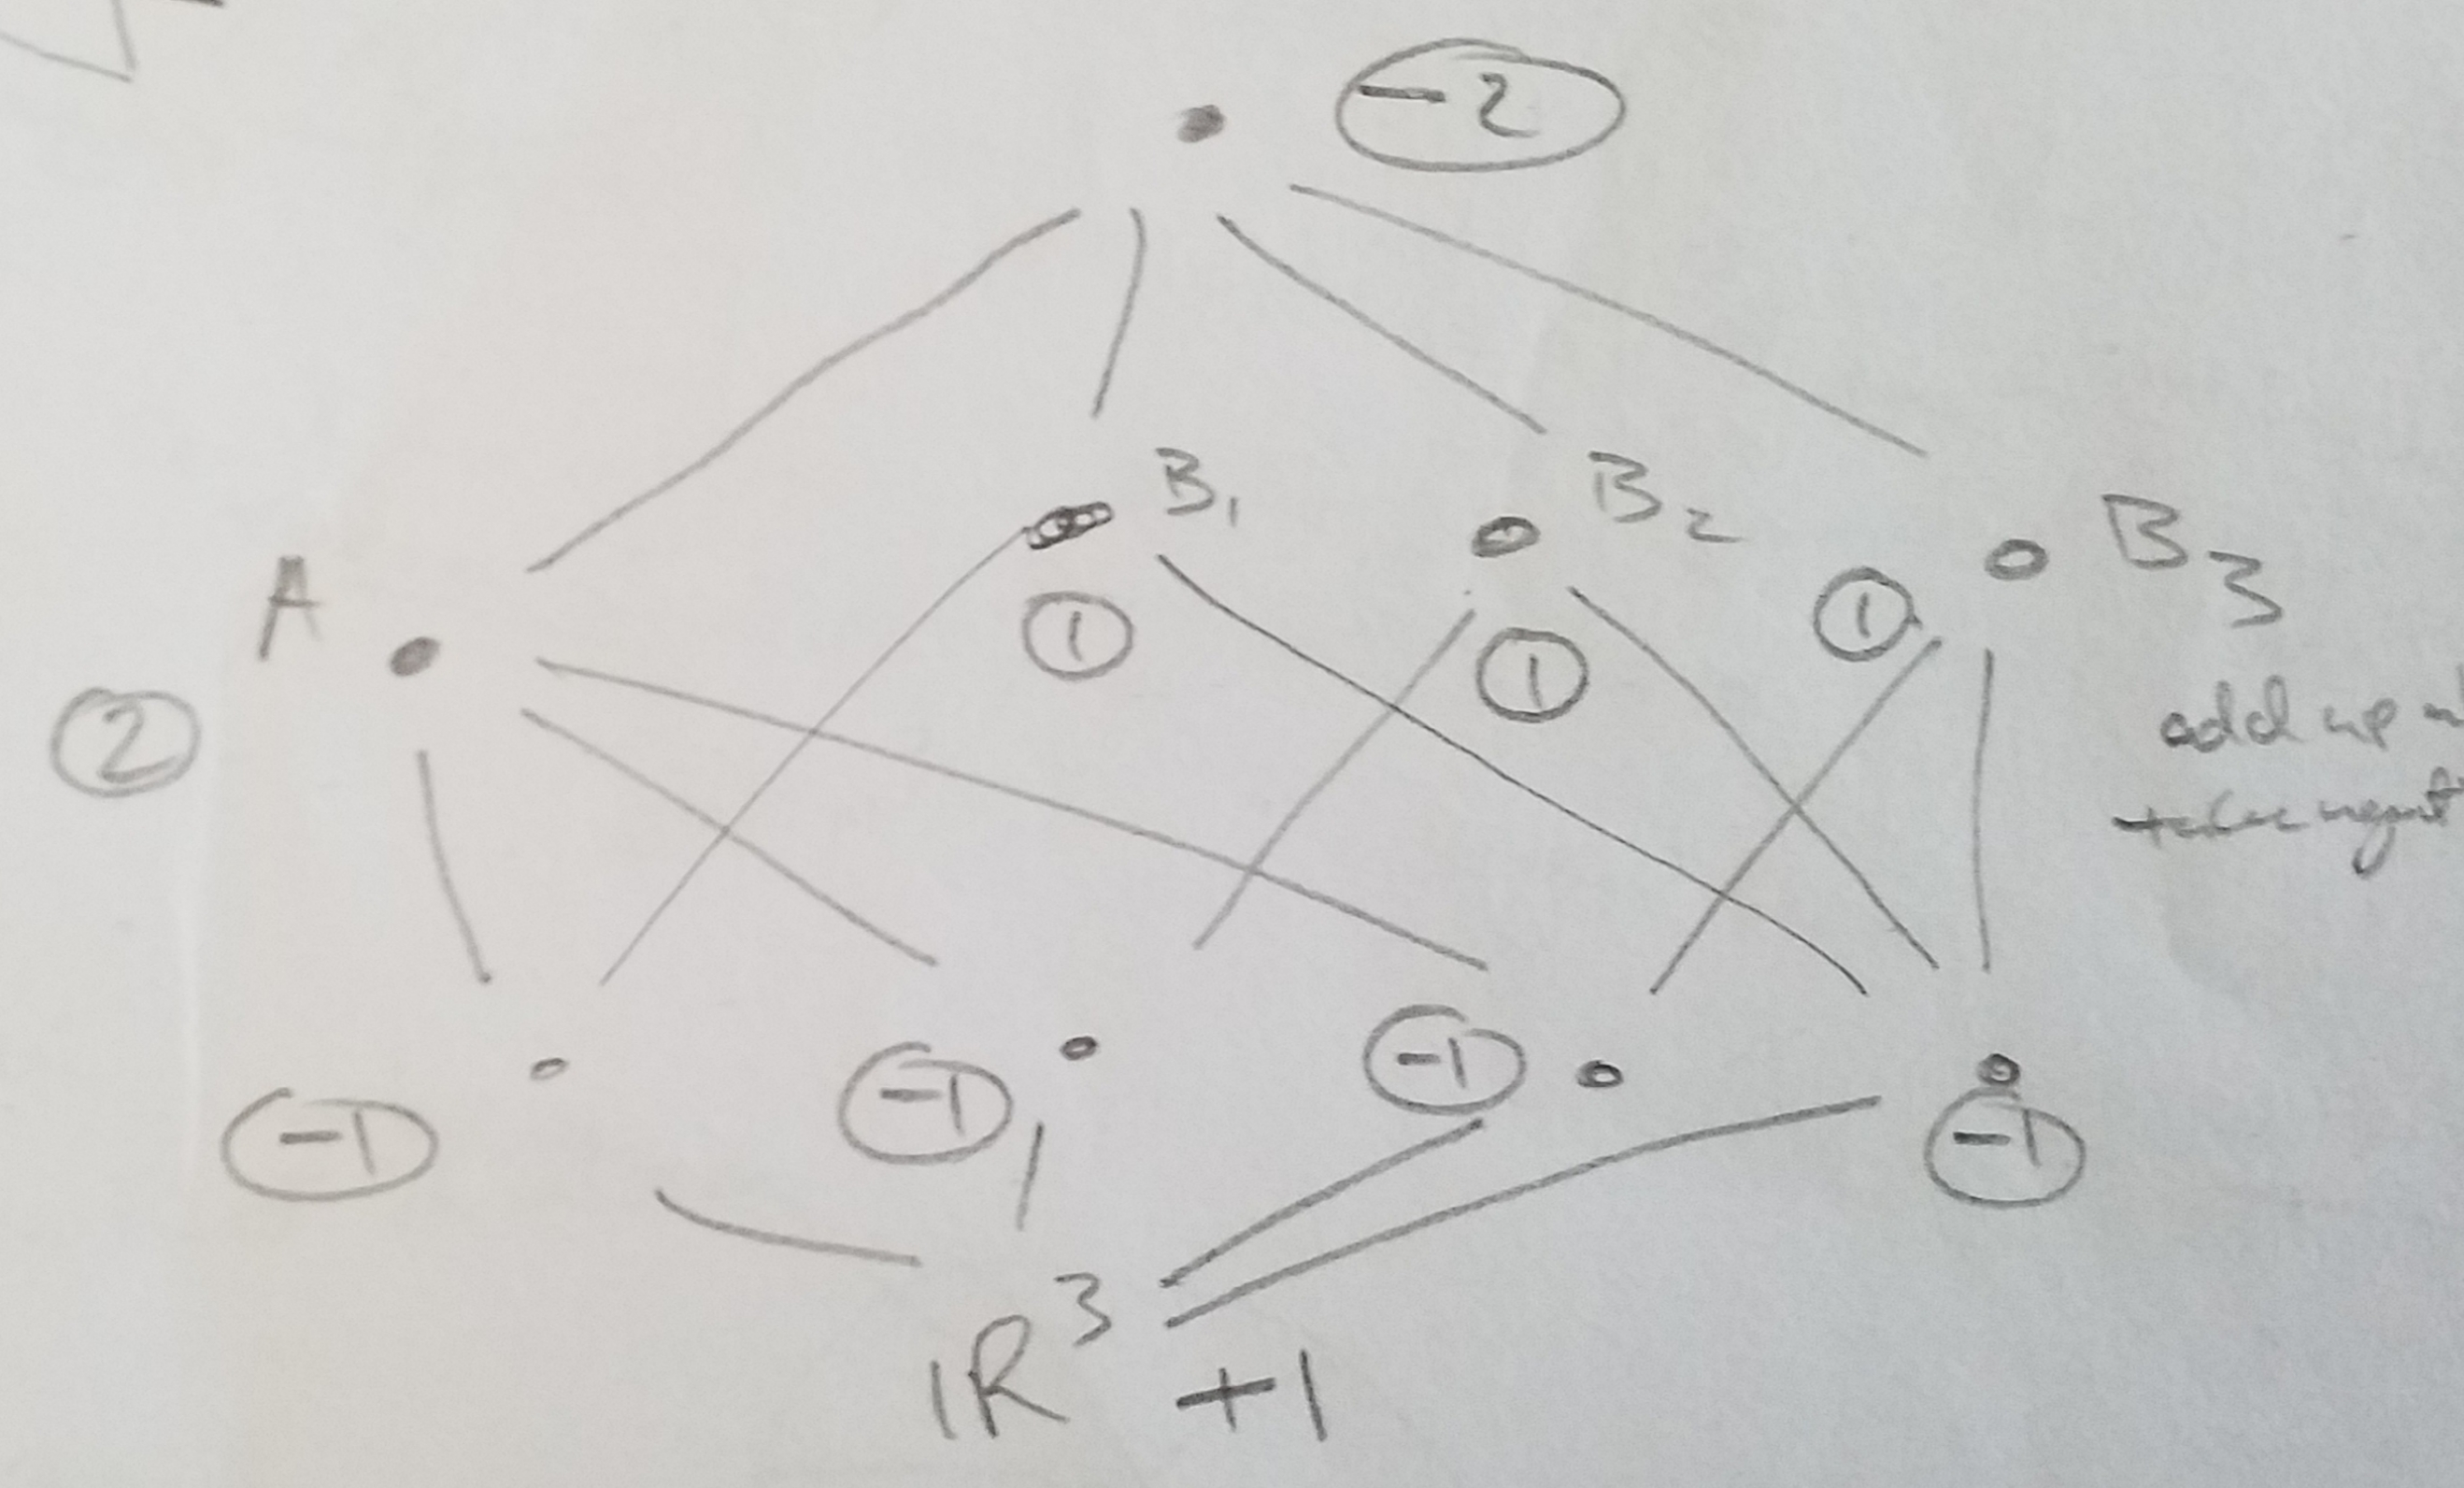
\includegraphics[width=.5\textwidth]{29072020 pics/posetarrg.jpg}
    \caption{Poset with mobius values of Figure \ref{Arranmgnet in R^3}} 
    \label{fig:my_label}
\end{figure}



The characteristic polynomial measures the complement of the arrangement. Consider the whole space ($t^3$),then remove the hyperplanes ($-4t^2$), in doing so we removed the three lines $B_1,B_2$ and $B_3$, and the line $A$ is removed a further $2$ times, so we correct by adding ($+5t$). In adding the lines back we have two additional orgins points, so we correct with $-2$. The characteristic polynomial is hence, $\chi(\mathcal{A})=t^3-4t^2+5t-2$.
\end{example}




The rank$(\mathcal{A})$ is the dimension of the space spanned by the normal's of hyperplanes in $\mathcal{A}$, when this agrees with $dim(\mathcal{A})=dim(\mathbb{R}^n$, $\mathcal{A}$ is called essential. One obtains this through the process of essentialization.  

\begin{theorem}\label{Zas}[Zaslavsky's theorem, \cite{stanley2004introduction}, Thm 2.5, p.19] Let $\mathcal{A}$ be an arrangement in $\mathbb{R}^n$. Then $r(\mathcal{A})=(-1)^n \chi_{\mathcal{A}} (-1)$ and $b(\mathcal{A})=(-1)^{\text{rank}(\mathcal{A}) }  \chi_{\mathcal{A}} (1)$. 

\end{theorem}

In order to determine $b(\mathcal{A})$ in the case of $H(S,k)$, we need to know $\chi_{{\mathcal{A}}} (t)$. The issue here, is to determine $L(\mathcal{A})$ and $\mu(x)$ for large $n$, (\cite{Etu} gives a program for this however it grows exponentially with $n$). 

\subection{Applying Zaslavsky's Theorem to the Resonance Arrangement in $\mathbb{R}^2$ and $\mathbb{R}^3$}

Consider the following arrangement, where all hyperplanes are positioned at the origin. The number of regions for each $n$, belong to the following OEIS reference: A034997.

\begin{example}
Take the $\mathbb{R}^2$ case with $x=0,y=0, x+y=0$. 

\begin{figure}[H]
    \centering
 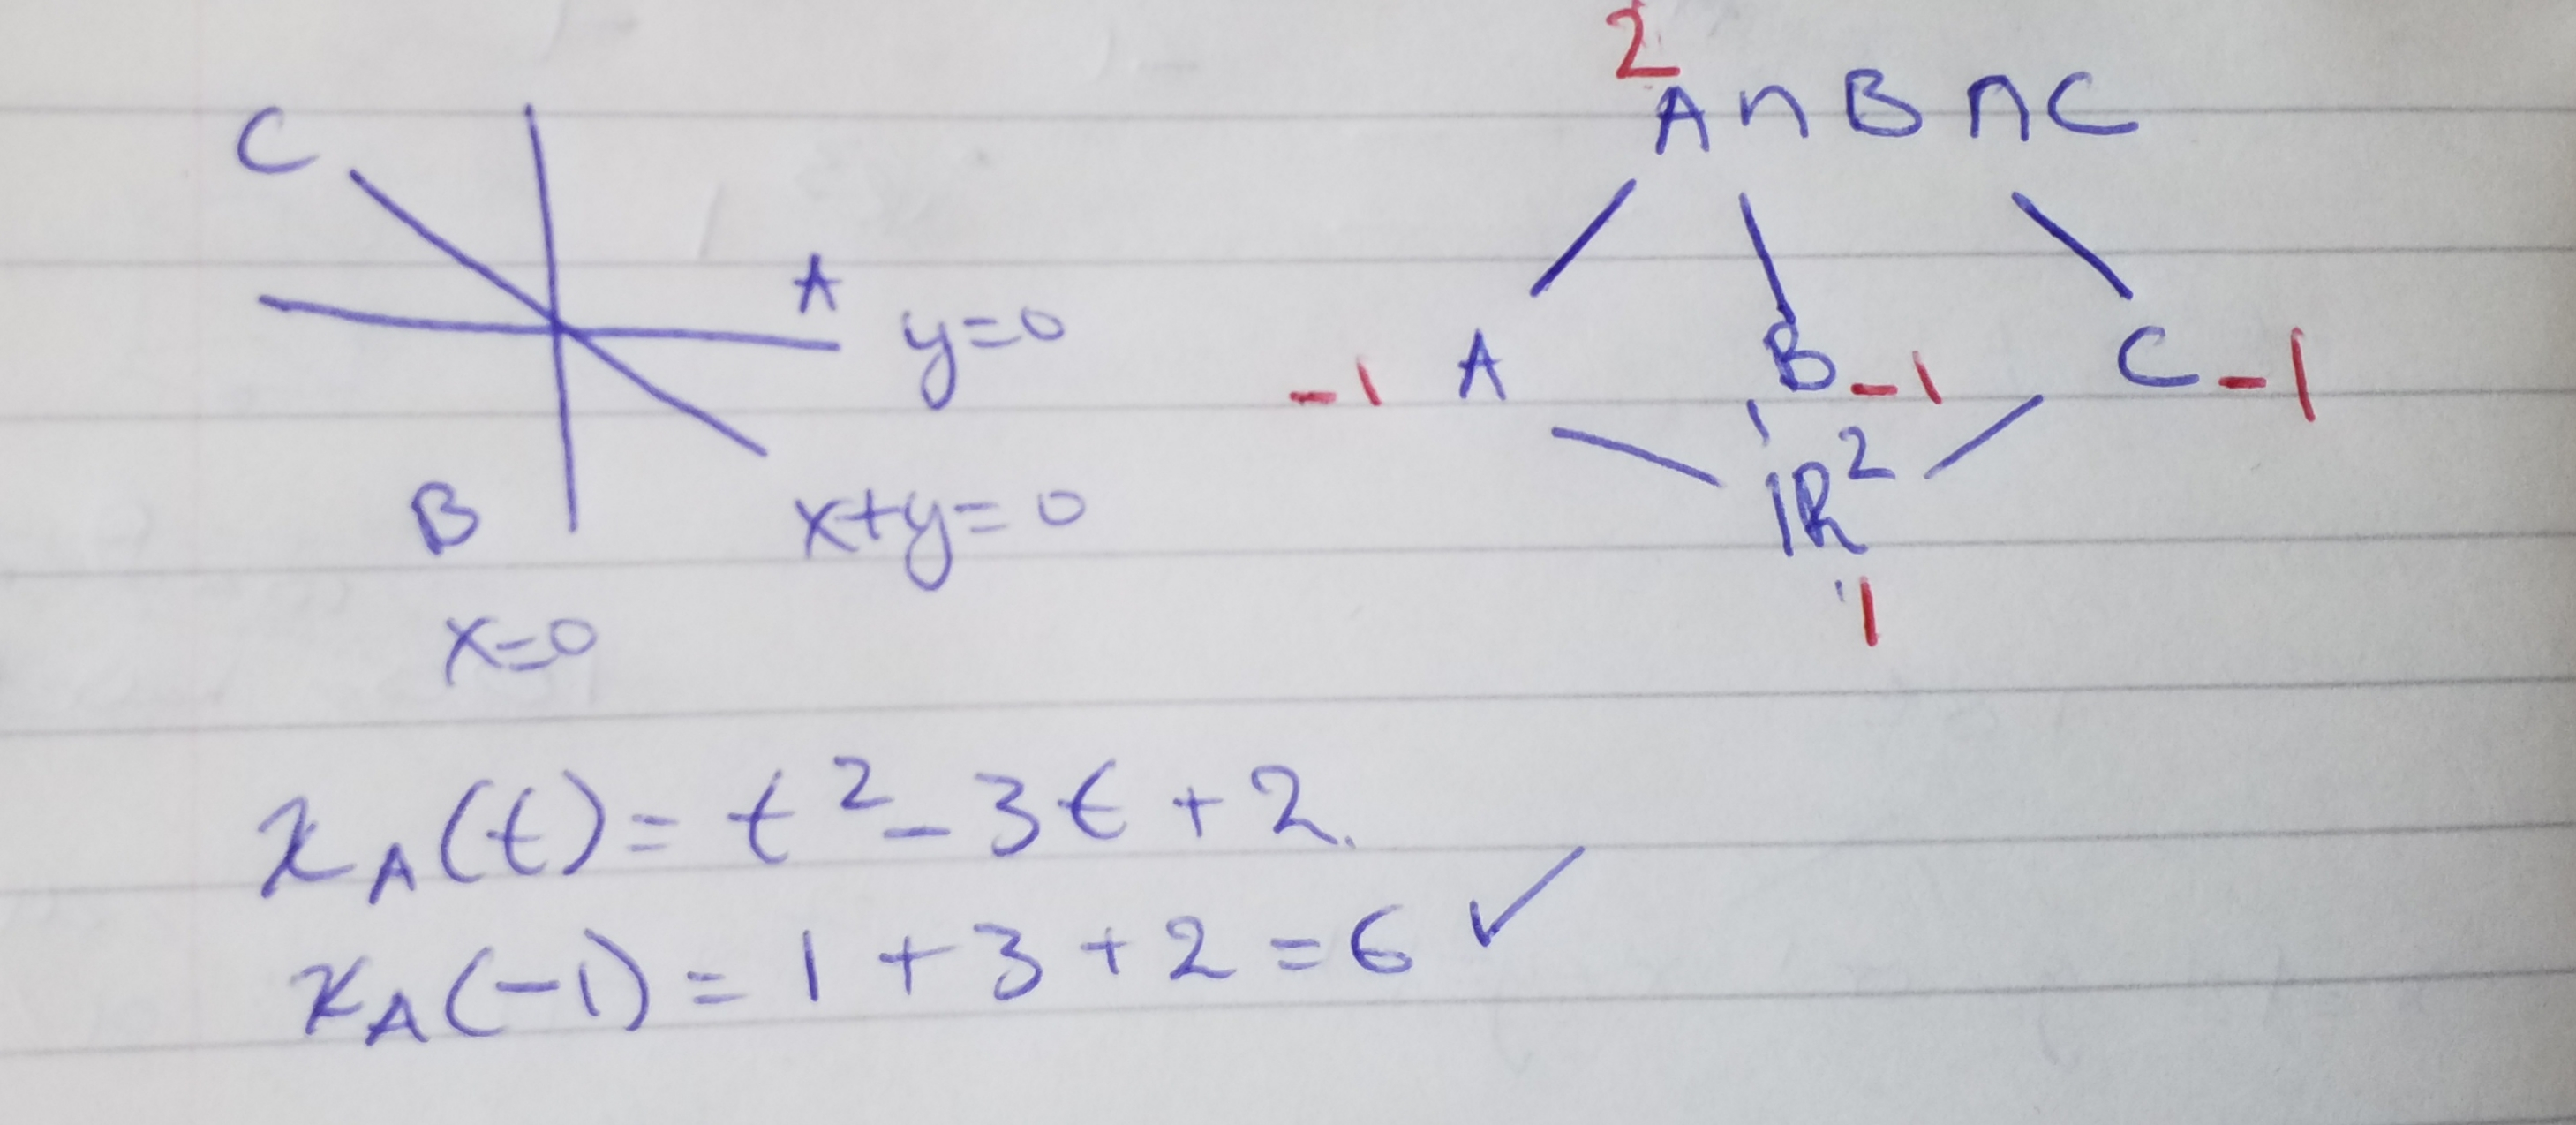
\includegraphics[scale=0.10,angle=0]{29072020 pics/resonance R2.jpg}  
    \caption{Number of region resonance arrangement $\mathbb{R}^2$}
    \label{res}
\end{figure}
\end{example}


\begin{example}
Apply Zaslavsky's theorem to the $\mathbb{R}^3$ resonance arrangement case.

\begin{figure}[H]
    \centering
 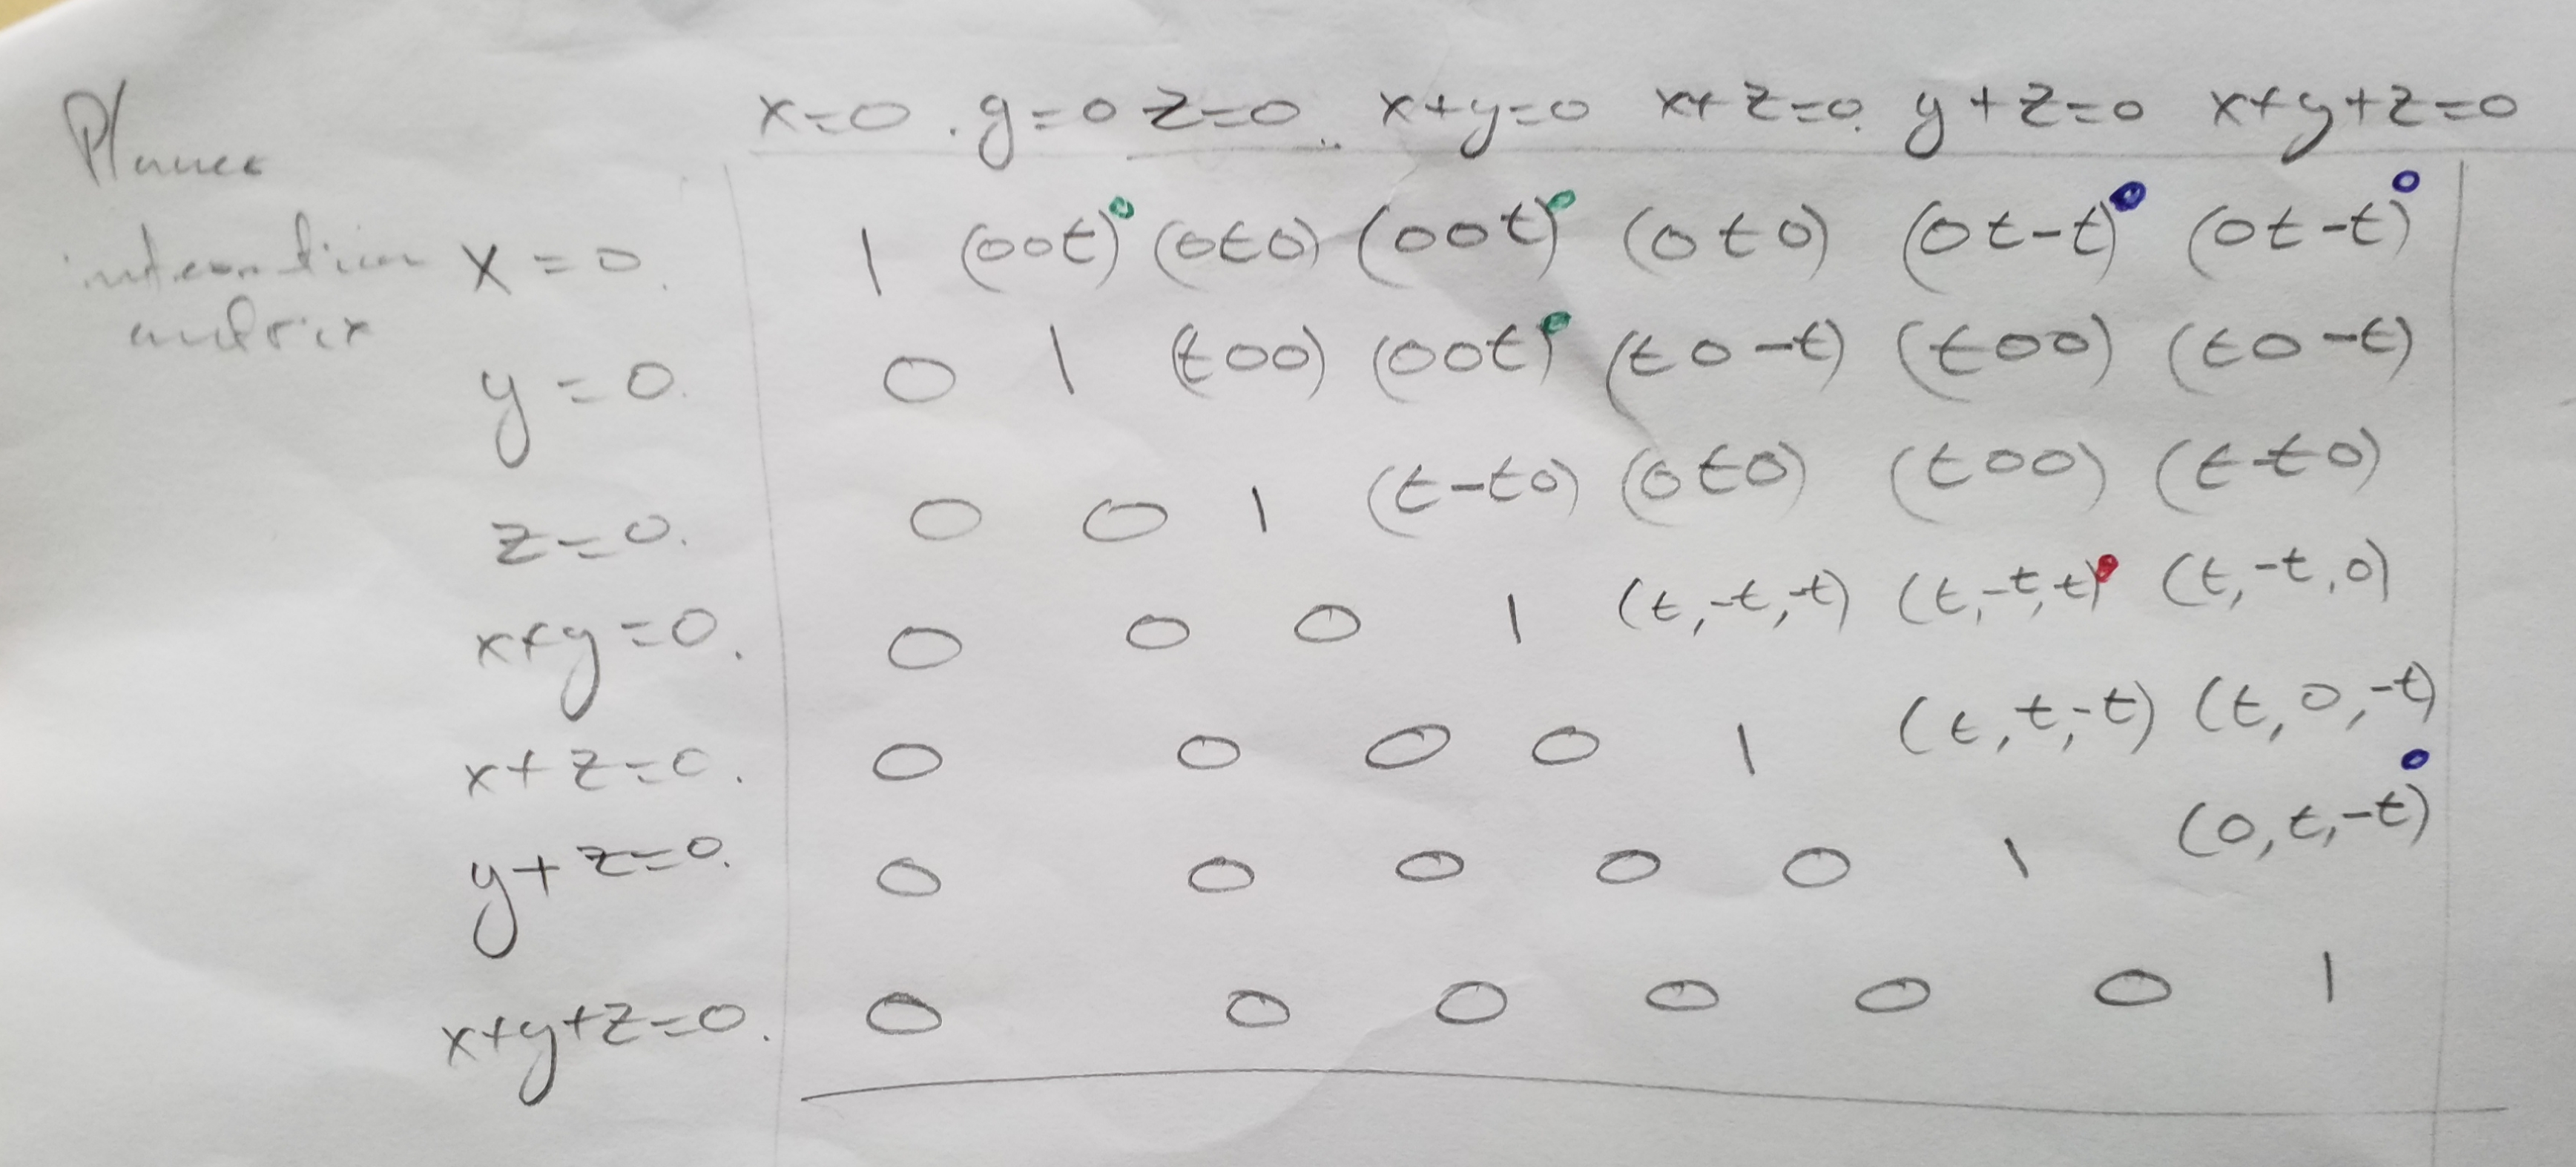
\includegraphics[scale=0.10,angle=0]{29072020 pics/resplaneeintersect.jpg}  
    \caption{Plane intersection matrix }
    \label{res}
\end{figure}



All planes intersect at the origin and recall each plane has mobius value $-1$. Each line that appears once in Figure \ref{res} is from two separate planes and so has mobius value $1$. If it appears three times it is from three planes and of mobius value $2$. We summaries this data as,

\begin{center}
\begin{tabular}{ |c|c|c|c|c|c|c|c|c|c|c| } 
 \hline
Line &(0,0,t)& (0,t,0)& (t,0,0) & (t,-t,0) & (0,t,-t) & (t,0,-t) & (t,-t,t) & (t,t,-t) & (t,-t,-t) \\ 
\hline
$\mu$ &2& 2& 2& 2& 2& 2 & 1 & 1 &1\\
\hline

 \hline
\end{tabular}
  \caption{} \label{tab:sometab}
\end{center}

There are seven planes in total and the sum of the mobius values for lines is $15$. Therefore by definition \ref{mob} we have, 

$$ 1 - 7 +15 + \mu(origin)=0$$

and so $\mu(origin)=9$. Applying Zaslavsky's theorem, we have $r(\mathcal{A})= 1+7+15+9=32$ and $b(\mathcal{A})=0$. 

\end{example}



 \subsection{Applying Zaslavsky's theorem to $H(S,k)$ in the affine case of $\mathbb{R}^2$ and $\mathbb{R}^3$}

 In order to apply the classical Zavalaskys theorem (for a finite arrangement) we need to make a choice of hyperplanes from the family $H(S,k)$ (equation \ref{HSK}). In the $\mathbb{R}^2$ the choice given in Figure \ref{fig 1} gives the correct number of bounded regions if one chooses only $x+y=1$, and not for example if we choose the lines $x+y=0, x+y=1, x+y=2$.
 
 \begin{figure}[H]
    \centering
 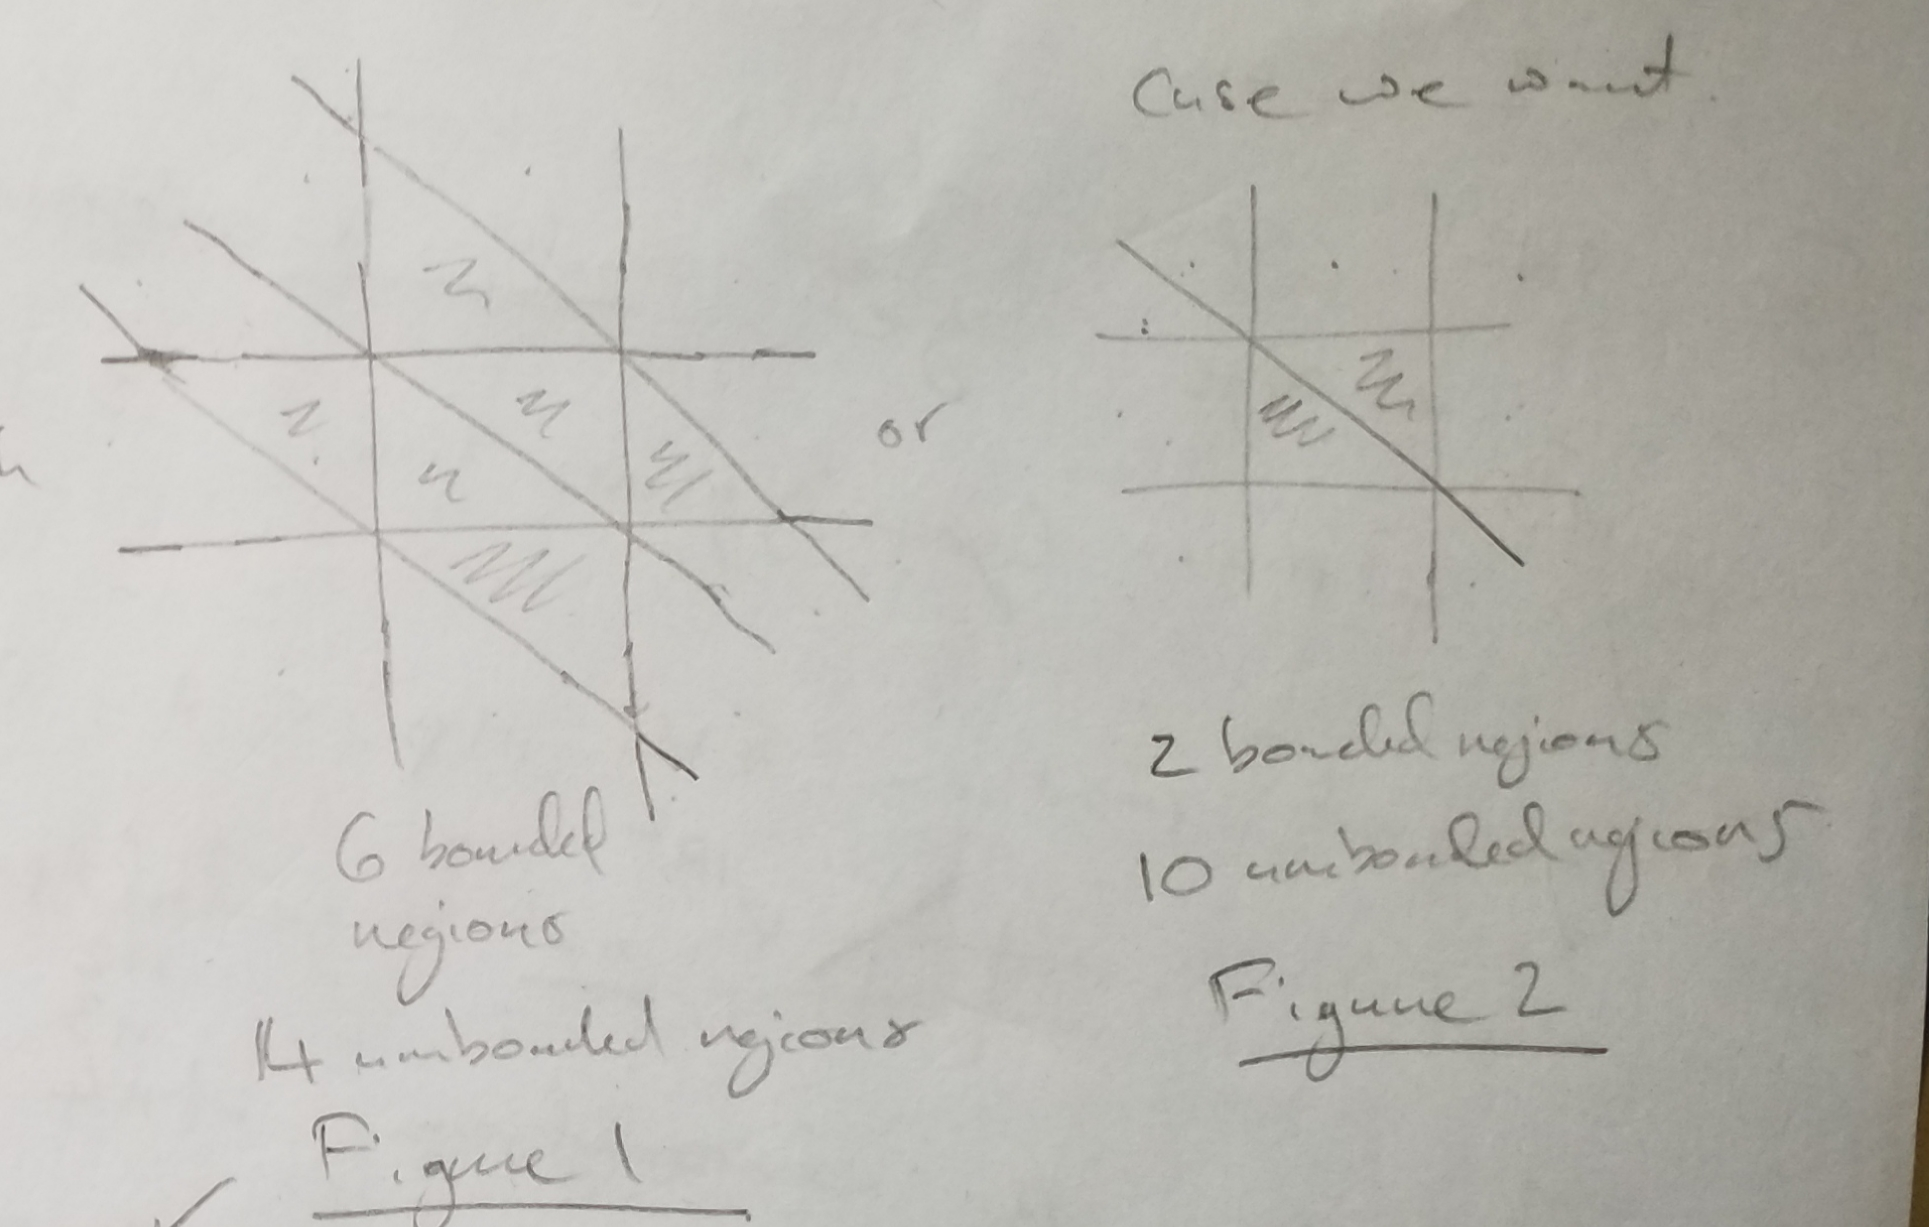
\includegraphics[scale=0.15,angle=0]{29072020 pics/n=4 choice lines.jpg}  
    \caption{Choosing the correct lines from $H(S,k)$}
    \label{fig 6}
\end{figure}
 
 Therefore we are choosing to only include those lines that intersect the interior of the square and not count those that meet the interior and boundary (left diagram of Figure \ref{fig 6}). Generalising to $\mathbb{R}^3$ case, we have the following problem. 
 
 \medskip
 To apply Zaslavsky's theorem to the following arrangement $\mathcal{A}$ given by the equations of (\ref{HSK}) and determine $b(\mathcal{A})$. We have determined (using geoalgebra and inspection) the number of bounded regions inside the cube to be $10$. Is $b(\mathcal{A}) =10$ if one constructs $L(\mathcal{A})$ and applys Zaslavsky's theorem? If we find a number greater than $10$ then the method of taking the interior planes does not work and we must find a different approach. The suggested next step is to consider toric hyperplane arrangements. 
 
\begin{example}
Consider the arrangement $\mathcal{A}$ in $\mathbb{R}^3$ of hyperplanes: $x,y,z= 0,1$, $x+y=1$, $y+z=1$, $x+z=1$, $x+y+z=1$, $x+y+z=2$. We aim to determine the intersection poset and the Möbius values of each element, then determine the characteristic polynomial, and then $b(\mathcal{A})$. First we determine the lines of intersection of all pairs of planes.

\begin{figure}[H]
    \centering
 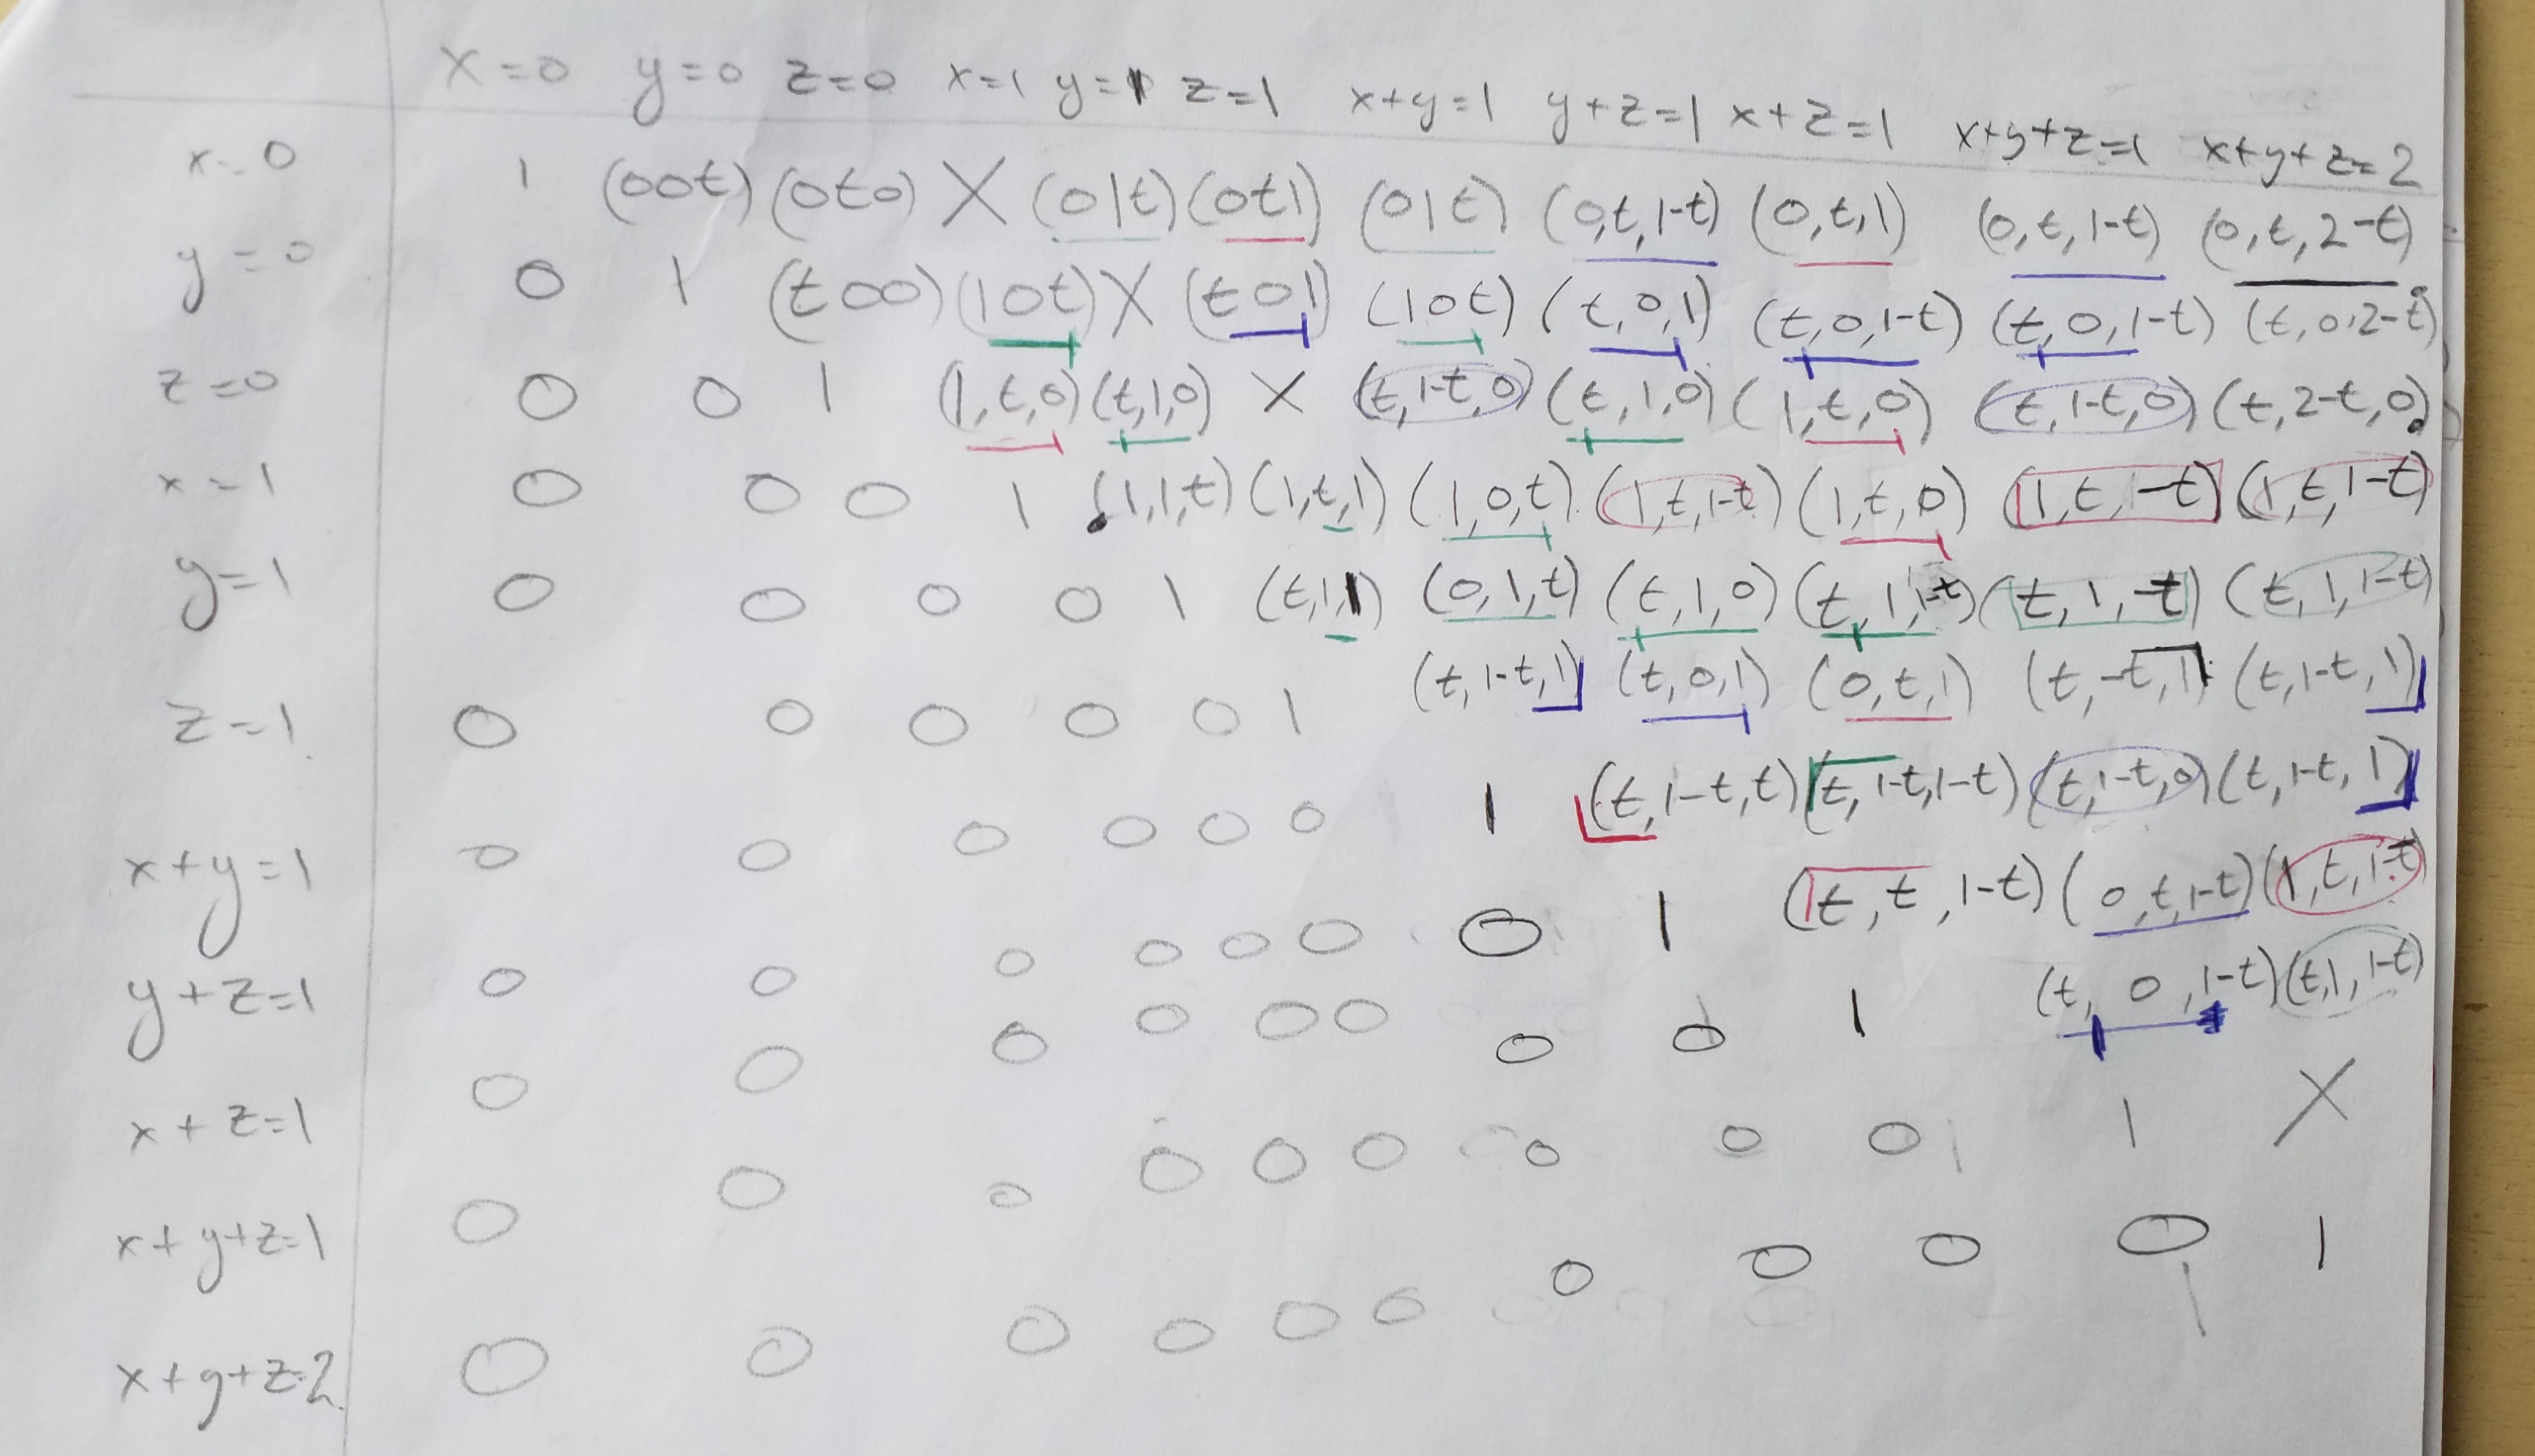
\includegraphics[scale=0.10,angle=0]{29072020 pics/planesn4g1.jpg}  
    \caption{Pairwise intersection of planes of $\mathcal{A}$}
    \label{fig 2}
\end{figure}

The following table gives each line and the number of times each appears in Figure \ref{fig 2}.

\begin{center}
\begin{tabular}{ |c|c|c|c|c|c|c|c|c|c| } 
 \hline
(0,0,t)& (0,t,0)& (t,0,0) &(0,1,t) & (0,t,1) & (1,0,t) & (t,0,1) & (1,t,0) & (t,1,0)&  (0,t,1-t)   \\ 
\hline
1&1&1&3&3&3&3&3&3&3\\
\hline
(0,t,2-t) &(t,0,1-t) &(t,0,2-t) &(t, 2-t, 0)& (t,1,1) & (1,1,t)& (1,t,1)&  (1,t,1-t)&  (1,t,-t)& (t,1,1-t)\\
\hline
1&3&1&1&1&1&1&3&1&3\\ 
\hline
(t,1,-t) &(t, -t, 1)& (t,1-t,t) &(t,t,1-t) &(t,1-t,1-t) &(t,1-t,0)  &(t,1-t,1)& & &\\
\hline
  1&1&1&1&1&3&3 & & & \\
 \hline
\end{tabular}
  \caption{} \label{tab:sometab}
\end{center}

If a line $L$ appears only one time in Figure \ref{fig 2} then it comes from two planes $P_1,P_2$ and so has Möbius value $1$ as planes have $\mu(P_i)=-1$, i.e.

$$\mu(\mathbb{R}^3) + \mu(P_1) + \mu(P_2) + \mu(L)= 1 -1 -1 + \mu(L) = 0.$$

If the line $L$ has appears $3$ times then it comes from three planes $P_1,P_2$ and $P_3$ so has Möbius value $2$. For example take $(1,0,t)$ this has planes $x=1$, $y=0$, $x+y=1$ see Figure \ref{fig 2}. For ease the following table shows lines from plane intersections and their corresponding Möbius values.

\begin{center}
\begin{tabular}{ |c|c|c|c|c|c|c|c|c|c| } 
 \hline
(0,0,t)& (0,t,0)& (t,0,0) &(0,1,t) & (0,t,1) & (1,0,t) & (t,0,1) & (1,t,0) & (t,1,0)&  (0,t,1-t)   \\ 
\hline
1&1&1&2&2&2&2&2&2&2\\
\hline
(0,t,2-t) &(t,0,1-t) &(t,0,2-t) &(t, 2-t, 0)& (t,1,1) & (1,1,t)& (1,t,1)&  (1,t,1-t)&  (1,t,-t)& (t,1,1-t)\\
\hline
1&2&1&1&1&1&1&2&1&2\\ 
\hline
(t,1,-t) &(t, -t, 1)& (t,1-t,t) &(t,t,1-t) &(t,1-t,1-t) &(t,1-t,0)  &(t,1-t,1)& & &\\
\hline
  1&1&1&1&1&2&2 & & & \\
 \hline
\end{tabular}
  \caption{} \label{tab:sometab}
\end{center}



So far we have examined the intersection of two planes. Following definition \ref{Intposet} we now consider the generic intersection of three planes, which is the same as the intersection of a line and a plane which intersects generically at a point. Figure \ref{fig 3} shows the intersection of all lines obtained from the intersection of two planes with all planes involved. Where $L$ denotes the line is embedded in the plane, $X$ denotes the line disjoint from the plane. 

\begin{figure}[H]
    \centering
 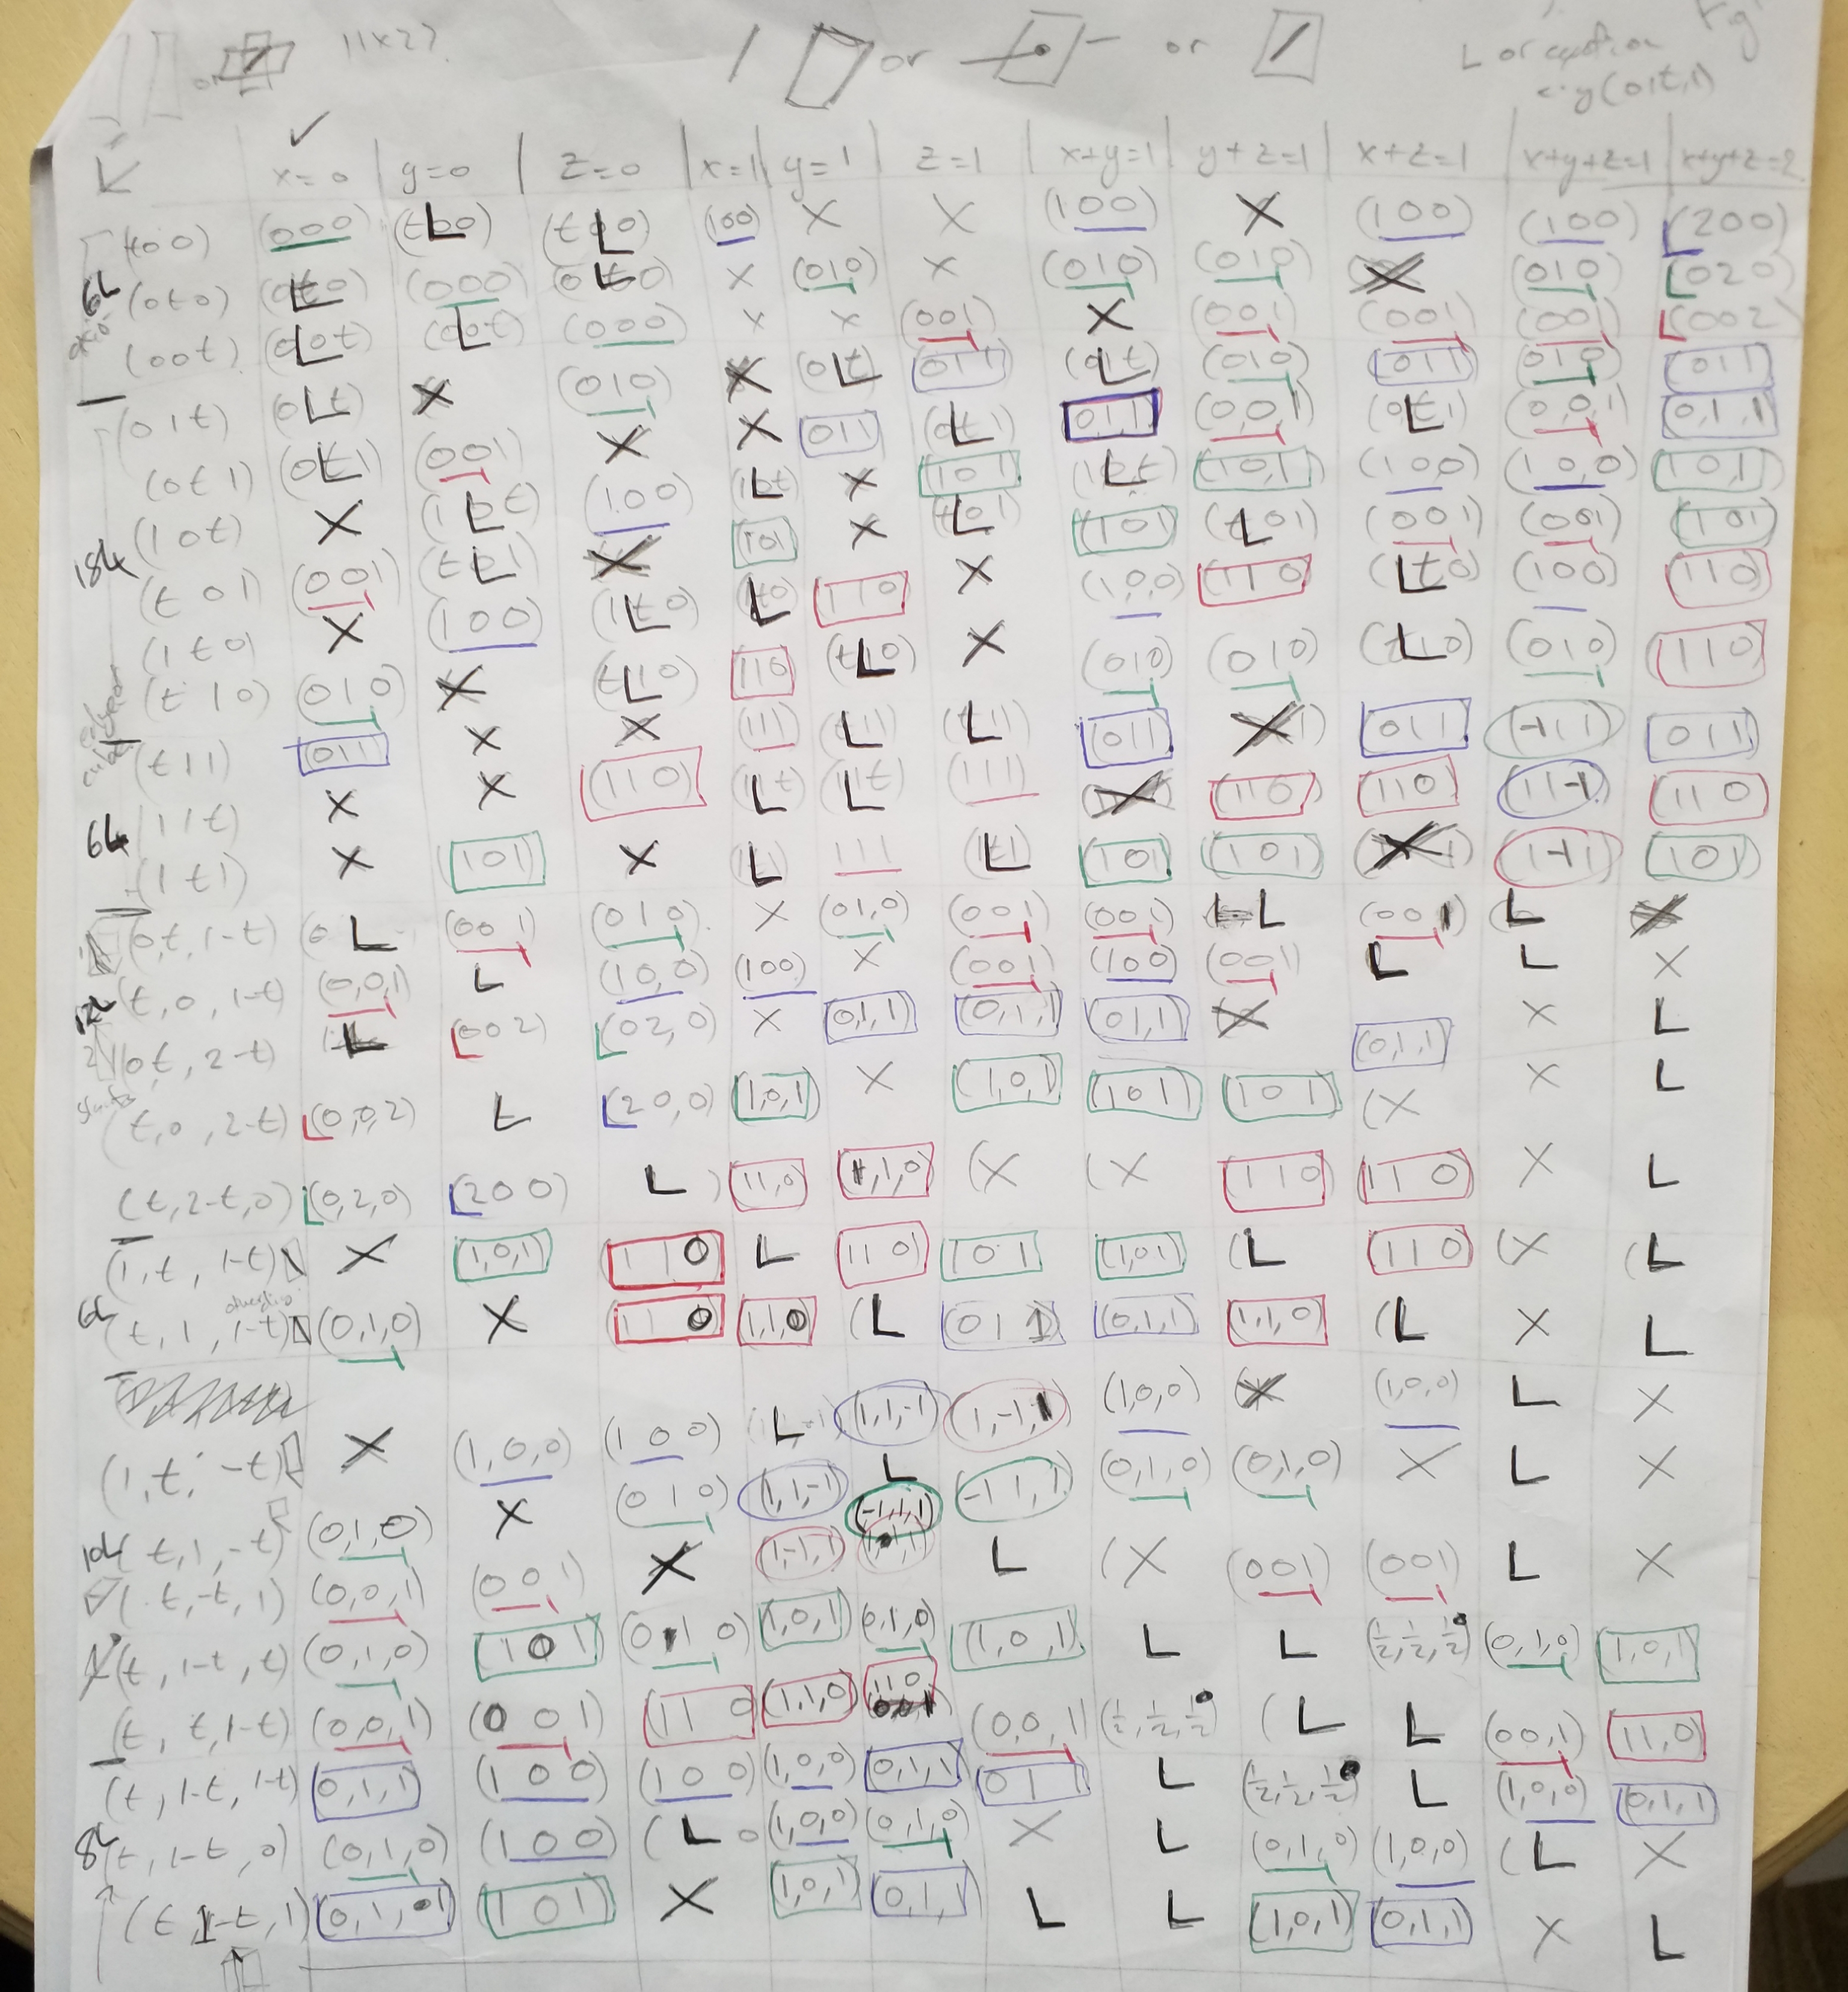
\includegraphics[scale=0.10,angle=0]{29072020 pics/lineplaneint.jpg}  
    \caption{Intersection of lines and planes}
    \label{fig 3}
\end{figure}

We are only interested in the points as the $\mu$ values for lines have already been determined. 

%The number of $L$ are 66.

\begin{remark} Note the points $(2,0,0), (0,2,0), (0,0,2), (-1,1,1),(1,-1,1) ,(1,1,-1)$, these give $6$ bounded tetrahedron regions on the faces of the cube.Once we show the number of bounded region inside the cube is $10$, then we will have $b(\mathcal{A}) \ge 16$, contradicting what we wanted at the start.
\end{remark}


Next we determine the mobius values for the points. For this we need to know which plane each point belongs to and the number of planes. 

\begin{figure}[H]
    \centering
 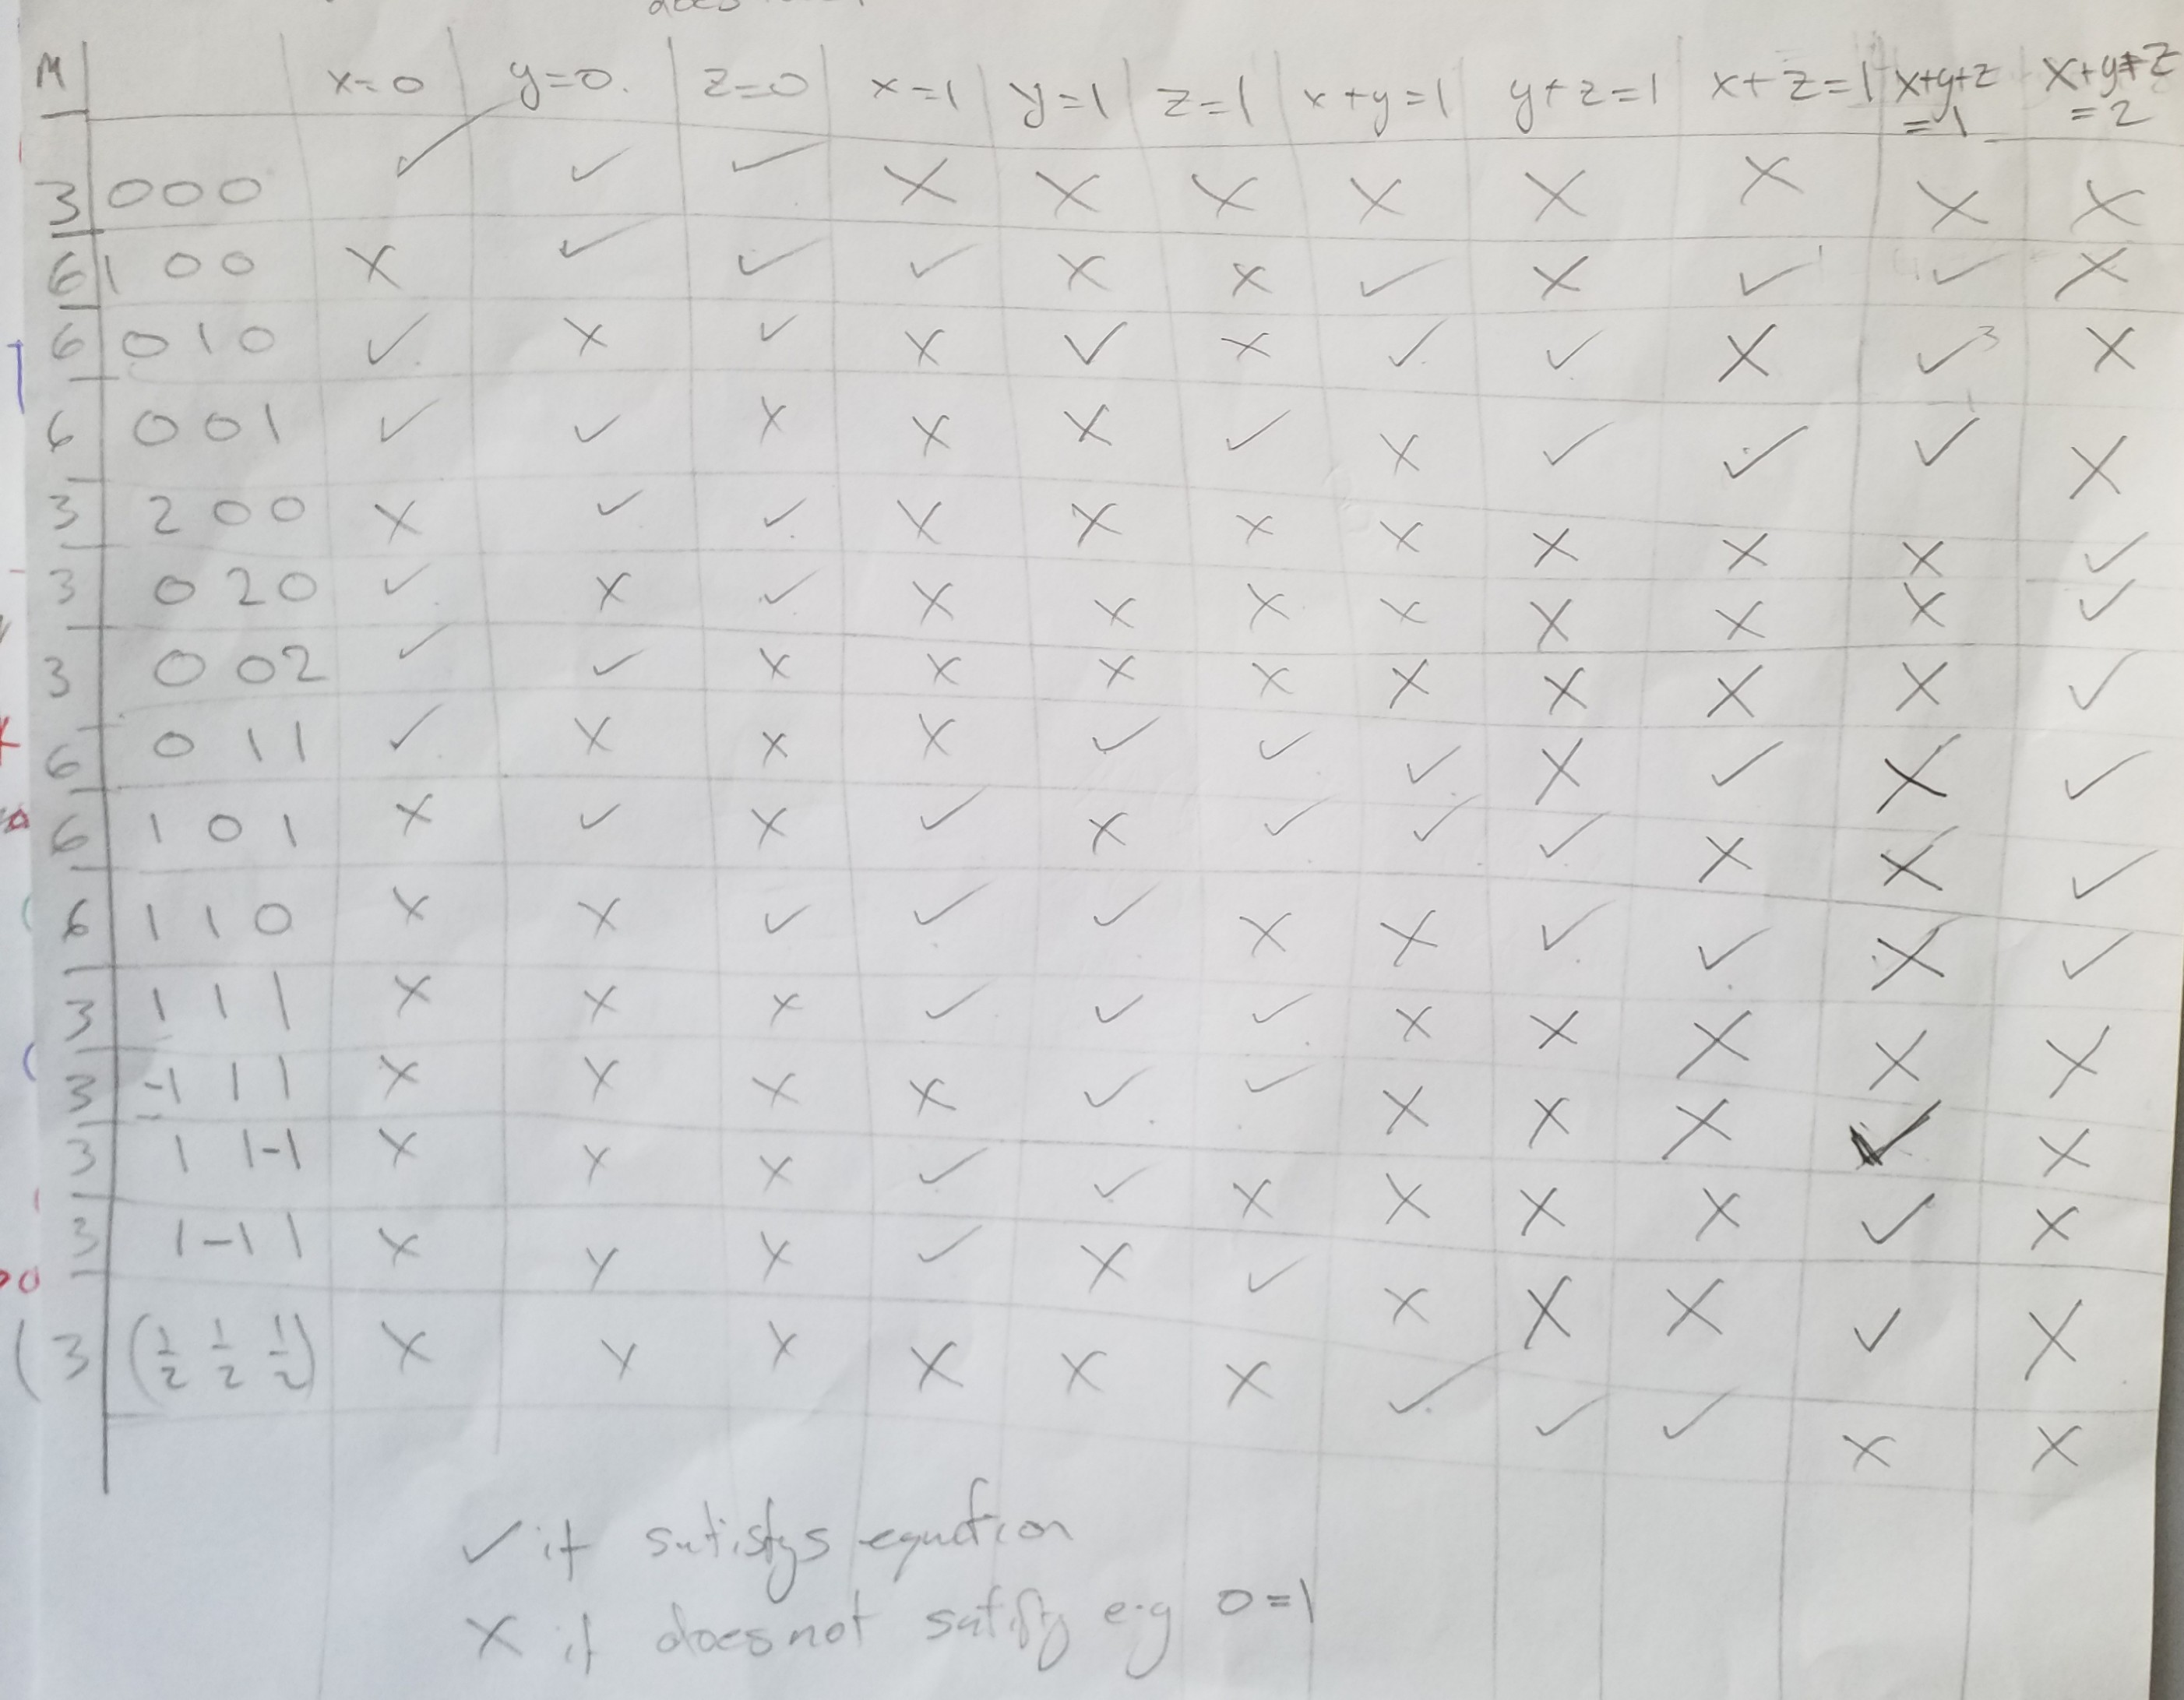
\includegraphics[scale=0.10,angle=0]{29072020 pics/Pointsplane.jpg}  
    \caption{Points in planes}
    \label{pointsplanes}
\end{figure}


 From Figure \ref{fig 3} we can find which planes have the given coordinate. For example the point $(1,1,0)$ is given by $z=0, x=1, y=1, x+y=1,y+z=1, x+z=1, x+y+z=1$ which can be seen in Geoalgebra. We also know from Figure \ref{fig 3} which lines have each point lying in them. From this we can get the Möbius value for the point by noting the number of planes and the sum of mobius values for the lines containing each point. 
 
\medskip

As all planes have the same Möbius value $-1$. We therefore only need to count the number of planes that give the point (the number of times it appears in different columns in Figure \ref{fig 3}). Note the $\mu$ value for the lines differ so we need to keep track of them. 

\begin{figure}[H]
    \centering
 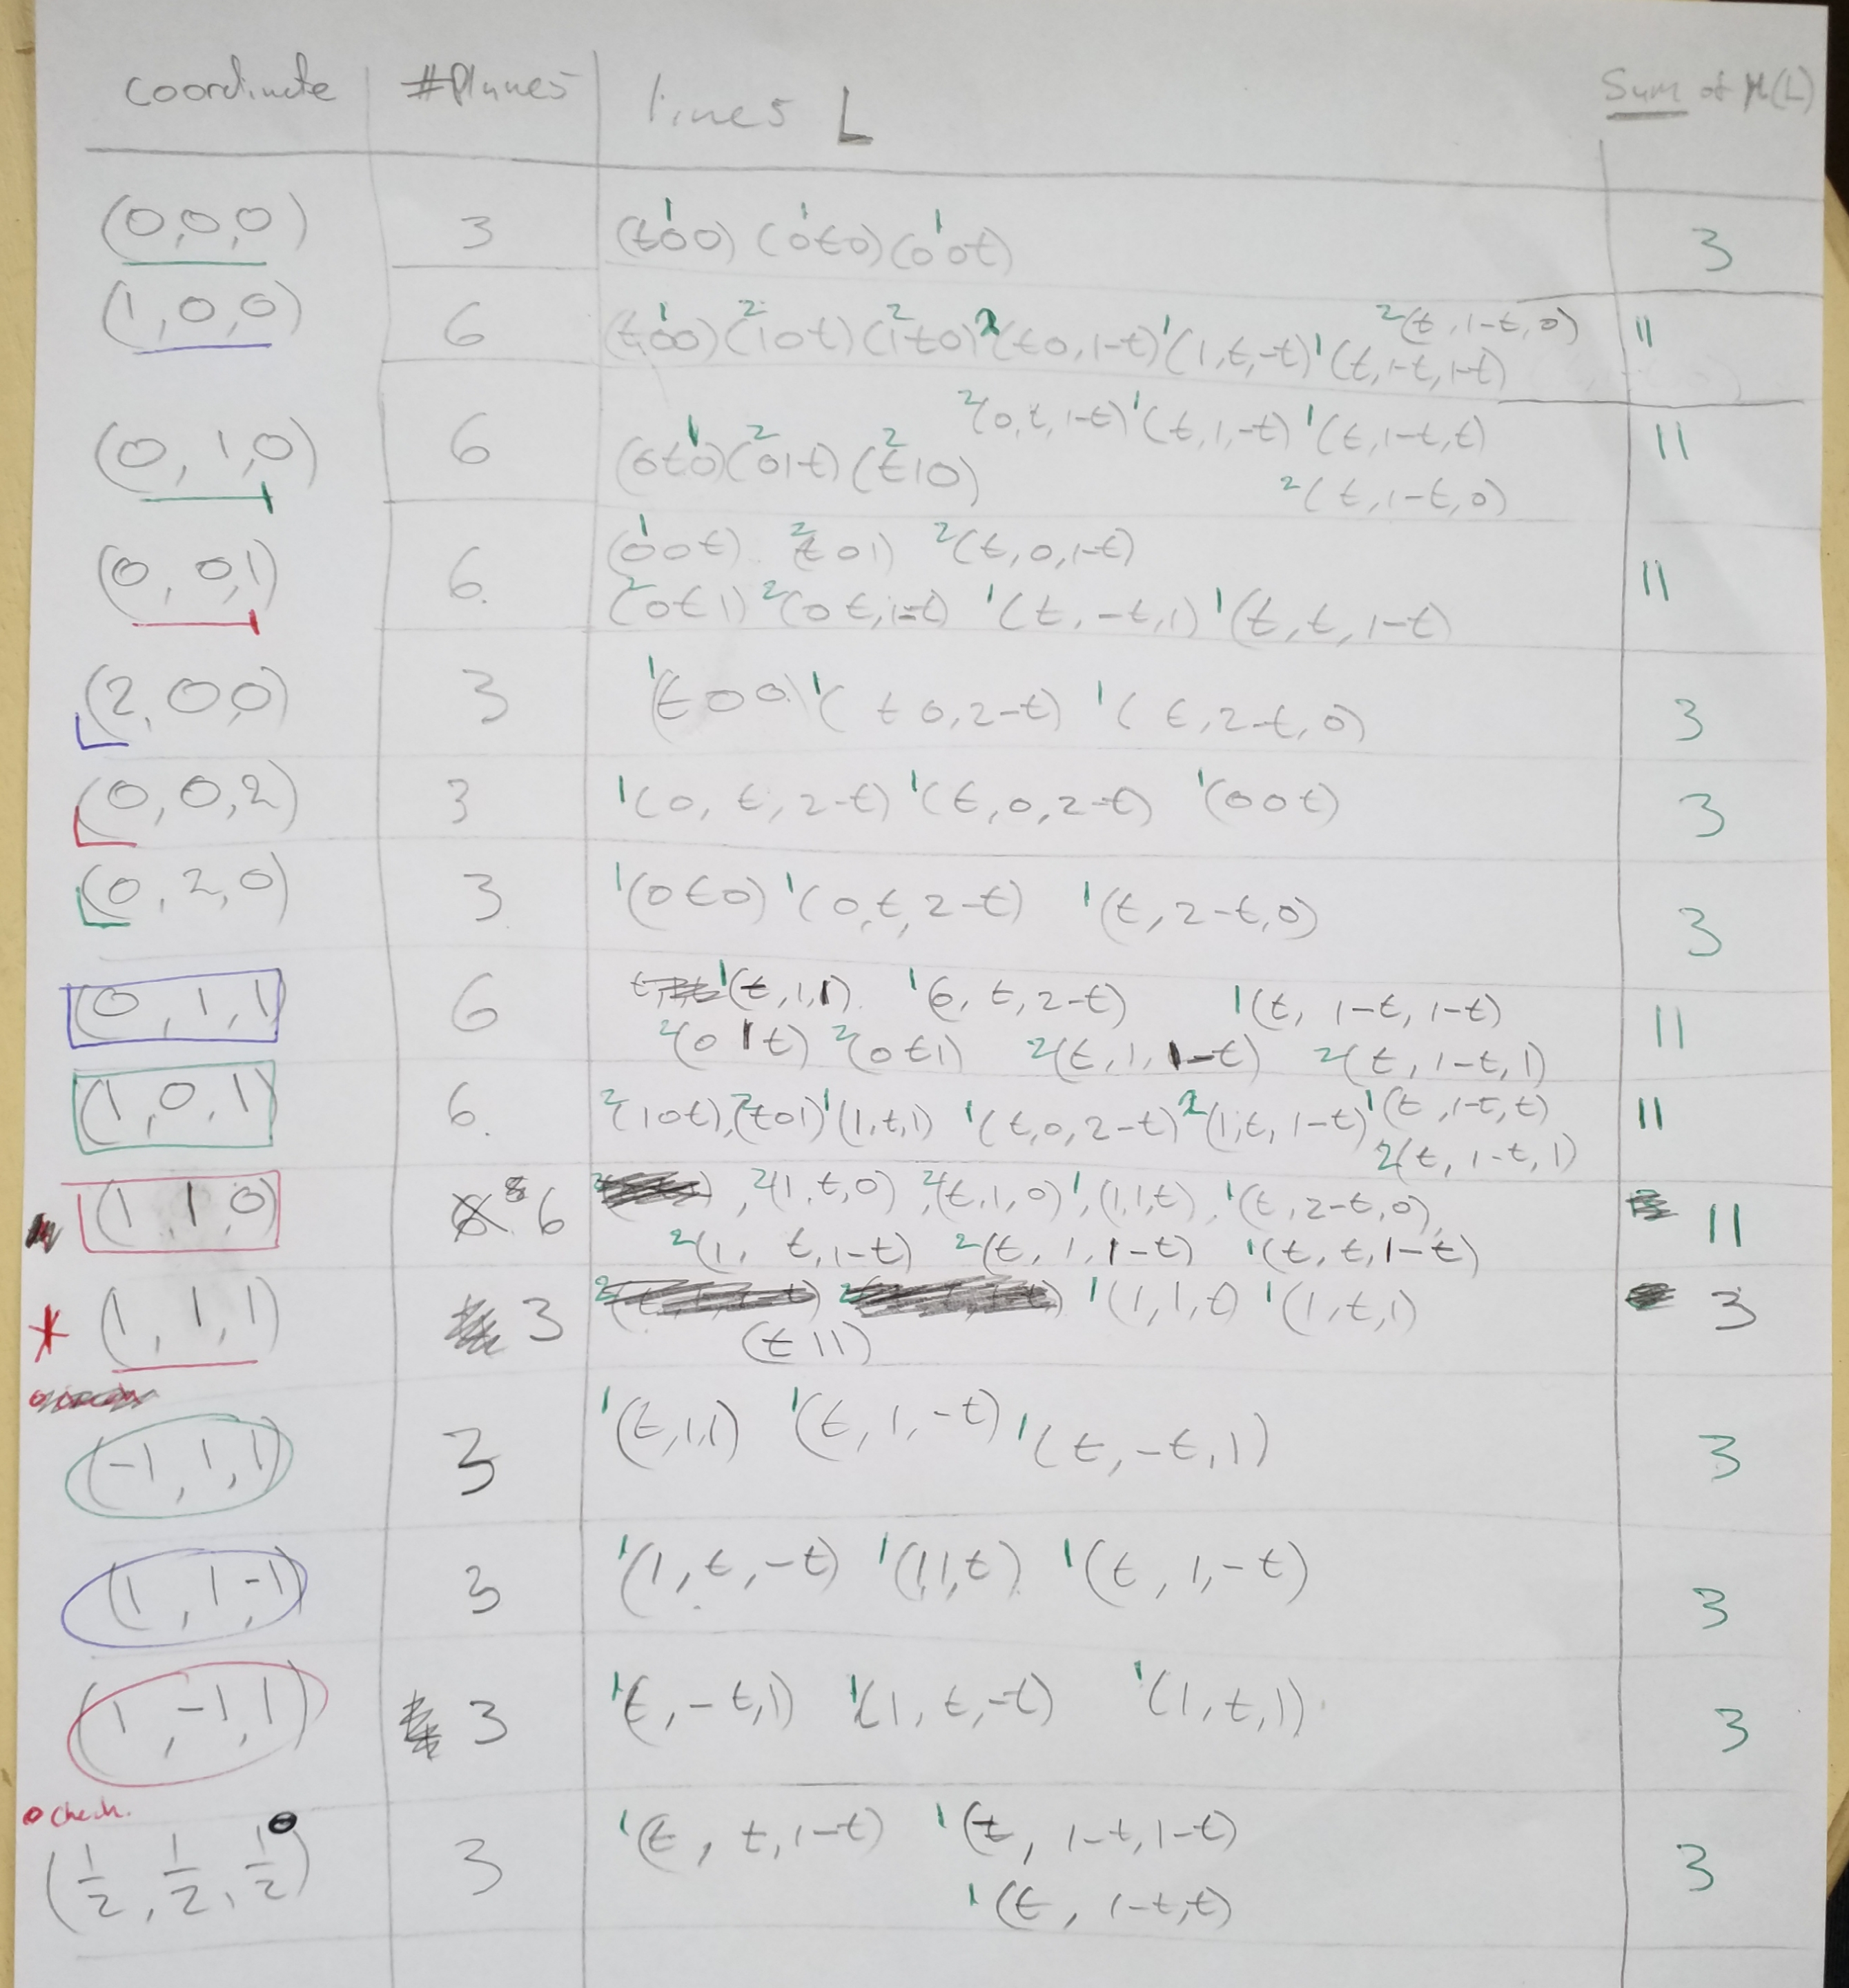
\includegraphics[scale=0.10,angle=0]{29072020 pics/mobpoints.jpg}  
    \caption{Determining the Möbius value of points in poset}
    \label{fig 4}
\end{figure}

For points determined by three planes the Möbius value is $-1$ as, 

$$\mu(\mathbb{R}^3) + \sum_{P\in \mathcal{A}} \mu(P) + \sum_{L \text{given lines}} L + \mu(pt) =0$$
which is,
$$1 -3 + 3 +\mu(pt)=0$$
and so $\mu(pt)=-1$. For points determined by six planes we similarly have,

$$1 -6 +11-\mu(pt)=0,$$

and so $\mu(pt)=-6$. Of the fifteen points we have nine points with $\mu(pt)=-1$ and six points with $\mu(pt)=-6$. Of the $27$ lines we have fifteen of $\mu(L)=1$ and twelve of $\mu(L)=2$. We also have eleven planes in $\mathbb{R}^3$. The characteristic polynomial is therefore,


\begin{align*}
\chi_{\mathcal{A}} (t) &=t^{3} -11t^{2} +(15+12*2)t - (9 * 1 +6*6)\\
&= t^{3} -11t^{2} +39t - 45.
\end{align*}


Applying theorem \ref{Zas} and letting $t=-1$, we have $r(\mathcal{A})=96$. Letting $t=1$, we have $b(\mathcal{A})= 16$. This agrees which the $b(\mathcal{A})$ value we expected. The following diagrams of $\mathcal{A}$ were make using Geoalgebra.

\begin{figure}[H]
    \centering
 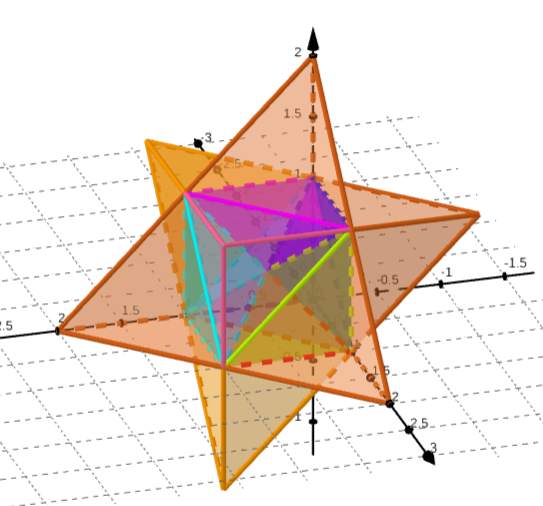
\includegraphics[width=.3\textwidth,angle=0]{29072020 pics/regions1.png}\qquad \qquad 
 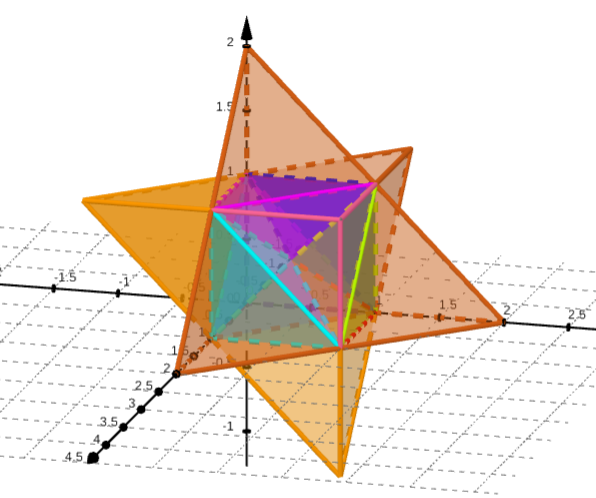
\includegraphics[width=.3\textwidth,angle=0]{29072020 pics/regions2.png}  
    \caption{Bounded regions of $\mathcal{A}$}
    \label{Bounded regions}
\end{figure}

In order to visualise the regions in the $\mathbb{R}^3$ case, we removed the orange tetrahedrons of Figure \ref{Bounded regions} and then dissected the cube according to the hyperplanes. 

\begin{figure}[H]

\centering
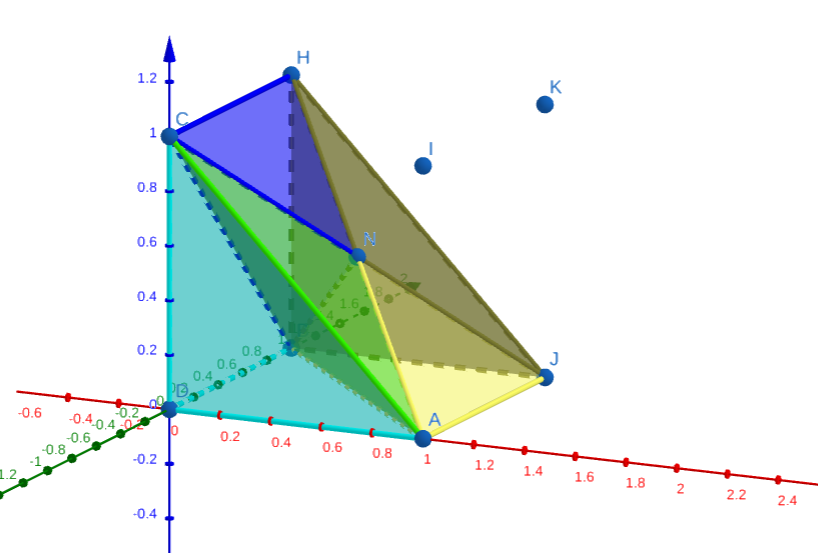
\includegraphics[width=.3\textwidth]{29072020 pics/1Figxz.png}\hfill
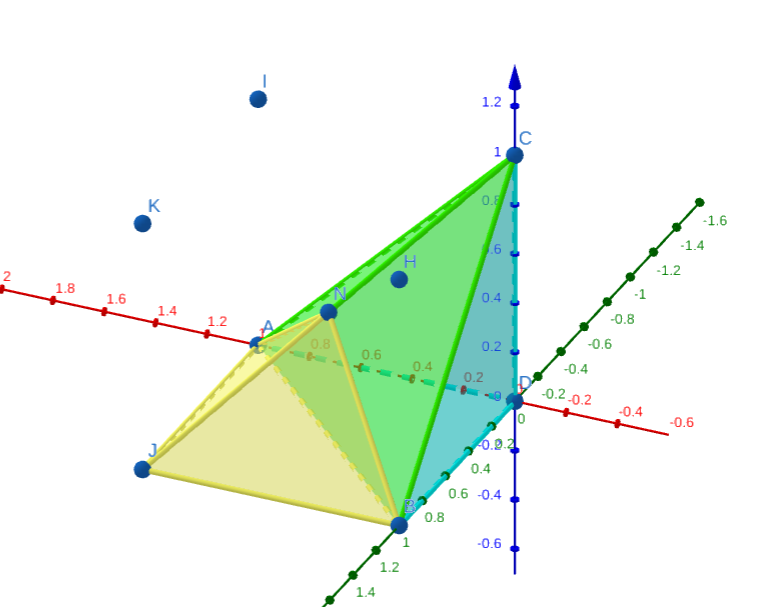
\includegraphics[width=.3\textwidth]{29072020 pics/2Figyz.png}\hfill
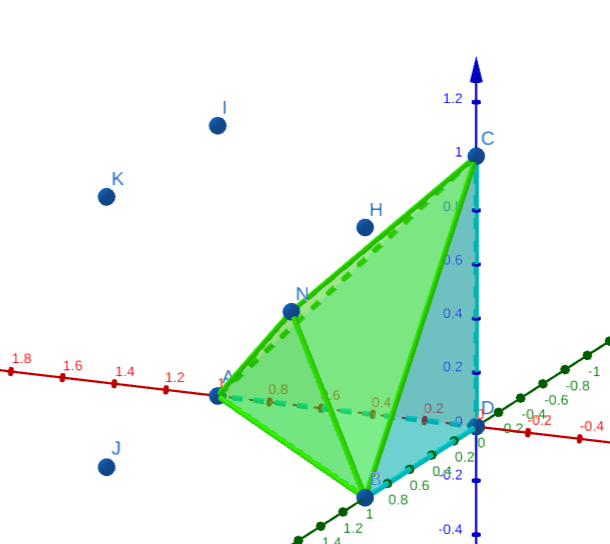
\includegraphics[width=.3\textwidth]{29072020 pics/3Figxy.png}

\caption{Cube cut by $x_{1,3}^1$, $x_{2,3}^1$ and $x_{1,2}^1$}
\label{cuts}
\end{figure}

On the right of Figure \ref{cuts} the blue and green region are one region until it is cut by $x_{123}^1$. This gives the ten regions in total with respect to symmetry. Lastly we show the corners of the arrangement given by $x_{123}^{1,2}$.

\begin{figure}[H]
\begin{center}
    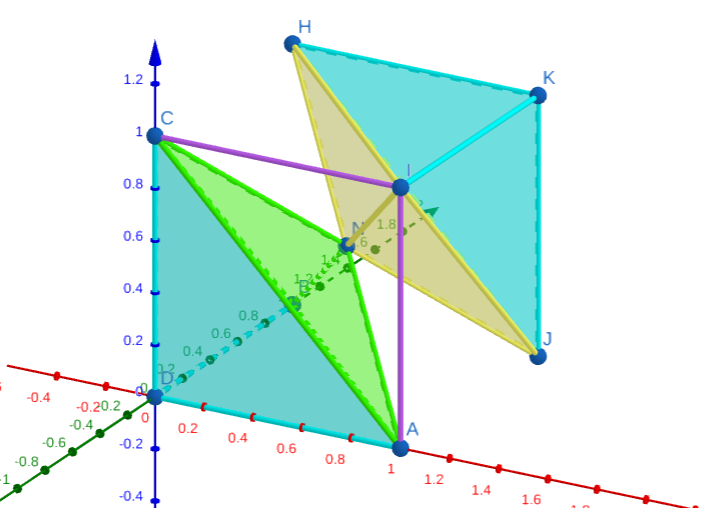
\includegraphics[width=.5\textwidth]{29072020 pics/2regionsINV.png}
\caption{Corners}
\label{}
\end{center}
\end{figure}
\end{example}

\section{Toric Case: Basic terminology and applications}

We will follow the theory described in \cite[p.9-15]{Ehrenborg2008AffineArrangements} and apply it to $H(S,k)$. By considering the quotient map $\mathbb{R}^n \rightarrow \mathbb{R}^{n} / \mathbb{Z}^n$, we consider only one representative for each class of hyperplanes i.e. hyperplanes of a family of a given type are identified to those that have: no change in variables and are translates, for example $x_{123}=1,2$, whereas $x_{12}=1$,$x_{13}=1$ and $x_{23}=1$ are distinct. In particular $x_i^{0} \sim x_i^{1} $ and for which we see each corner of the cube being identified with $\underline{0}$, and parallel edges also being identified. When we construct  $L(\mathcal{A})$ of $\mathbb{R}^3/\mathbb{Z}^3$, we only consider $x_{123}^{1}$ in comparison to $x_{123}^{1}$ and $x_{123}^{2}$ in $\mathbb{R}^3$. 


\begin{example} Here we show a toric arrangement with characteristic equation and distinguish how regions are identified and counted. Applying theorem \ref{readdy} gives the correct number of regions. 
\begin{figure}[H]
    \centering
 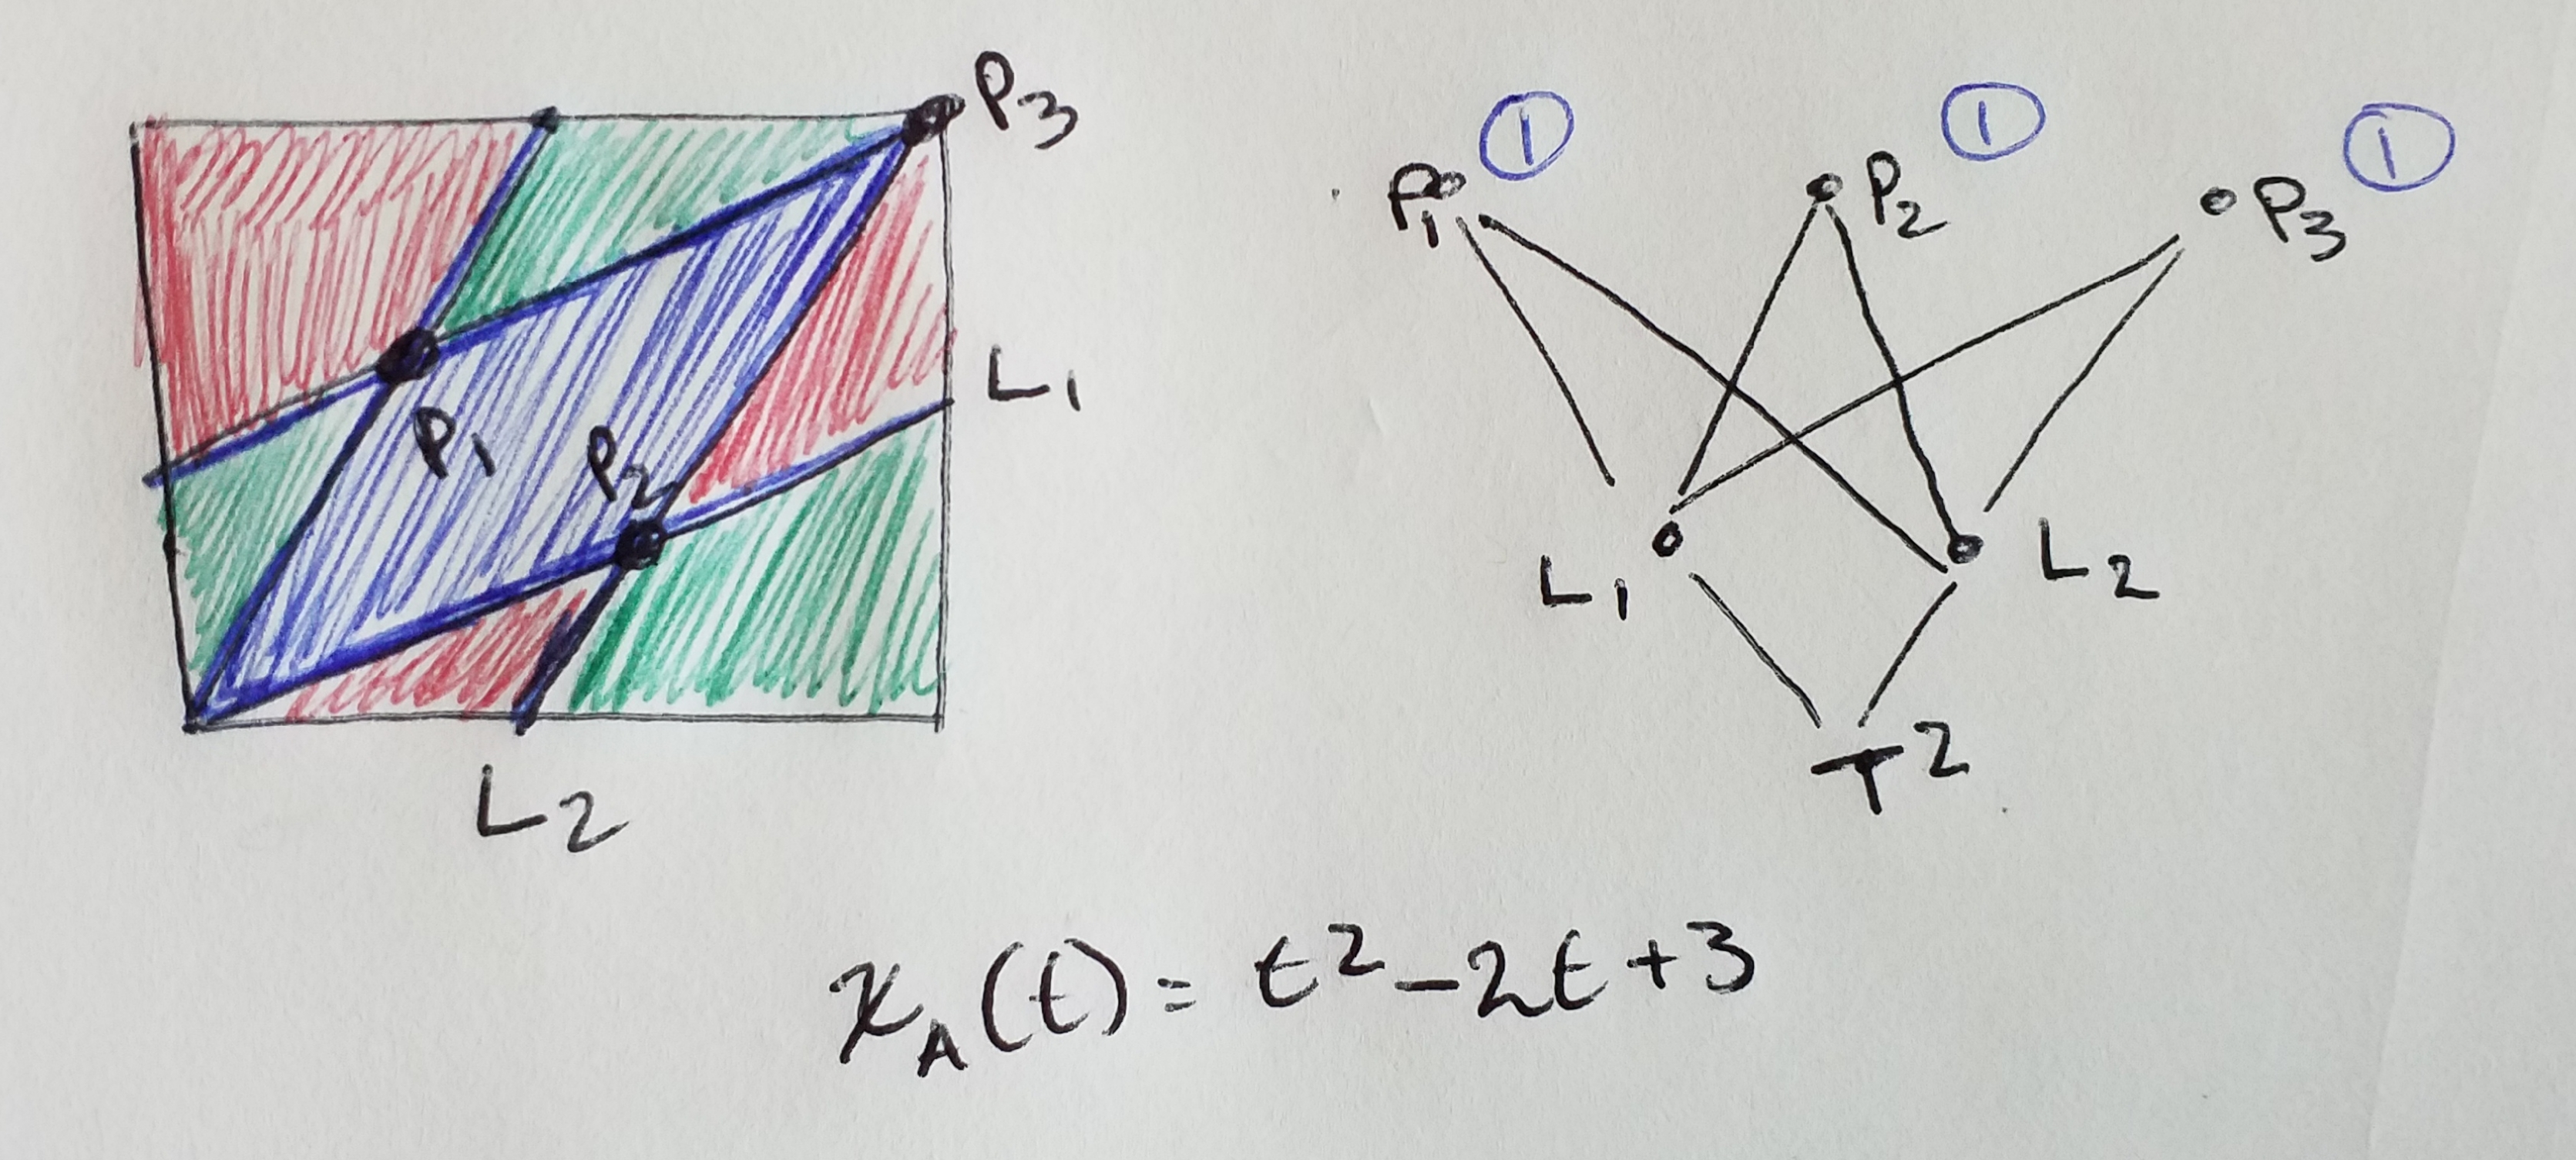
\includegraphics[scale=0.12,angle=0]{29072020 pics/toricposet.jpg}  
    \caption{}
    \label{}
\end{figure}
\end{example}

\begin{example} Consider the following toric arrangement, note the lines $H_4$ and $H_5$ giving the square $[0,1]^2$. 
\begin{figure}[H]
    \centering
 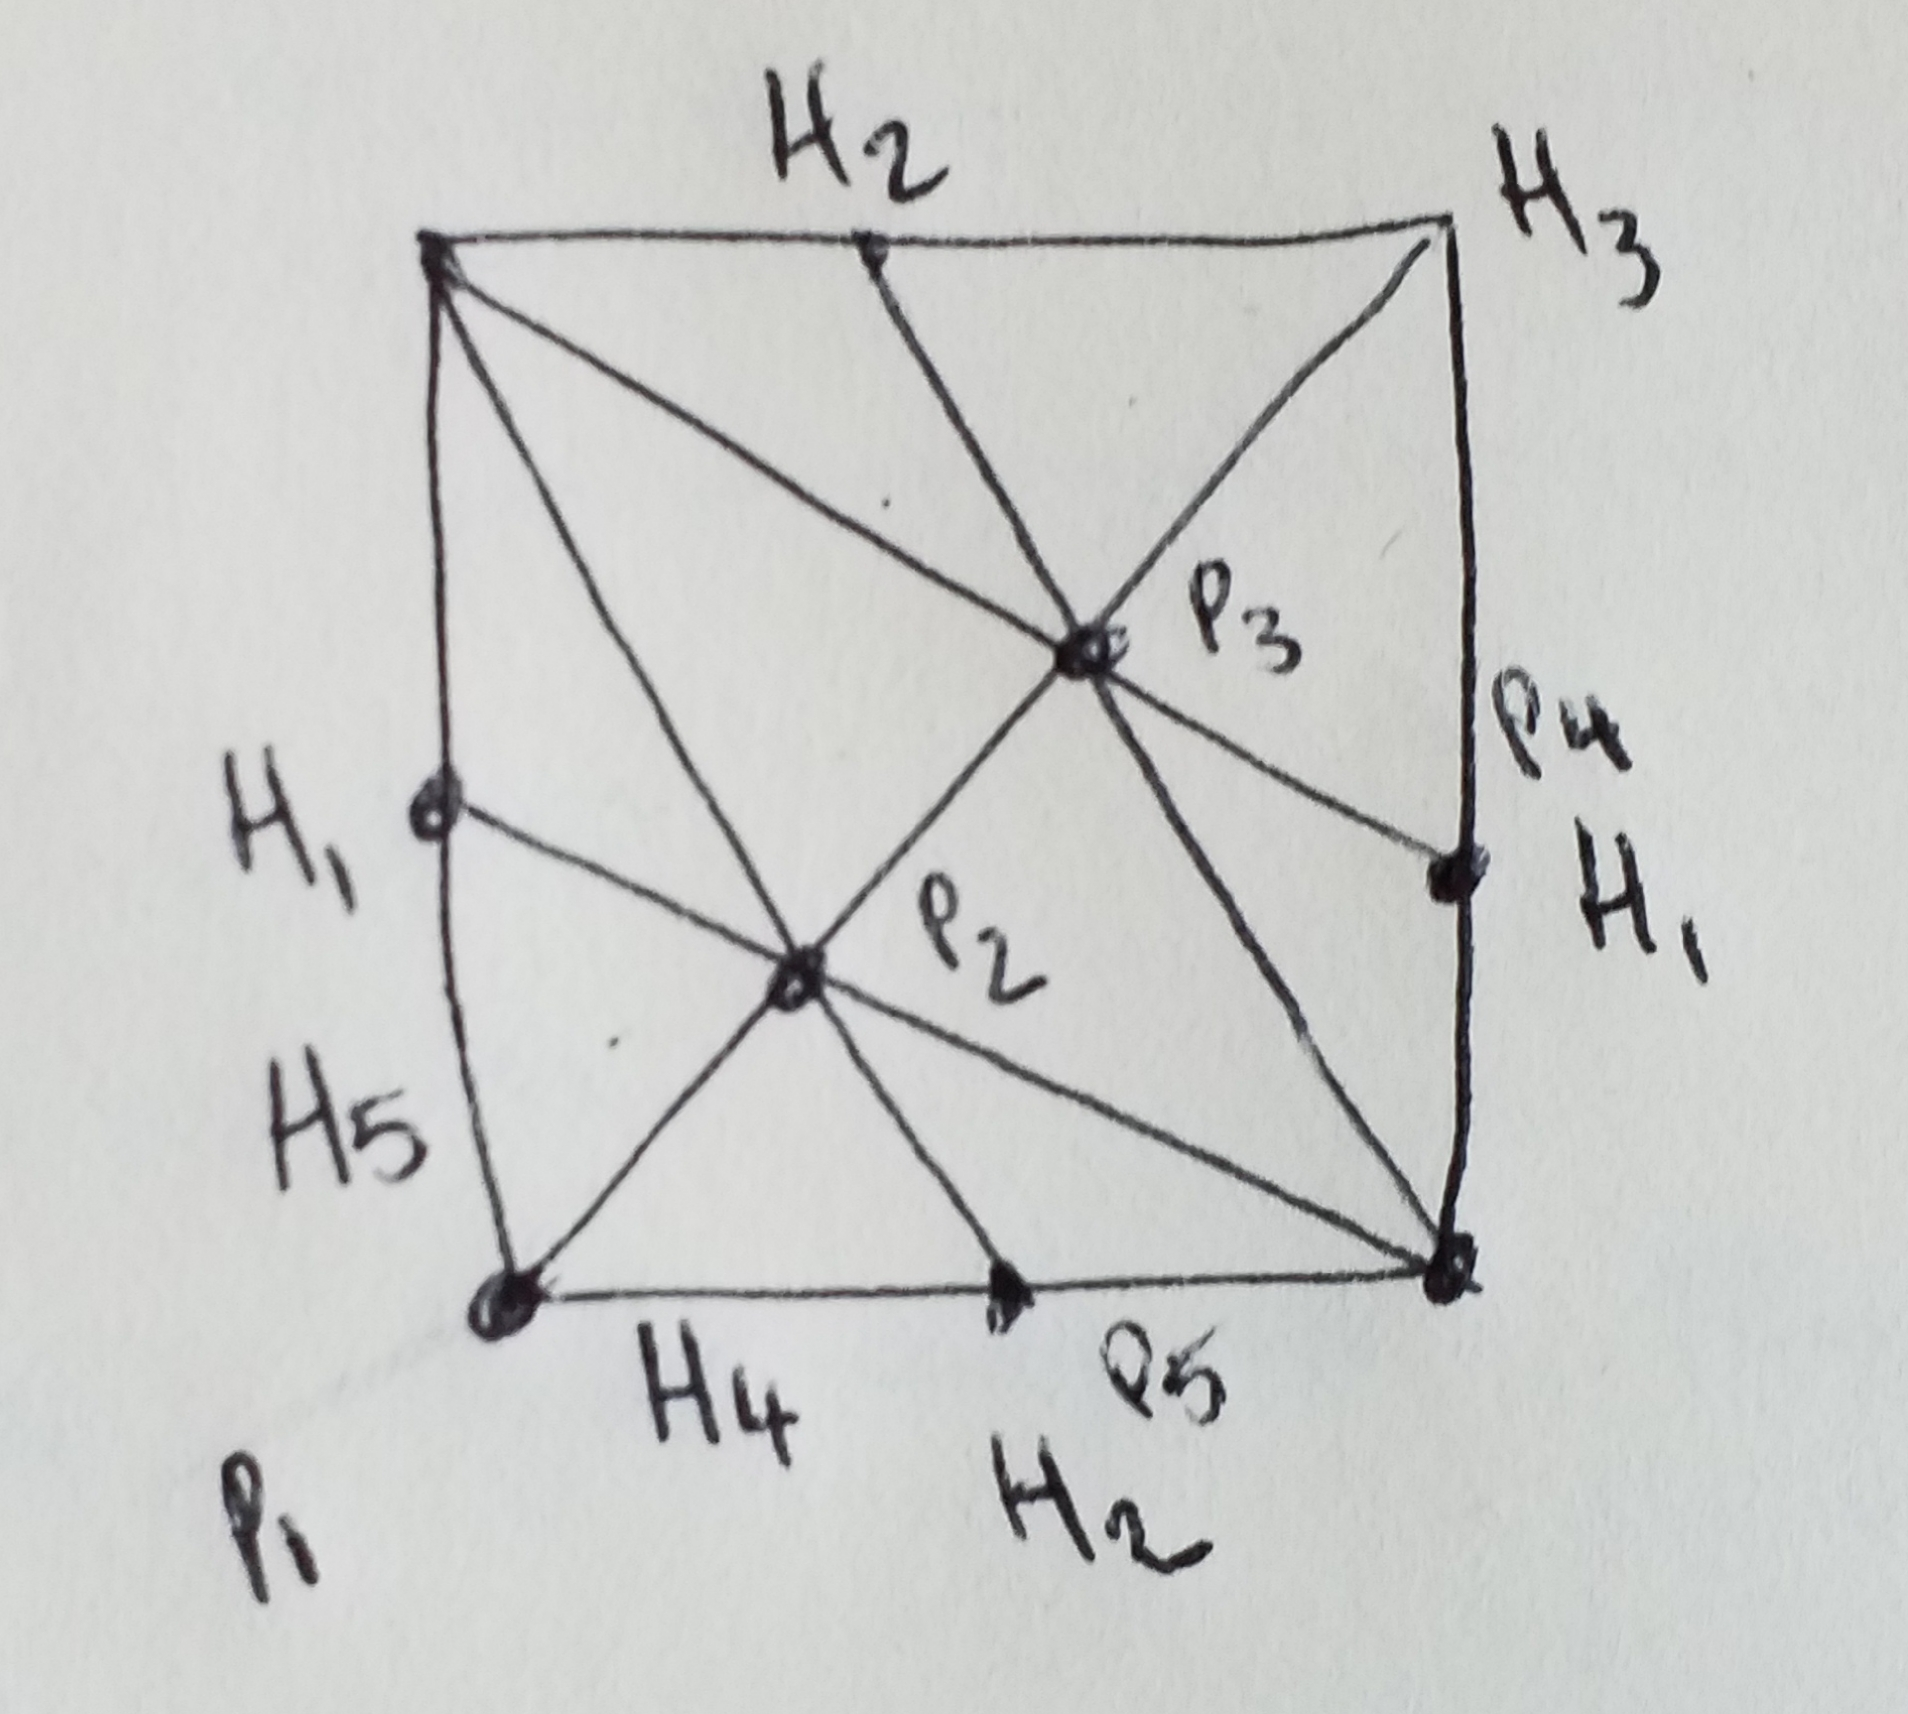
\includegraphics[width=.36\textwidth,angle=0]{29072020 pics/torichyperwalls.jpg}\qquad \qquad 
 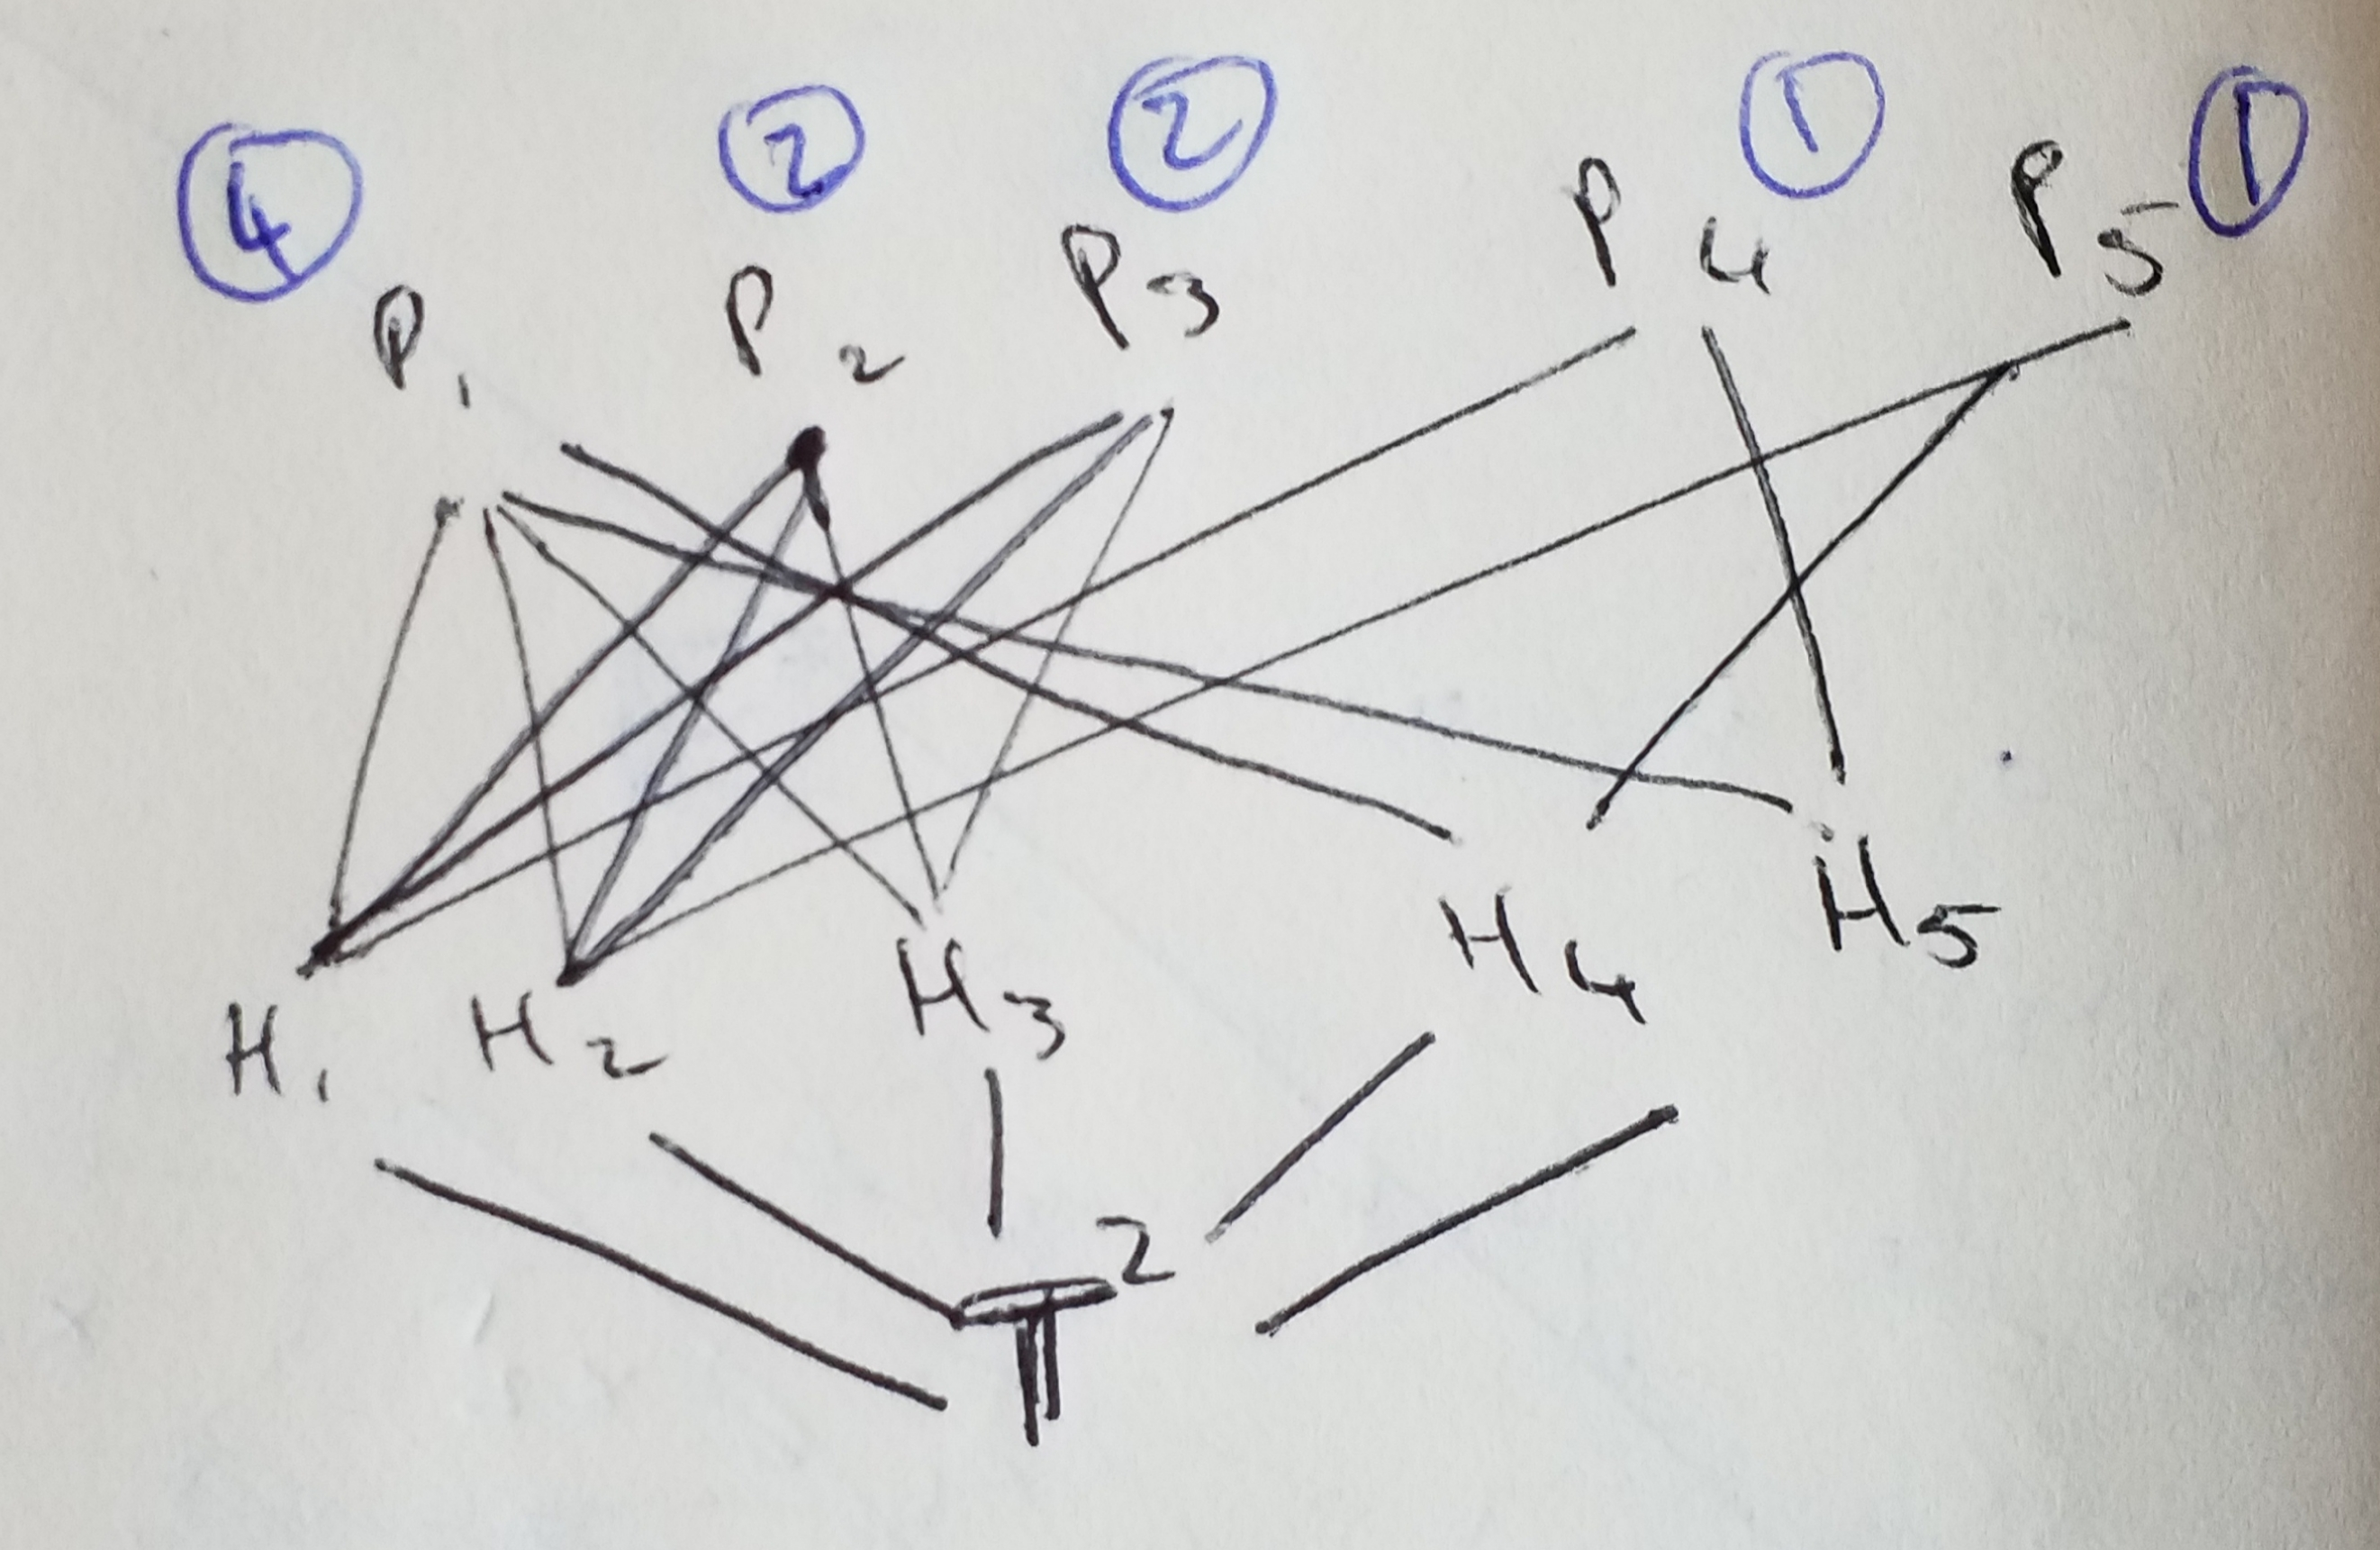
\includegraphics[width=.5\textwidth,angle=0]{29072020 pics/torichyperwall2.jpg}  
    \caption{Walls of hypercube}
    \label{}
\end{figure}

The characteristic of the following arrangement is $\chi_{\mathcal{A}} (t)=t^2 -5t+10$, hence we have $10$ regions.
\end{example}

We now give the toric analogue of theorem \ref{Zas}. The following result is by Ehrenberg-Readdy who used a valuative approach for torus arrangements and is derived from the Euler characteristic with the Euler characteristic for torus being $0$.


\begin{theorem}[\cite{Ehrenborg2008AffineArrangements}, Theorem 3.6]\label{readdy}
Let $\mathcal{A}$ be a toric hyperplane arrangement on the $n$-dimensional torus $T^n$
that subdivides the torus into regions that are open $n$-dimensional balls. Then the number of regions in the complement of the arrangement is given by 
$$(-1)^{n} \cdot \chi(\mathcal{A};t = 0)$$.
\end{theorem}


\subsection{Applying Zaslavsky's theorem to $H(S,k)$ in $\mathbb{R}^2/\mathbb{Z}^2$ and $\mathbb{R}^3/\mathbb{Z}^3$}

The aim of this section is to re-obtain the values $b(\mathbb{A})=2$ in $\mathbb{R}^2/\mathbb{Z}^2$ case and $b(\mathbb{A})=10$ in the $\mathbb{R}^3/\mathbb{Z}^3$ case.


\begin{example} The case $\mathbb{R}^2/\mathbb{Z}^2$ is similar to the affine case, with the notable exception of the corners of the square being identified.
\begin{figure}[H]
    \centering
 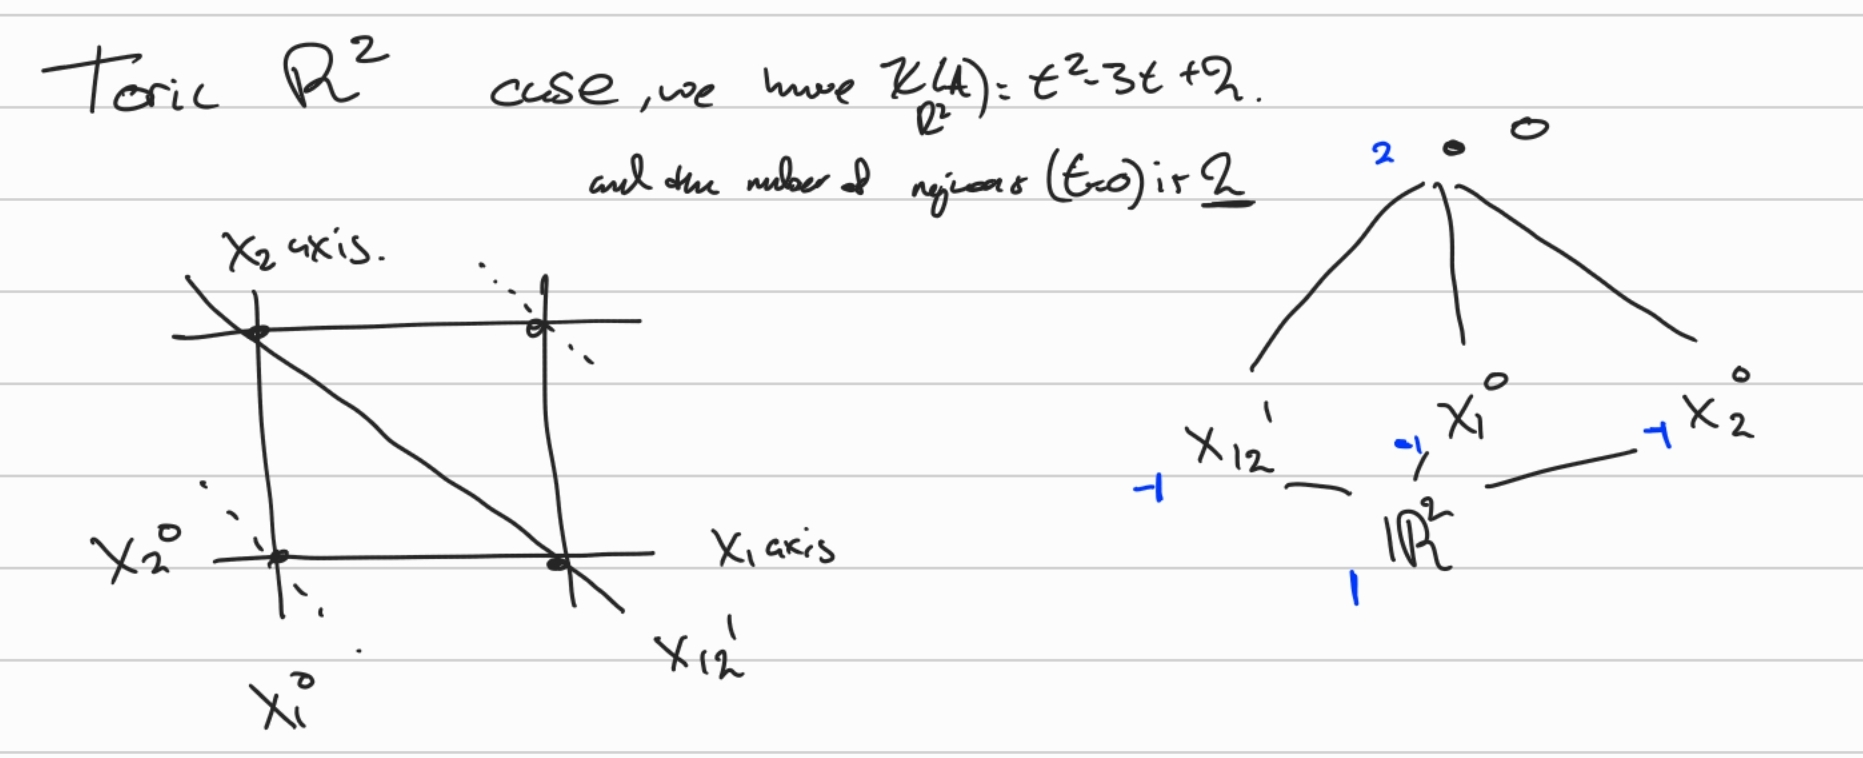
\includegraphics[scale=0.25,angle=0]{29072020 pics/ToricR2.jpg}  
    \caption{}
    \label{}
\end{figure}

\end{example}

\begin{example} We start by quotienting out $\mathbb{Z}^3$ from the $\mathbb{R}^3$ case. The flats in $L(\mathcal{A})$ are: the points $\underline{0}, \underline{\frac{1}{2}}$, the black, blue (ignore black lines) and purple lines (ignore black lines) respectively in Figure \ref{toricfig1}, and the hyperplanes ($x_i^{0},x_{ijk}^{1},x_{ij}^1$). Note black axis lines, blue lines and purple lines meet $\underline{0}$. The purple lines also meet the point $\underline{\frac{1}{2}}$.

\begin{figure}[H]
    \centering
 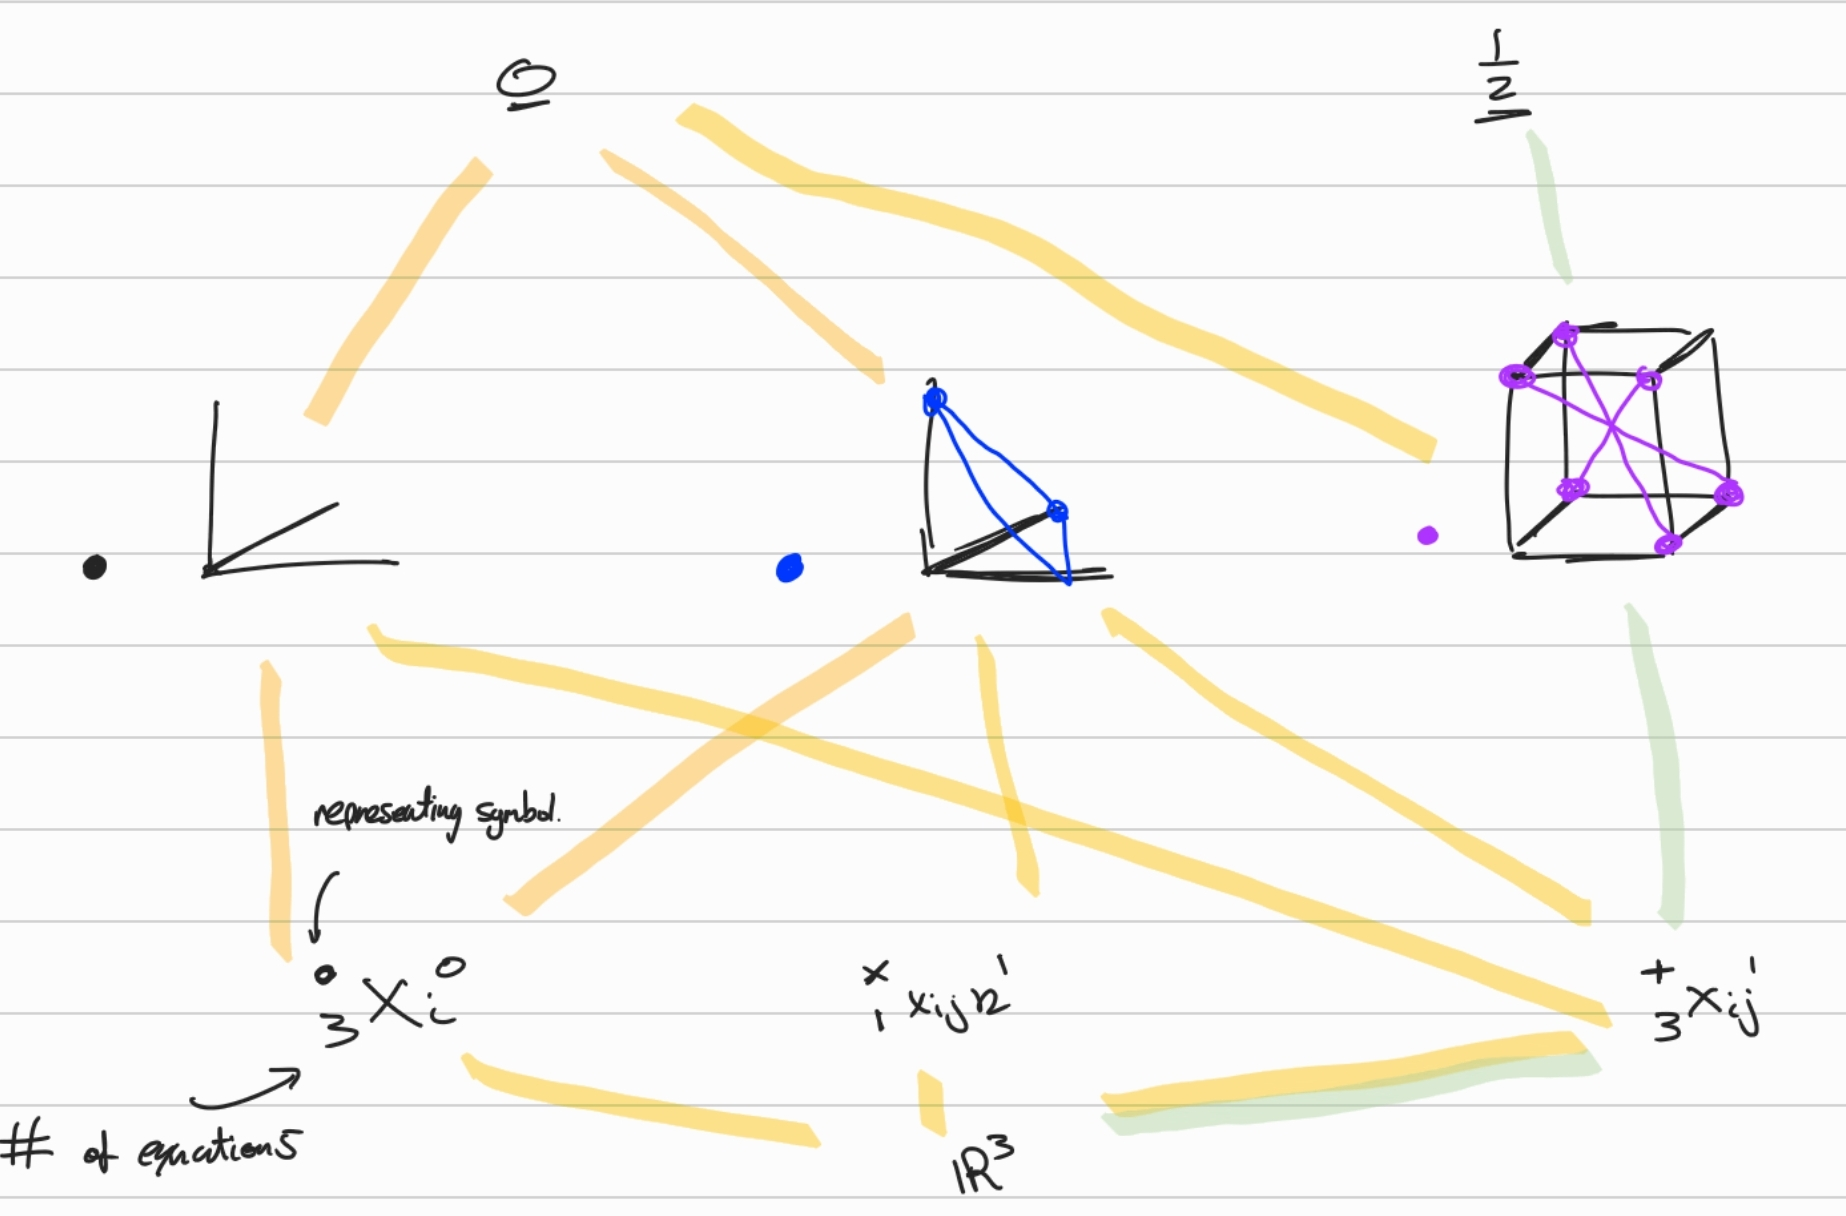
\includegraphics[scale=0.25,angle=0]{29072020 pics/1ToricR3.jpg}  
    \caption{}
    \label{toricfig1}
\end{figure}

To reduce complexity Figure \ref{toricfig2} shows $L(\mathcal{A})$, drawn in parts (only drawing the inclusion of each object into the level below). 

\begin{figure}[H]
    \centering
 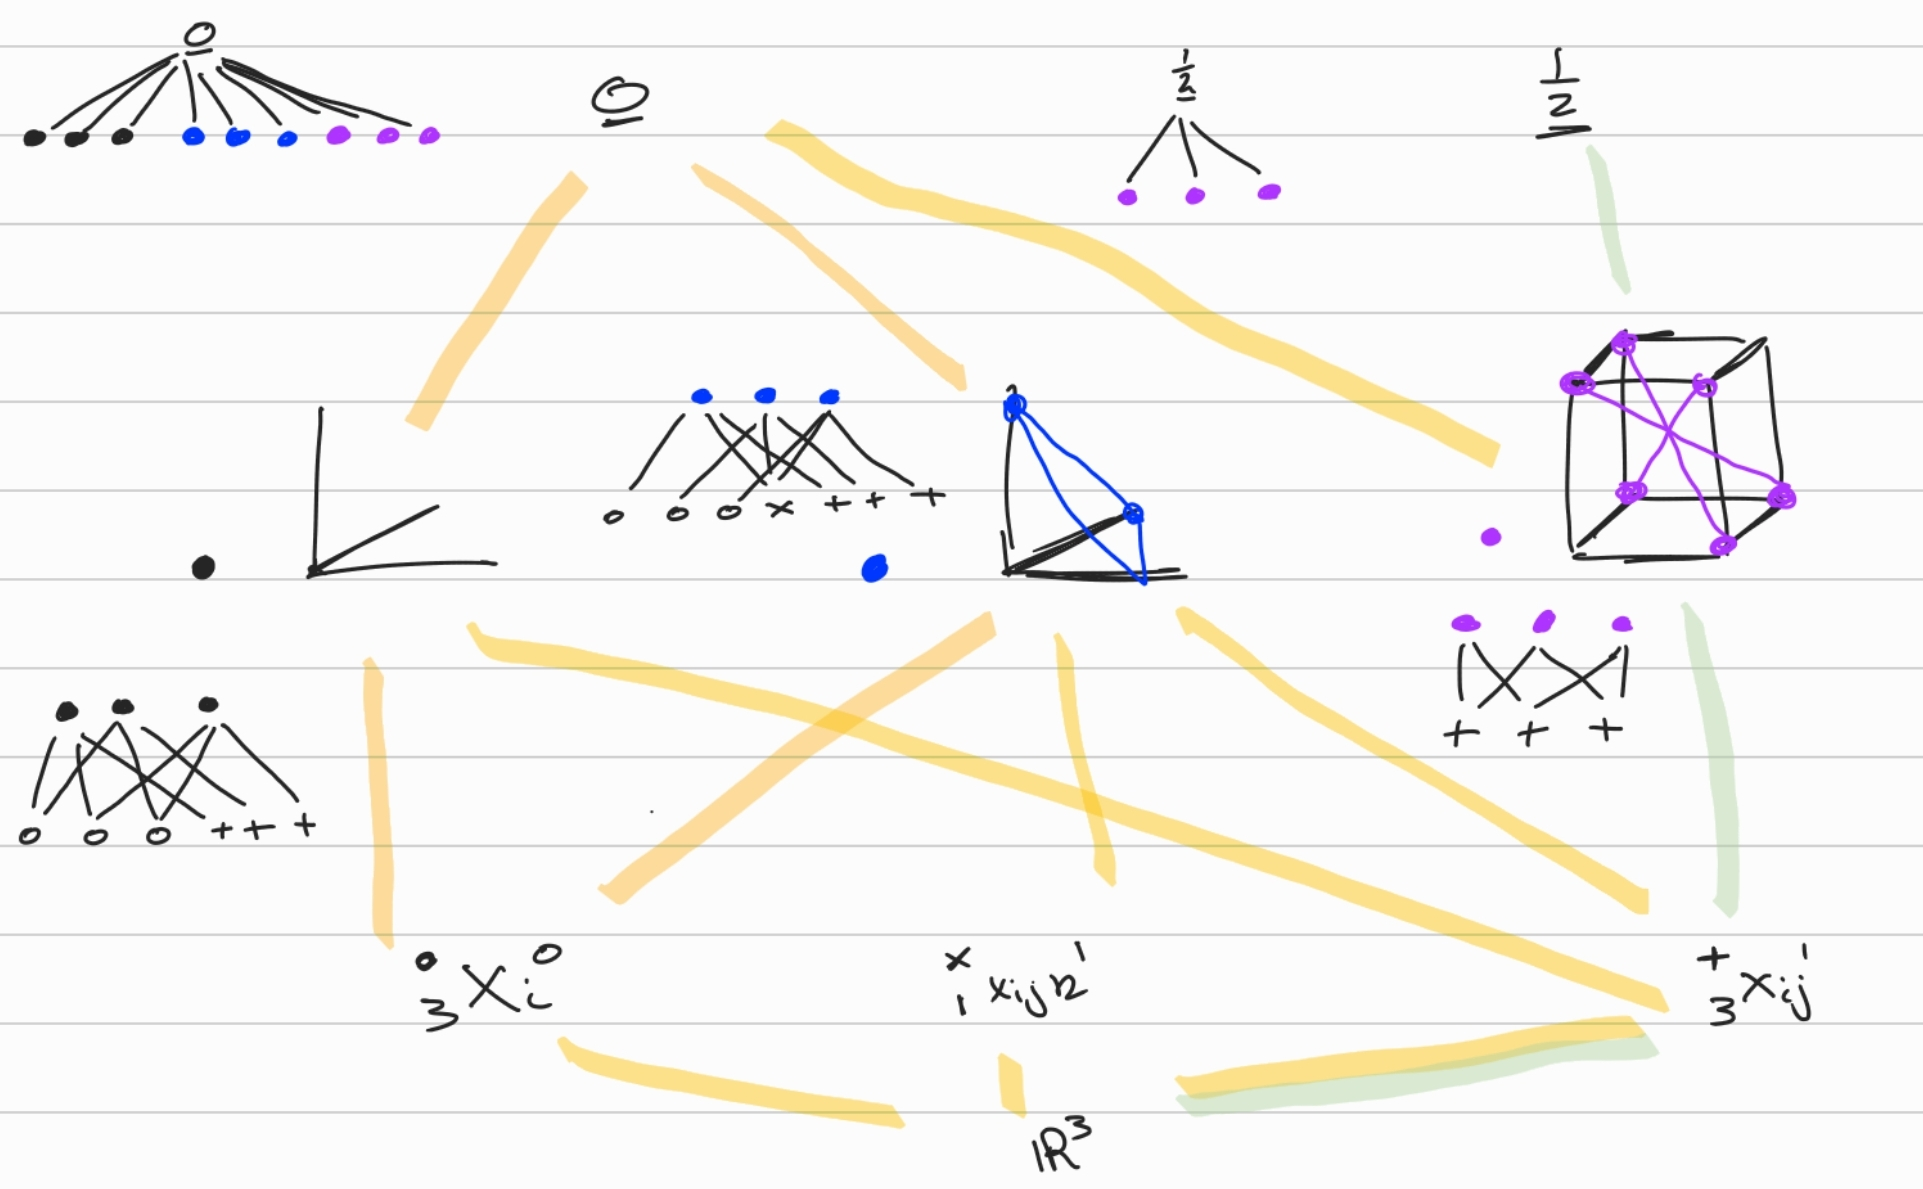
\includegraphics[scale=0.25,angle=0]{29072020 pics/2ToricR3.jpg}  
    \caption{}
    \label{toricfig2}
\end{figure}

Next we determine the mobius values for the lines. 

\begin{figure}[H]
    \centering
 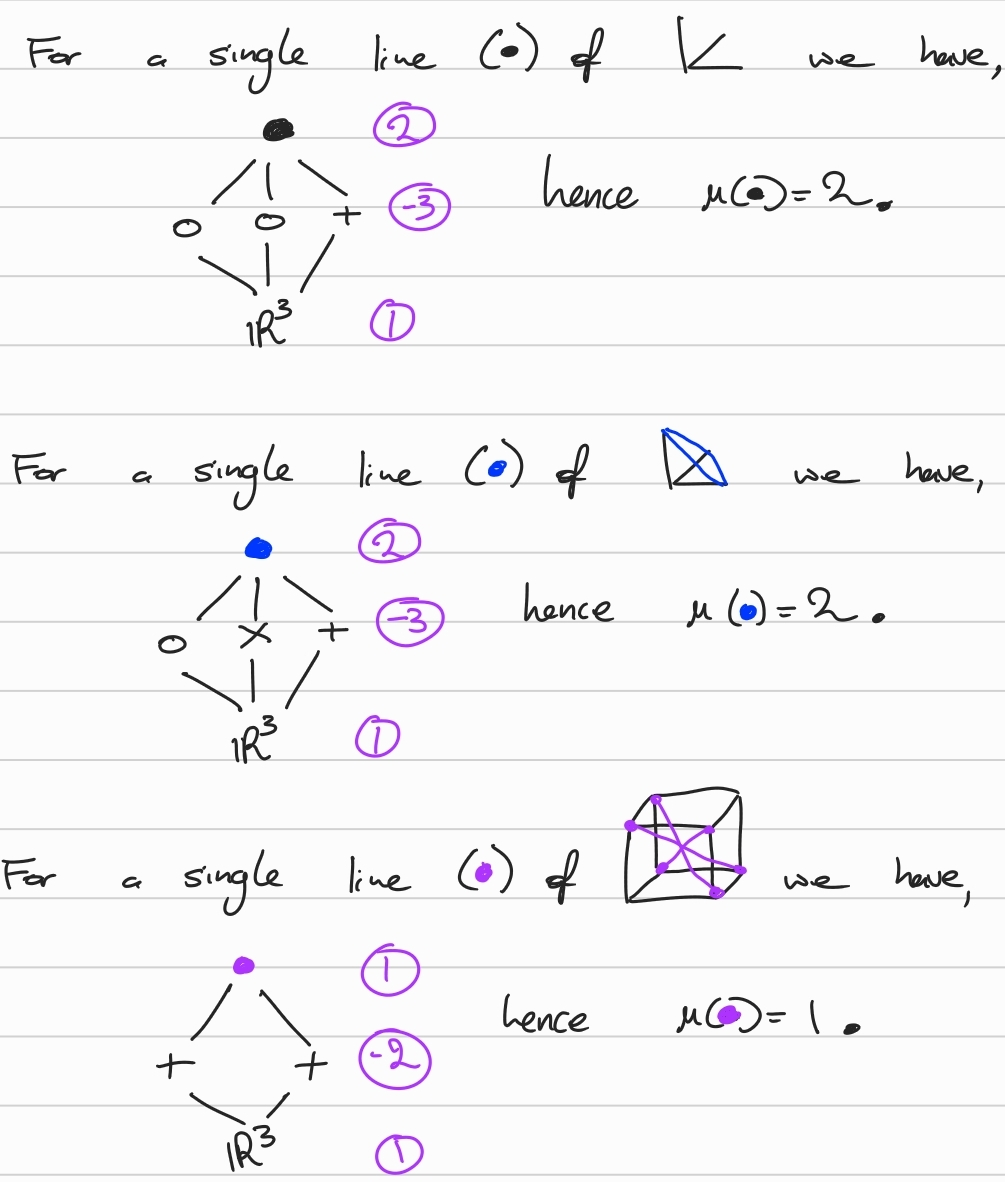
\includegraphics[scale=0.25,angle=0]{29072020 pics/3ToricR3.jpg}  
    \caption{}
    \label{}
\end{figure}

 Next we determine the Mobius values of the points $\underline{0}, \underline{\frac{1}{2}}$. To reduce complexity group the lines and planes and attach a multiple for the number of times they appeared, then respectively multiplying the Mobius value by this value.

\begin{figure}[H]
    \centering
 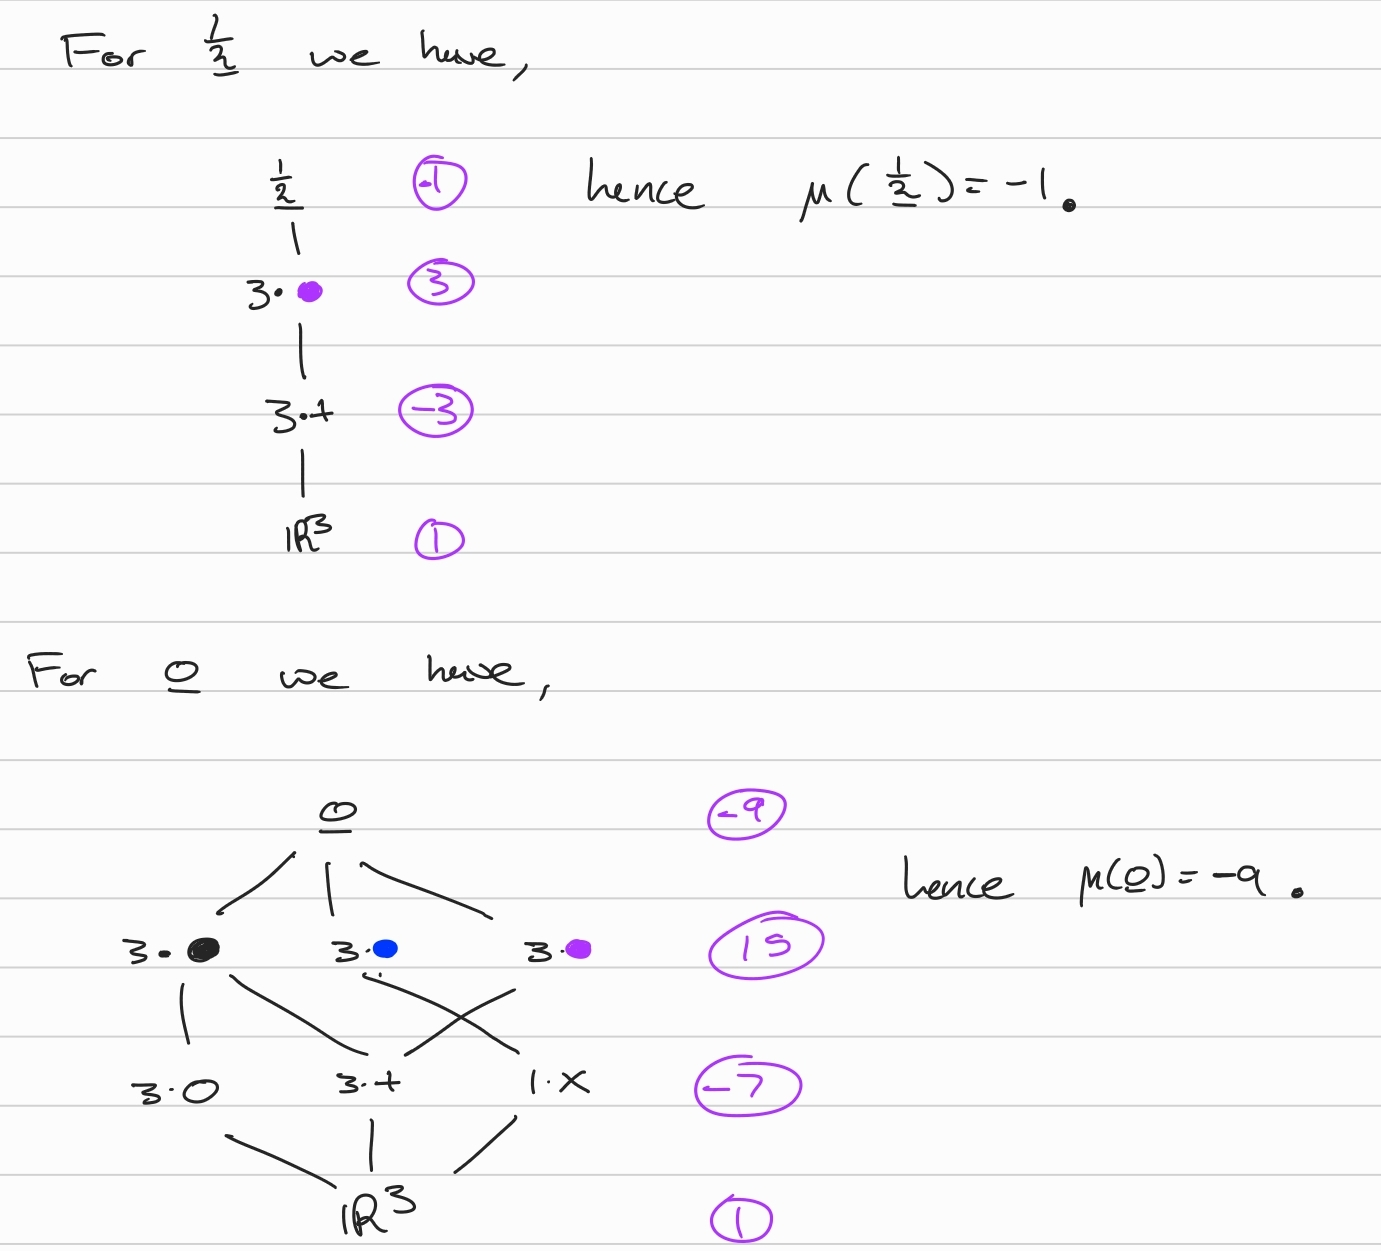
\includegraphics[scale=0.25,angle=0]{29072020 pics/4ToricR3.jpg}  
    \caption{}
    \label{}
\end{figure}

As we have determined the mobius values for the points, by Theorem \ref{readdy} we have $10$ regions. 

\end{example}

\printindex

\bibliographystyle{alpha}
\bibliography{bibtex}



\end{document}


